%% Bookheader, Nov 8, 2020; July 18, 2022

\documentclass[11pt]{../Support/ourbook}
%% or for landscape, comment out line above and use this one:
%%\documentclass[landscape,11pt]{ourbook}

%% This will keep space from stretching around display math:

\makeatletter
\renewcommand\normalsize{%
   \@setfontsize\normalsize\@xipt{13.6}%
   \abovedisplayskip 11\p@  \@minus6\p@
   \abovedisplayshortskip \z@ 
   \belowdisplayshortskip 6.5\p@ \@minus3\p@
   \belowdisplayskip \abovedisplayskip
   \let\@listi\@listI}
\makeatother
\normalsize


\begin{document}
\tableofcontents
\graphicspath{{../../Chapters/matter_energy_intro/en_US}}
\chapter{Introduction to the Kontinua Sequence}

This book will start you on the long and difficult trek to becoming a modern
problem solver. Along the path, you will learn how to use the tools of
math, computers, and science. 

Why should you bother? There are big problems in this world that will
require expert problem solvers. Those people will make the world a
better place while enjoying interesting and lucrative careers. We are
talking about engineers, scientists, doctors, computer programmers,
architects, actuaries, and mathematicians. Right now, those occupations represent
about 6\% of all the jobs in the United States. Soon,
that number is expected to rise above 10\%.  On average, people in
that 10\% of the population are expected to have salaries twice that
of their non-technical counterparts.\index{career}

Solving problems is difficult. At some point on this journey, you will
see people who are better at solving problems than you are. You, like
every other person who has gone on this journey, will think ``I have
worked so hard on this, but that person is better at it than
I am. I should quit.'' Don't.\index{quitting}

First, solving problems is like a muscle. The more you do, the better
you get at it.  It is OK to say ``I am not good at this yet.'' That
just means you need more practice.

Second, you don't need to be the best in the world. 10 million people
your age can be better at solving problems than you, \textit{and you
  can still be in the top 10\% of the world}. If you complete this
journey, there will be problems for you to solve and a job where your
problem-solving skills will be appreciated.

So where do we start?

\section{Matter and Energy Introduction}

The famous physicist Richard Feynman once asked this question: ``If,
in some cataclysm, all of scientific knowledge were to be destroyed,
and only one sentence was passed on to the next generation of
creatures, what statement would contain the most information in the
fewest words?''

His answer was ``All things are made of atoms—little particles that move around in
perpetual motion, attracting each other when they are a little
distance apart, but repelling upon being squeezed into one another.''

That seems like a good place to start.\index{atom}

All things (including the air around you) are made of atoms. Atoms are
very tiny -- there are more atoms in a drop of water than there are
drops of water in all the oceans.
% ADD: If you want a better visual of the scale: https://htwins.net/scale2/, start at around 10^-8

Every atom has a nucleus that contains protons and neutrons. There is also
a cloud of electrons flying around the nucleus. However, the mass of the atom
comes mainly from the protons and neutrons, which are exponentially heavier
than electrons.\index{protons} \index{neutrons} \index{electrons}

\includegraphics[width=1\textwidth]{atom1.png}

Watch \textbf{Elements and atoms} from Khan Academy at \url{https://youtu.be/IFKnq9QM6_A}.

\subsection{Models of the Atom} 
Over the history of science, there have been many ideas about the structure of 
atoms. This history is a good example of how science develops: how unexpected 
results drive scientists to update their models, moving us closer and closer to 
a true model of the atom. During his investigations into the behavior of gases, 
John Dalton (lived 1766-1844) noted that different elements combine in strict 
ratios. For example, he noted that nitrogen and oxygen combine in a 1:1 and 1:2 
fashion, but no ratio in between.

This first model of the atom is very rudimentary: each element is a unique atom, 
and atoms cannot be subdivided. The atom is modeled as one large, solid, uniform, 
and neutral object. Some scientists, including the British physicist J.J. Thomson 
(1856-1940) thought that larger atoms (like lead) might be able to be broken down
into smaller atoms (like hydrogen). Thomson had been experimenting with cathode 
ray tubes and discovered that the these rays traveled much faster than thought 
possible for a particle the size of a hydrogen atom. This, combined with the 
observation that cathode rays could be deflected by electrical charge, led him to 
postulate two things:

\begin{enumerate}
\item atoms can be broken into parts much smaller than a hydrogen atom
\item whatever part of atoms that composes cathode rays is negatively charged
\end{enumerate}

The presence of "corpuscules" (as Thomson called them) that were negatively 
charged and smaller than a hydrogen atom contradicted Dalton's theory. Thomson 
updated his model of the atom: adding small, negatively charged subatomic 
particles (now called electrons) that were embedded in a larger, uniform, positive 
sphere. Suddenly, the atom went from neutral and indivisible to made of different 
types of charged particles. 

At the time, physicists were very interested in the mass-to-charge ratios of 
various particles (Thomson was able to determine the mass-to-charge ratio of the 
electron during his experiments), and Ernest Rutherford (1871-1937) was 
investigating the mass-to-charge ratio of alpha particles. (Alpha particles, we 
now know, are composed of two protons and two neutrons. They are emitted from 
certain radioactive elements, including uranium.) Rutherford needed consistent 
scattering of alpha particles in order to collect the data necessary to determine 
the particles' mass-to-charge ratio. He achieved this by bombarding extremely 
thin gold foil with alpha particles. The Thomson model of the atom would predict 
that particles would be slightly deflected, as illustrated below: 
FIXME insert thomson model scattering


However, a small but significant portion of the alpha particles were deflected 
over $90 \deg$! To explain this, Rutherford modeled the atom as mostly empty 
space with a small, dense, positive center (we now call this the nucleus).
FIXME rutherford model of the atom

At the same time that Rutherford was conducting his gold foil experiments, Niels 
Bohr was investigating the hydrogen line series FIXME insert figure of hydrogen 
lines. When hydrogen is electrically excited, it emits specific bands of color, 
not a complete spectrum. Bohr, upon learning of Rutherford's experiments, 
embraced the Rutherford model over the Thomson model and postulated that electrons 
existed only at discrete distances from the nucleus. When electrified, a hydrogen 
atom's electrons would gain energy and "jump" up one or more levels. The electron 
would be unstable in this energized state, and eventually "fall" back to the 
lowest energy level, emitting the extra energy as light. different colors of 
light have different energies: violet being the most energetic and red being the 
least. The different levels had differing amounts of energy between them, 
resulting in only those colors corresponding to the exact energy step between 
levels being emitted. This model, called the Bohr model or the Rutherford-Bohr 
model, expands on the Rutherford model by limiting electrons to specific 
distances from the nucleus, and is often compared to a model of the solar system 
FIXME add image of Bohr model. 

This is likely the model you are most familiar with seeing, and it is the one we 
will use often in this text. 


The previous graphic is slightly untrue. While it is a convenient model for 
thinking about atoms, in reality electrons don't neatly orbit the nucleus. 
Scientists don't know exactly where an electron will be in relation to the 
nucleus, but they do know where it's most likely to be. They use a cloud that is 
thicker in the center but fades out at the edges to represent an electron's 
position.


\includegraphics[width=.5\textwidth]{atomCloud.png}


We classify atoms by the numbers of protons they have. An atom with one proton is a
hydrogen atom, an atom with two protons is a helium atom, and so forth (refer to periodic table on pg..). We say that hydrogen and helium are \textit{elements} because the classification of elements is based on proton number. And we give
each element an atomic symbol. Hydrogen gets $H$. Helium gets $He$ Oxygen gets
$O$. Carbon gets $C$\index{elements}, etc.

Often two hydrogen atoms will attach to an oxygen atom. The result is
a water molecule. Why do they cluster together? because they share 
electrons in their clouds.\index{molecules}
% ADD:Electronegativity

A molecule is described by the elements it contains. Water is $H_2O$
because it has two hydrogen atoms and one oxygen atom.

There are many kinds of molecules. You know a few:
\begin{itemize}
\item Table salt is crystals made of $NaCl$ molecules: a sodium atom attached to a chlorine atom.
\item Baking soda, or sodium bicarbonate, is $NaHCO_3$.
\item Vinegar is a solution including acetic acid ($CH_3COOH$).
\item $O_2$ is the oxygen molecules that you breathe out of the air (Air, a blend of gases, is mostly $N_2$.).
\end{itemize}

\subsection{Reading the Periodic Table}
The Periodic Table organizes what we know about the structure of different 
elements. Each element has its own block or tile on the Periodic Table, and the 
information on the tile tells us about the structure of that atom. Take a look at 
the tile for carbon: (FIXME add carbon tile)

There are two key numbers: the atomic number and the average atomic mass. The 
atomic number tells how many protons there are in the nucleus of any atom of 
carbon. All carbon atoms have 6 protons. The other number is the average atomic 
mass. Have you heard of carbon-14 dating? The phrase "carbon-14" refers to a rare 
type of carbon that decays radioactively. By seeing how much carbon-14 has 
decayed, scientists can estimate the age of organic materials, such as bone or 
ash. Carbon-14 is a radioactive isotope (or version) of carbon. The 14 refers to 
the mass number - the total amount of protons AND neutrons in the nucleus. The 
most common isotope of carbon is carbon-12, with 6 protons and 6 neutrons in its 
nucleus. Carbon-14, on the other hand, has 8 neutrons, which makes the nucleus 
unstable, leading to radioactive decay. FIXME tow models comparing the structure 
of  C-12 and C-14. FIXME resource: atom builder PhET. The average atomic mass is 
the weighted average of all the carbon atoms in existence. Since the vast 
majority of carbon is carbon-12, the average atomic mass is very close to 12. You 
cannot determine the mass number of an individual atom from the periodic table: 
it only tells you the average of all the isotopes. However, especially for light 
atoms (atoms in the first two rows of the periodic table), you can usually 
determine the mass number of the most common isotope by rounding the average 
atomic mass to the nearest whole number. 

\section{Chemical Reaction}

Sometimes two hydrogen atoms form a molecule ($H_2$). Sometimes two
oxygen atoms form a molecule ($O_2$). If you mix these
together and light a match, they will rearrange themselves into water
molecules. This is called a \textit{chemical reaction}.  In any
chemical reaction, the atoms are rearranged into new molecules.\index{chemical reaction}
% ADD: electronegativity

Some chemical reactions (like the burning of hydrogen gas described
above) are \textit{exothermic} -- that is, they give off energy.
Burning hydrogen gas happens quickly and gives off a lot of energy. If
you have enough, it will make quite an explosion.\index{exothermic}
% ADD: endo/ exo thermic graphs/ explanation

\includegraphics[width=0.7\textwidth]{KA_Exo.png}

Other chemical reactions are \textit{endothermic} -- that is they consume
energy.  Photosynthesis, the process by which plants consume energy
from the sun to make sugar from $CO_2$ and $H_2O$ requires an endothermic
chemical reaction.\index{endothermic}

\includegraphics[width=0.7\textwidth]{KA_Endo.png}

In a chemical reaction, the transition state is the point where there is a maximum value of energy. This energy is called the activation energy. 

Here's an overview of chemical reactions: 
\url{https://simple.wikipedia.org/wiki/Chemical_reaction}


\section{Mass and Acceleration}

Each atom has a mass, so everything that is made up of atoms has a
mass, which is pretty much everything.  We measure mass in grams.  A
paper clip is about 1 gram of steel. An adult human can weigh 70,000
grams, so for larger things we often talk about kilograms. A kilogram
is 1000 grams.

The first interesting thing about mass is that objects with more mass
require more force to accelerate. For example, pushing a bicycle so
that it accelerates from a standstill to jogging speed in 2 seconds
requires a lot less force than pushing a train so that it accelerates
at the same rate.

You will probably find it useful to watch Khan Academy's summary of
Newton's second law of motion: \url{https://youtu.be/ou9YMWlJgkE}

\begin{mdframed}[style=important, frametitle={Newton's Second Law of Motion}]

The force necessary to accelerate an object of mass $m$ is given by:

$$F = m a$$

That is the force is equal to the mass times the acceleration.

\end{mdframed}

What are the units here? We already know that mass is measured in
kilograms. We can measure velocity in meters per second, but that is
different from acceleration. Acceleration is the rate of change in
velocity. So if we want to go from 0 to 5 meters per second (that's
jogging speed) in two seconds. That is a change in velocity of 2.5
meters per second every second. We would say this acceleration is $2.5
m/s^2$.

What about measuring force? Newton decided to name the unit after
himself: The force necessary to accelerate one kilogram at $1 m/s^2$
is known as \textit{a newton}.

\begin{Exercise}[title={Acceleration}, label=acceleration_train]
  
While driving a bulldozer, you come across a train car (with no brakes
and no locomotive) on a track in the middle of a city. The train car
has a label telling you that it weighs 2,400 kg. There is a bomb
welded to the interior of the train car, and the timer tells you that
you can safely push the train car for 120 seconds. To get the train
car to where it can explode safely, you need to accelerate it to 20 meters per
second. Fortunately, the track is level and the train car's wheels have
almost no rolling resistance.

With what force, in newtons, do you need to push the train for those 120 seconds?

\end{Exercise}
\begin{Answer}[ref=acceleration_train]
To get the train to 20 meters per second in 120 seconds, you must
accelerate it with a constant rate of $\frac{1}{6} m/s^2$. You
remember that $F = m a$, so $F = 2400 \times \frac{1}{6}$. Thus, you
will push the train with a force of 400 newtons for the 120 seconds
before the bomb goes off.
\end{Answer}

\section{Mass and Gravity}

The second interesting thing about mass is that masses are
attracted to each other by the force we call \textit{gravity}. The
force of attraction between two objects is proportional to the product
of their masses. As objects get farther away, the force decreases.
That is why you are more attracted to the earth than you are to
distant stars, which have much more mass than the earth.
%ADD: Collums Law

\begin{mdframed}[style=important, frametitle={Newton's Law of Universal Gravitation}]

Two masses ($m_1$ and $m_2$) that are a distance of
$r$ from each other, are attracted toward each other with a force of
magnitude:

$$F = G\frac{m_1 m_2}{r^2}$$

where $G$ is the universal gravitational constant. If you measure the
mass in kilograms and the distance in meters. $G$ is about $6.674
\times 10^{-11}$.  That will get you the force of the attraction in
newtons.

\end{mdframed}

\begin{Exercise}[title={Gravity}, label=gravity_earth]
  
  The earth's mass is about $6 \times 10^{24}$ kilograms.

  Your spacecraft's mass is 6,800 kilograms.

  Your spacecraft is also about 100,000 km from the center of the earth. (For reference, the moon is about 400,000 km from the center of the earth.)

  What is the force of gravity that is pulling your spacecraft and the earth toward each other?

\end{Exercise}
\begin{Answer}[ref=gravity_earth]

  $$F = G\frac{m_1 m_2}{r^2} = (6.674 \times 10^{-11})\frac{(6.8 \time 10^3)(6 \times 10^{24})}{(10^5)^2} = 6.1 \times 10^{6}$$

  About 6 million newtons.
  
\end{Answer}

\section{Mass and Weight}

Gravity pulls on things proportional to their mass, so we often
ignore the difference between mass and weight.

The weight of an object is the force due to the object's mass and
gravity.  When we say, ``This potato weighs 1 pound,'' we actually mean
``This potato weighs 1 pound on earth.''  That same potato would weigh
about one-fifth of a pound on the moon.

\includegraphics[width=1\textwidth]{massvweight.png}

But that potato has a mass of 0.45 kg anywhere in the universe.

FIXME Global layout note: Let's discuss adding Title's and Captions to all graphics.\\

For example:\\
TITLE: Mass versus Weight\\
CAPTION: Human Earth weight: 150lbs / Moon weight:??lbs\\
Potato Earth weight: .25lbs / Moon weight: ??lbs \\

FIXME: 
Allison thinks it would be funny if the person in the graphic were holding a potato and we also added the weight and mass of the  potato to the caption. No worries if this type of edit isn't in the budget! 

FIXME: What are your thoughts about using the metric system consistently -- in which case we'll replace pounds here with kilos. Max notes: we should explicitly use kilos for mass and pounds or newtons for weight. Kilos are a scalar measure of the amount of matter and pounds are a vector force of gravity on a particular piece of matter. Many students struggle to differentiate between mass and weight at a theoretical level due to casual comparison between pounds and kilos. 

\graphicspath{{../../Chapters/atomic_mass/en_US}}
\chapter{Introduction to the Kontinua Sequence}

This book will start you on the long and difficult trek to becoming a modern
problem solver. Along the path, you will learn how to use the tools of
math, computers, and science.

Why should you bother? There are big problems in this world that will
require expert problem solvers. Those people will make the world a
better place while enjoying interesting and lucrative careers. We are
talking about engineers, scientists, doctors, computer programmers,
architects, actuaries, and mathematicians. Right now, those occupations represent
about 6\% of all the jobs in the United States. Soon,
that number is expected to rise above 10\%.  On average, people in
that 10\% of the population are expected to have salaries twice that
of their non-technical counterparts.\index{career}

Solving problems is difficult. At some point on this journey, you will
see people who are better at solving problems than you are. You, like
every other person who has gone on this journey, will think ``I have
worked so hard on this, but that person is better at it than
I am. I should quit.'' Don't.\index{quitting}

First, solving problems is like a muscle. The more you do, the better
you get at it.  It is OK to say ``I am not good at this yet.'' That
just means you need more practice.

Second, you don't need to be the best in the world. 10 million people
your age can be better at solving problems than you, \textit{and you
  can still be in the top 10\% of the world}. If you complete this
journey, there will be problems for you to solve and a job where your
problem-solving skills will be appreciated.

\emph{Where do we start?}

The famous physicist Richard Feynman once asked this question: ``If,
in some cataclysm, all of scientific knowledge were to be destroyed,
and only one sentence was passed on to the next generation of
creatures, what statement would contain the most information in the
fewest words?''

His answer was ``All things are made of atoms—little particles that move around in
perpetual motion, attracting each other when they are a little
distance apart, but repelling upon being squeezed into one another.''

\emph{That} seems like a good place to start.

\graphicspath{{../../Chapters/work_energy/en_US}}
\chapter{Work and Energy}

In this chapter, we are going to talk about how engineers define work
and energy. It frequently takes force to get work done. Let's start with thinking about the relationship between force and energy. As we learned earlier, Force is measured in
newtons, and one newton is equal to the force necessary to accelerate one
kilogram at a rate of $1 m/s^2$.

When you lean on a wall, you are exerting a force on the wall, but you
aren't doing any work. On the other hand, if you push a car for a mile,
you are clearly doing work. Work, to an engineer, is the force you
apply to something, as well as the distance that it moves, in the direction
of the applied force. We measure work in \textit{joules}. A joule is one
newton of force over one meter.\index{Joule}

\includegraphics[width=0.6\textwidth]{workvsforce.png}

For example, if you push a car uphill with a force of 10 newtons for 12
meters, you have done 120 joules of work.\index{work}
% ADD: We can represent this with the equations, Work Energy Therom

Work is how energy is transferred from one thing to another. When you
push the car, you also burn sugars(energy of the body) in your blood. That energy is then
transferred to the car: after it has been pushed uphill.

Thus, we measure the energy something consumes or generates in
units of work: joules, kilowatt-hours, horsepower-hours, foot-pounds,
BTUs( British Thermal Unit), and calories.

Let's go over a few different forms that energy can take.

\section{Forms of Energy}\index{energy!Forms of}

In this section we are going to learn about several different types of energy:
\begin{itemize}
\item Heat
\item Chemical Energy
\item Kinetic Energy
\item Gravitational Potential Energy
\end{itemize}

\subsection{Heat}\index{heat}

When you heat something, you are transferring energy to it. The BTU
 is a common unit for heat: One BTU is the
amount of heat required to raise the temperature of one pound of water,
by one degree. One BTU is about 1,055 joules. In fact, when you buy and sell
natural gas as fuel, it is priced by the BTU.\index{heat} \index{BTU}

\subsection{Electricity}\index{electricity}

Electricity is the movement of electrons. When you push electrons
through a space that resists their passage (like a light bulb),
energy is transferred from the power source ( a battery)
 into the source of the resistance.

Let's say your lightbulb consumes 60 watts of electricity, and you leave it on for 24 hours.
We would say that you have consumed 1.44 kilowatt hours or 3,600,000 joules.


\subsection{Chemical Energy}\index{chemical energy}

As mentioned early, some chemical reactions consume energy and some
produce energy. Thus, energy can be stored in the structure of a
molecule. When a plant uses photosynthesis to rearrange water and
carbon dioxide into a sugar molecule, it converts the energy in
the sunlight( solar energy) into chemical energy. Remember photosythesis is a process that releases energy.
Therefore, the sugar molecule has more chemical energy than the carbon dioxide and water molecules that were
used in its creation.
% ADD: photosythesis equation
% KA: https://www.khanacademy.org/science/ap-biology/cellular-energetics/photosynthesis/a/intro-to-photosynthesis

In our diet, we measure this energy in \textit{kilocalories}. A
calorie is the energy necessary to raise one gram of water one degree
Celsius: it is about 4.19 joules. This is a very small unit: an apple
has about 100,000 calories( 100 kilocalories), so people working with food started
measuring everything in kilocalories.\index{calories}
% ADD: Conversion chapter should come before this chapter

Here is where things get confusing: People who work with food got tired of
saying ``kilocalories'', so they just started using ``Calorie'' to
mean 1,000 calories.  This has created terrible confusion over the
years. So if the C is capitalized, ``Calorie'' probably means kilocalorie.

\subsection{Kinetic Energy}\index{kinetic energy}

A mass in motion has energy. For example, if you are in a moving car
and you slam on the breaks, the energy from the motion of the
car will be converted into heat in the breaks and under the tires.

How much energy does the car have?
% ADD: section specifically about KE AND U, use roller coaster diagram

\begin{mdframed}[style=important, frametitle={Formula for Kinetic Energy}]

$$E = \frac{1}{2} m v^2$$

where $E$ is the energy in joules, $m$ is the mass in kilograms, and
$v$ is the speed in meters per second.

\end{mdframed}

\subsection{Gravitational Potential Energy}\index{potential energy!gravitational}


When you lift something heavy onto a shelf, you are giving it
\textit{potential energy}. The amount of energy that you transferred
to it is proportional to its weight and the height that you lifted it.

On the surface of the earth, gravity will accelerate a heavy object downward at
a rate of $9.8 m/s^2$.

\begin{mdframed}[style=important, frametitle={Formula for Gravitational Potential Energy}]
The formula for gravitational potentional energy is

$$E = mgh$$

where $E$ is the energy in joules, $m$ is the mass of the object you
lifted, $g$ is acceleration due to gravity, and $h$ is the height that you lifted it.

On earth, then, gravitational potential energy is given by

$$E = (9.8)mh$$

since objects accelerate at $9.8 m/s^2$.

\end{mdframed}


There are other kinds of potential energy. For example, when you draw
a bow, you have given that bow potential energy. When you release it,
the potential energy is transferred to the arrow, which expresses it
as kinetic energy.
% ADD: section about KE and U

\section{Conservation of Energy}

The first law of thermodynamics says ``Energy is neither created nor
destroyed.''\index{energy!conservation of}

Energy can change forms: Your cells consume chemical energy to give
gravitational potential energy to a car you push up a hill. However, the total amount of
energy in a closed system stays constant.
% ADD: Create Systems chapter before introducing concept here

\begin{Exercise}[title={The Energy of Falling}, label=energy_falling]

A 5 kg cannonball falls off the top of a 3 meter ladder. As it falls,
its gravitational potential energy is converted into kinetic energy.
How fast is the cannonball traveling just before
it hits the floor?

\end{Exercise}
\begin{Answer}[ref=energy_falling]

  At the top of the ladder, the cannonball has $(9.8)(5)(3) = 147$ joules of potential energy.

  At the bottom, the kinetic energy $\frac{1}{2}(5)v^2$ must be equal
  to 147 joules. So $v^2 = \frac{294}{5}$.  Thus it is going about
  $7.7$ meters per second.

  (Yes, a tiny amount of energy is lost to air resistance. For a dense
  object moving at these relatively slow speeds, this energy is
  neglible.)

\end{Answer}


\section{Efficiency}



Although energy is always conserved as it moves through different
forms, scientists aren't always that good at controlling it.\index{efficiency}

For example, a car engine consumes the chemical energy in gasoline. Only
about 20\% of the energy consumed is used to turn the wheels.  Most of
the energy is actually lost as heat. If you run a car for a while, the engine
gets very hot and the exhaust going out the tailpipe turns hot.

A human is about 25\% efficient. Most of the loss is in the heat produced
during the chemical reactions that turns food into motion.
% ADD: Cellular Respiration

In general, if you are trying to increase efficiency in any system,
the solution is usually easy to identify because heat is produced. Reduce heat, Increase efficiency.

Light bulbs are an interesting case. To get the light of a 60 watt
incandescent bulb, you can use an 8 watt LED or a 16 watt fluorescent
light. Thus, we say that the LED light is much more efficient: If you
run both, the incandescent bulb will consume 1.44 kilowatt-hours. The
LED will consume only 0.192 kilowatt-hours.

Besides light, the incandescent bulb is producing a lot of heat. If it
is inside your house, what happens to the heat? It warms your house.

In the winter, when you want light and heat, the incandescent bulb is
100\% efficient!

In the summer, if you are running the air conditioner, the
incandescent bulb is worse than just ``inefficient at making light'' --
it is actually counteracting the air conditioner!

\graphicspath{{../../Chapters/units_conversions/en_US}}
\chapter{Introduction to the Kontinua Sequence}

This book will start you on the long and difficult trek to becoming a modern
problem solver. Along the path, you will learn how to use the tools of
math, computers, and science.

Why should you bother? There are big problems in this world that will
require expert problem solvers. Those people will make the world a
better place while enjoying interesting and lucrative careers. We are
talking about engineers, scientists, doctors, computer programmers,
architects, actuaries, and mathematicians. Right now, those occupations represent
about 6\% of all the jobs in the United States. Soon,
that number is expected to rise above 10\%.  On average, people in
that 10\% of the population are expected to have salaries twice that
of their non-technical counterparts.\index{career}

Solving problems is difficult. At some point on this journey, you will
see people who are better at solving problems than you are. You, like
every other person who has gone on this journey, will think ``I have
worked so hard on this, but that person is better at it than
I am. I should quit.'' Don't.\index{quitting}

First, solving problems is like a muscle. The more you do, the better
you get at it.  It is OK to say ``I am not good at this yet.'' That
just means you need more practice.

Second, you don't need to be the best in the world. 10 million people
your age can be better at solving problems than you, \textit{and you
  can still be in the top 10\% of the world}. If you complete this
journey, there will be problems for you to solve and a job where your
problem-solving skills will be appreciated.

\emph{Where do we start?}

The famous physicist Richard Feynman once asked this question: ``If,
in some cataclysm, all of scientific knowledge were to be destroyed,
and only one sentence was passed on to the next generation of
creatures, what statement would contain the most information in the
fewest words?''

His answer was ``All things are made of atoms—little particles that move around in
perpetual motion, attracting each other when they are a little
distance apart, but repelling upon being squeezed into one another.''

\emph{That} seems like a good place to start.

\graphicspath{{../../Chapters/simple_machines/en_US}}
\chapter{Simple Machines}

As mentioned earlier, physicists define work as the force applied times the distance over which it is applied. For example, if you push your car 100 meters with a force of 17 newtons, you have done 1700 joules of work.

Humans have long needed to move heavy objects, so many centuries ago, we developed simple machines to reduce the amount of force necessary to perform such tasks. These include:

\begin{itemize}
    \item Levers
    \item Pulleys
    \item Inclined planes
    \item Gears
    \item Hydraulics
    \item Screws
\end{itemize}

\includegraphics[width=\textwidth]{simplemachines.png}

While these machines can reduce the force needed, they do not change the total amount of work that must be done. For instance, if the force is reduced by a factor of three, the distance over which the force must be applied increases by the same factor.

The term \textit{mechanical advantage} refers to the increase in force achieved by using these machines.

\section{Levers}

A lever pivots on a fulcrum. To decrease the necessary force, the load is placed closer to the fulcrum than where the force is applied.

Physicists also discuss the concept of \newterm{torque} created by a force. When you apply force to a lever, the torque is the product of the force you exert and the distance from the point of rotation.

Torque is typically measured in newton-meters.

To balance two torques, the products of force and distance must be equal. Thus, assuming the forces are applied in the correct direction, the equation becomes:

\[
R_L F_L = R_A F_A
\]

where \( R_L \) and \( R_A \) represent the distances from the fulcrum to where the load’s force and the applied force are exerted, respectively, and \( F_L \) and \( F_A \) are the magnitudes of the forces.

\begin{Exercise}[title={Lever}, label=lever]
Paul, who weighs 70 kilograms, sits on a see-saw 4 meters from the fulcrum. Jan, who weighs 50 kilograms, wishes to balance the see-saw. How far should Jan sit from the fulcrum?
\end{Exercise}
\begin{Answer}[ref=lever]
Paul exerts a force of \( 70 \times 9.8 = 686 \) newtons at a distance of 4 meters from the fulcrum, creating a torque of \( 686 \times 4 = 2744 \) newton-meters. Jan exerts a force of \( 50 \times 9.8 = 490 \) newtons.

Let \( r \) be the distance from the fulcrum to Jan's seat. To balance the torques:

\[
490 \times r = 2744
\]

Solving for \( r \), we find \( r = \frac{2744}{490} \approx 5.6 \) meters.
\end{Answer}

\includegraphics[width=0.6\textwidth]{seesaw.png}

\section{Inclined Planes}

Inclined planes, or ramps, allow you to roll or slide objects to a higher level. Steeper ramps require less mechanical advantage. For instance, it is much easier to roll a ball up a wheelchair ramp than a skateboard ramp.

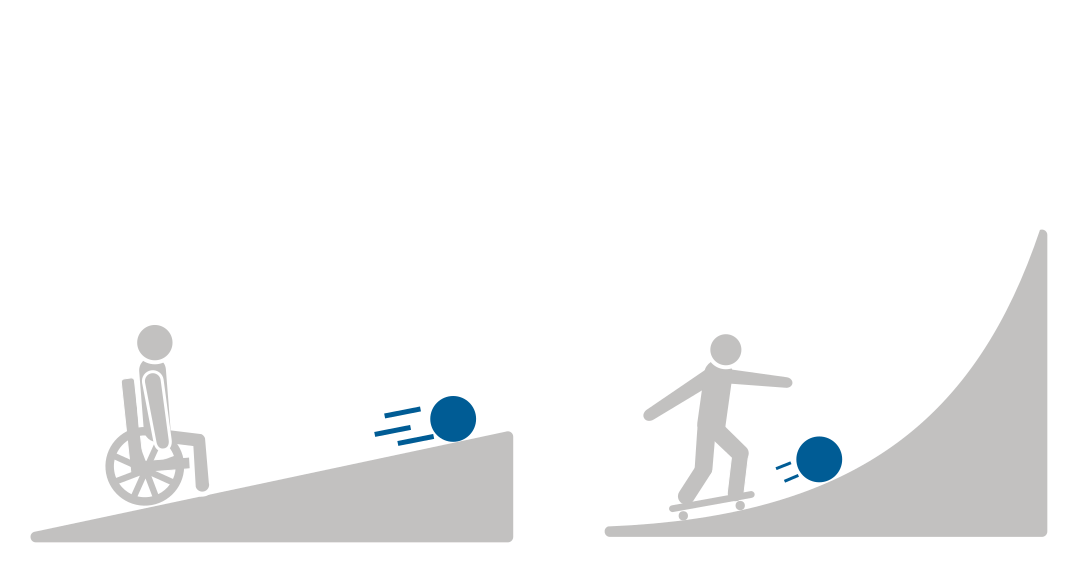
\includegraphics[width=\textwidth]{rampcomparison.png}

Assuming the incline has a constant steepness, the mechanical advantage is equal to the ratio of the length of the inclined plane to the height it rises.

If friction is neglected, the force required to push a weight up the inclined plane is given by:

\[
F_A = \frac{V}{L} F_G
\]

where \( F_A \) is the applied force, \( L \) is the length of the inclined plane, \( V \) is the vertical rise, and \( F_G \) is the gravitational force acting on the mass.

(We haven't yet discussed the sine function, but in case you're familiar with it, note that:

\[
\frac{V}{L} = \sin{\theta}
\]

where \( \theta \) is the angle between the inclined plane and the horizontal surface.)

\begin{Exercise}[title={Ramp}, label=ramp]
A barrel of oil weighs 136 kilograms. You can apply a force of up to 300 newtons. You need to get the barrel onto a platform that is 2 meters high. What is the shortest length of inclined plane you can use?
\end{Exercise}
\begin{Answer}[ref=ramp]
The weight of the barrel is \( 136 \times 9.8 = 1332.8 \) newtons.

Let \( L \) be the length of the inclined plane. The force needed to push the barrel up is related by:

\[
300 = \frac{2}{L} \times 1332.8
\]

Solving for \( L \), we find \( L = \frac{2 \times 1332.8}{300} \approx 8.885 \) meters.
\end{Answer}

\section{Gears}

Gears have teeth that mesh with each other. When you apply torque to one gear, it transfers torque to the other. The resulting torque is increased or decreased depending on the ratio of the number of teeth on the gears.

\includegraphics[width=0.7\textwidth]{gearsNew.png}

If \( N_A \) is the number of teeth on the gear you are turning with a torque of \( T_A \), and \( N_L \) is the number of teeth on the gear it is turning, the resulting torque is:

\[
T_L = \frac{N_A}{N_L} T_A
\]

\begin{Exercise}[title={Gears}, label=gear]
In a bicycle, the goal is not always to gain mechanical advantage, but to spin the pedals slower while applying more force.

You like to pedal your bike at 70 revolutions per minute. The chainring connected to your pedals has 53 teeth. The circumference of your tire is 2.2 meters. You want to ride at 583 meters per minute.

How many teeth should the rear sprocket have?
\end{Exercise}
\begin{Answer}[ref=gear]
The equation relating these quantities is:

\[
583 = 70 \times 2.2 \times \frac{53}{n}
\]

Solving for \( n \), we find \( n = 14 \) teeth.
\end{Answer}

\section{Hydraulics}

In a hydraulic system, such as a car's braking system, you exert force on a piston filled with fluid. The fluid transmits this pressure into another cylinder, where it pushes yet another piston that moves the load.

\includegraphics[width=\textwidth]{hydraulicsNew.png}

The pressure in the fluid is typically measured in pascals (Pa), which is equivalent to \(N / m^2\). We will use pascals for this calculation.

To calculate the pressure you create, divide the force applied by the area of the piston head. To determine the force on the other piston, multiply the pressure by the area of the second piston.

\begin{Exercise}[title={Hydraulics}, label=hydraulics]
Your car has disc brakes. When you apply 2,500,000 pascals of pressure to the brake fluid, the car stops quickly. As the car designer, you want this to require only 12 newtons of force from the driver's foot.

What should the radius of the master cylinder (the piston the driver pushes) be?
\end{Exercise}
\begin{Answer}[ref=hydraulics]
We are solving for the radius \( r \) of the piston. The area of the piston is \( \pi r^2 \), so the pressure is:

\[
\text{Pressure} = \frac{12}{\pi r^2}
\]

Setting the pressure equal to 2,500,000 pascals:

\[
2,500,000 = \frac{12}{\pi r^2}
\]

Solving for \( r \), we find:

\[
r = \sqrt{\frac{12}{\pi \times 2.5 \times 10^6}} \approx 0.00124 \text{ meters}.
\]
\end{Answer}

\graphicspath{{../../Chapters/biases1/en_US}}
\chapter{Cognitivie Biases 1}


Our brains were designed over millions of years by the evolutionary
process. The resulting mind is an amazing and powerful tool, however
not flawless. The human brain has tendencies (or biases) that nudge us
toward bad judgment and poor decisions.

It would be irresponsible to teach you powerful ideas without
also teaching you about the cognitive biases that follow them. There are about 50
that you should know about, but let's start with only a few.

\section{Fundamental Attribution Error}

You tend to attribute
the mistakes of another person to their character, but attribute your
own mistakes to the situation.

Let's say you are at lunch and someone asks you ``Why was Larry late
for class ?''  You are likely to say ``Larry is lazy
and disorganized.''

If someone asks you ``Why were you late for class last week?''  You
are likely to say, ``I don't remember; The class before it must have
run long.''
\includegraphics[width=0.8\textwidth]{bias_late.png}

The solution? Cut people some slack. You probably don't know the whole
story, so assume that their character is as strong as yours.

Or maybe you also need to hold yourself to a higher standard? Do you find
yourself frequently rationalizing your bad judgment, lateness, or
rudeness?  This could be an opportunity for you to become a better
person whose character is stronger regardless of the situation.

\section{Self-Serving Bias}

\newterm{Self-serving bias} is when you blame the situation for your
failures, but attribute your successes to your strengths.

For example, when asked ``Why did you lose the match?'' you are likely
to answer ``The referee wasn't fair.''  When you are asked ``Why did
you win the match?'' you are likely to answer ``Because I have been
training for weeks, and I was very focused.''
\includegraphics[width=0.8\textwidth]{bias_soccer.png}

This bias tends to make us feel better about ourselves, but it makes it
difficult for us to be objective about our strengths and weaknesses.

\section{In-group favoritism}

\newterm{In-group favoritism}: We tend to favor people who are in
a group with us over people who are not in groups with us.

When asked ``Who is the better goalie, Ted or John?''

If Ted is a Star Trek fan like you, you are likely to think he is also
a good goalie.

As you might imagine, this unconscious tendency is the source of a lot
of subtle discrimination based on race, gender, age, and religion.
\includegraphics[width=0.8\textwidth]{bias_group.png}

\section{The Bandwagon Effect and Groupthink}

\newterm{The bandwagon effect} is our tendency to believe the same
things that the people around us believe. This is how fads spread so
quickly: one person buys in, and then the people they know have a
strong tencdency to buy in as well.

\newterm{Groupthink} is similar: To create harmony with the
people around us, we go along with things we disagree with.

It takes a lot of perspective to recognize when those around us are
wrong. And it takes even more courage to openly disagree with them.

\section{The Curse of Knowledge}

Once you know something, you tend to assume everyone else knows it too.

This is why teaching is sometimes difficult: a teacher will assume
that everyone in the audience already knows the same things the
teacher knows.

Also, when we learn that a friend doesn't know something that we know,
we are often very surprised. This surprise can sometimes manifest as
hurtful behavior.

When I find a gap in a friend's knowledge, I try to remind myself that
the friend certainly knows many things that I don't. I also try to
imagine how it would feel if they teased me for my ignorance.

\section{False Consensus}

We tend to believe that more people agree with us than is actually
the case. For example, if you are a member of a particular religion,
you tend to overestimate the percentage of people in the world who are
members of that religion.

When people vote in elections, they are often surprised when their
preferred candidate loses. ``Everyone, and I mean EVERYONE, voted for
Smith!'' they yell.  ``There must have been a mistake in counting the
votes.''

\section{The Spotlight Effect}

You tend to overestimate how much other people are paying attention to
your behavior and appearance.

Think of six people that you talked to today. Can you even remember what
shoes most of them were wearing? Do you care? Do you think any of them
remember which shoes you wore today?

There is an old saying ``You would worry a lot less about how people
think of you, if you realized how rarely they do.''

\section{The Dunning-Kruger Effect}

The less you know, the more confident you are.

When a person doesn't know all the nuance and context in which a question is
asked, the question seems simple. Thus the person tends to be confident in
their answer. As they learn more about the complexity of the space in
which the question lives, they often realize the answer is not nearly so
obvious.

For example, a lot of people will confidently proclaim ``Taxes are too
high! We need to lower taxes.''  An economist who has studied
government budgets, deficits, history, and monetary policy, might say
something like ``Maybe taxes \emph{are} too high. Or maybe they are
too low. Or maybe we are taxing the wrong things. It is a 
complex question.''

When I am talking with people about a particular topic, I do my best
to defer to the person in the conversation who I think has the most
knowledge in the area. If I disagree with the person, I try to figure
out why our opinions are different.

Similarly, you should assume that any opinion that is voiced, specifically, in an
internet discussion is wildly over-simplified. If you really care
about the subject, read a book by a respected expert. Yes, a whole
book -- there are few interesting topics that can be legitimately
explained in less than 100 pages.

\section{Confirmation Bias}

You tend to find and remember information that supports
beliefs you already have. You tend to avoid and dismiss information
that contradicts your beliefs.

If you believe that intelligent creatures have visited from other
planets, you will tend to look for data to support your beliefs. When
you find data that shows that it is just too far for any creature to
travel, you will try to find a reason why the data is incorrect.

Confirmation bias is one reason why people don't change their beliefs
more often.

Confirmation bias wrecks many, many studies. The person doing the
study often has a hypothesis that they believe and very much want to
prove true. It is very tempting to discard data that doesn't support
the hypothesis. Or maybe the person throws all the data away and experiments again and again until they get the result they want.

When you design an experiment, you must describe it explicitly before
you start. You must tell someone: ``If the hypothesis I love is
incorrect, the results will look like this.  If the hypothesis I love
is correct, the results will look like that. And if the results look
any other way, I have neither proved nor disproved the hypothesis.''

Once the experiment is underway, you must not change the plan and you
must not discard any data.

This is scientific integrity. You should demand it from yourself, and
you should expect it from others.

\section{Survivorship bias}

You will pay more attention to those that survived a process than
those who failed.

After looking at a lot of old houses, you might say ``In the 1880s,
they built great houses.'' However, you haven't seen the houses that
were built in the 1880s and didn't survive. Which houses tended to
survive for a long time? Only the great houses -- you are
basing your opinion on a very skewed sample.


\graphicspath{{../../Chapters/buoyancy/en_US}}
\chapter{Buoyancy}

The word buoyancy probably brings to mind images of floating in water. Before we dive in, let's zoom out for a moment and consider that the study of buoyancy is about much more than just boats and water. You might be thinking: I want to be a computer programmer, why do I need to know about buoyancy? This topic is much bigger than it might seem at first glance. Buoyancy concerns how all liquids and gasses interact with gravity. The concept of buoyancy is connected to fundamental concepts about how things work in the universe. The \newterm{buoyant force}, as it’s known in engineering, is an important concept that has wide ranging applications. A big part of engineering is moving stuff around, and understanding buoyancy helps us solve problems where we need to move things in and through fluids. Even if you don't have plans to build a robotic submarine, these are super useful ideas to be familiar with. We’ll start exploring the topic with familiar scenarios around boats and water.

When you put a boat into water, it will sink into the water until
the mass of the water it displaces is equal to the mass of the
boat. We think of this in terms of forces. Gravity pulls the mass of
the boat down. The \newterm{buoyant force} pushes the boat up. A boat
dropped into the water will bob up and down a bit before reaching an
\newterm{equilibrium} where the two forces are equal.
% ADD: Explain Action Reaction Pairs in previous chapter
% ADD: Archimedes principle

The buoyant force pushes things up -- against the force of
gravity. The force is equal to the weight of the fluid being
replaced. So, for example, a cubic meter of freshwater has a mass of
about 1000kg.  If you submerge anything with a volume of one meter in
freshwater on earth, the buoyant force will be about 9800 newtons.

For some things, like a block of styrofoam, this buoyant force will be
sufficient to carry it to the surface. Once it reaches the surface, it
will continue to rise (displacing less water) until the mass of the
water it displaces is equal to its mass. And then we say ``It floats!''

\includegraphics[width=.6\textwidth]{waterDisplacement.png}

For some things, like a block of lead, the buoyant force is not
 sufficient to lift it to the surface, and thus we say ``It sinks!''

This is why a helium balloon floats through the air. The air
that it displaces weighs more than the balloon and the helium itself. (It is easy to forget that air has a mass, but it does.)

\begin{Exercise}[title={Buoyancy}, label=buoyancy]
  You have an aluminum box that has a heavy base, so it will always
  float upright. The box and its contents weigh 10 kg. Its base is 0.3 m x 0.4 m. It is 1m tall.

  When you drop it into freshwater ($1000 kg/m^3$), how far will it sink
  before it reaches equilibrium.\index{equilibrium}

\end{Exercise}
\begin{Answer}[ref=buoyancy]
  Equilibrium will be achieved when the box has displaced 10 kg of water. That is, when it has displaced $0.01$ cubic meters.

  The area of the base of the box is 0.12 square meters.  So if the
  box sinks $x$ meters into the water it will displace $0.12 x$ cubic
  meters.

  Thus at equilibrium $x = \frac{0.01}{0.12} \approx 0.083$ m.  So,
  the box will sink 8.3 cm into the water before reaching equilibrium.
\end{Answer}

\section{The Mechanism of Buoyancy: Pressure}

As you dive down in the ocean, you will experience greater and
greater pressure from the water. And if you take a balloon with you, you
will gradually see it get smaller as the water pressure compresses the
air in the balloon.

Let's say you are 3 meters below the surface of the water. What is the
pressure in Pascals (newtons per square meter)? You can think of the
water as a column of water crushing down upon you. The pressure over
a square meter is the weight of 3 cubic meters of water pressing down.

$$p = (3)(1000)(9.8) = 29,400 \text{ Pa }$$

This is called \newterm{hydrostatic pressure}. The general rule for
hydrostatic pressure in Pascals $p$ is

$p = d g h$

Where  $d$ is the density of the fluid
in kg per cubic meter, $g$ is the acceleration due to gravity in
$m/s^2$, and $h$ is the height of the column of fluid above you.

So, where does buoyant force come from? Basically, the pressure pushing up on the
deepest part of the object is higher than the pressure pushing down on
the shallowest part of the object. That is where bouyancy comes from.

\includegraphics[width=.6\textwidth]{buoyancy.png}

\begin{Exercise}[title={Hydrostatic Pressure}, label=mars_pressure]

  You dive into a tank of olive oil on Mars. How much more
  hydrostatic pressure does your body experience at 5 meters deep than
  it did at the surface?

  The density of olive oil is about 900 kg per square meter. The
  acceleration due to gravity on Mars is 3.721 $m/s^2$.

\end{Exercise}
\begin{Answer}[ref=mars_pressure]
$$p = d g h = (900)(3.721)(5) = 16,744.5 \text{ Pa}$$
\end{Answer}

\section{The Mechanism of Buoyancy: Density}
Notice that although the pressure is increasing as you go deeper, the
buoyant force will \emph{not increase} because the buoyant force is always equal
to the weight of the fluid that is displaced, regardless if that is 1
meter or 100 meters underwater.

Due to the added minerals, saltwater is denser than freshwater. This causes objects float
better in the sea than they do in, say, a river. Lipids, like fats and
oils, are less dense than water, allowing them to float on top of a glass of water.
When you're facing a grease fire, you're told not to put water on it. That's because
the water sinks below the grease, then boils, throwing burning grease everywhere.

\graphicspath{{../../Chapters/heat/en_US}}
\chapter{Introduction to the Kontinua Sequence}

This book will start you on the long and difficult trek to becoming a modern
problem solver. Along the path, you will learn how to use the tools of
math, computers, and science.

Why should you bother? There are big problems in this world that will
require expert problem solvers. Those people will make the world a
better place while enjoying interesting and lucrative careers. We are
talking about engineers, scientists, doctors, computer programmers,
architects, actuaries, and mathematicians. Right now, those occupations represent
about 6\% of all the jobs in the United States. Soon,
that number is expected to rise above 10\%.  On average, people in
that 10\% of the population are expected to have salaries twice that
of their non-technical counterparts.\index{career}

Solving problems is difficult. At some point on this journey, you will
see people who are better at solving problems than you are. You, like
every other person who has gone on this journey, will think ``I have
worked so hard on this, but that person is better at it than
I am. I should quit.'' Don't.\index{quitting}

First, solving problems is like a muscle. The more you do, the better
you get at it.  It is OK to say ``I am not good at this yet.'' That
just means you need more practice.

Second, you don't need to be the best in the world. 10 million people
your age can be better at solving problems than you, \textit{and you
  can still be in the top 10\% of the world}. If you complete this
journey, there will be problems for you to solve and a job where your
problem-solving skills will be appreciated.

\emph{Where do we start?}

The famous physicist Richard Feynman once asked this question: ``If,
in some cataclysm, all of scientific knowledge were to be destroyed,
and only one sentence was passed on to the next generation of
creatures, what statement would contain the most information in the
fewest words?''

His answer was ``All things are made of atoms—little particles that move around in
perpetual motion, attracting each other when they are a little
distance apart, but repelling upon being squeezed into one another.''

\emph{That} seems like a good place to start.

\graphicspath{{../../Chapters/basic_statistics/en_US}}
\chapter{Introduction to the Kontinua Sequence}

This book will start you on the long and difficult trek to becoming a modern
problem solver. Along the path, you will learn how to use the tools of
math, computers, and science.

Why should you bother? There are big problems in this world that will
require expert problem solvers. Those people will make the world a
better place while enjoying interesting and lucrative careers. We are
talking about engineers, scientists, doctors, computer programmers,
architects, actuaries, and mathematicians. Right now, those occupations represent
about 6\% of all the jobs in the United States. Soon,
that number is expected to rise above 10\%.  On average, people in
that 10\% of the population are expected to have salaries twice that
of their non-technical counterparts.\index{career}

Solving problems is difficult. At some point on this journey, you will
see people who are better at solving problems than you are. You, like
every other person who has gone on this journey, will think ``I have
worked so hard on this, but that person is better at it than
I am. I should quit.'' Don't.\index{quitting}

First, solving problems is like a muscle. The more you do, the better
you get at it.  It is OK to say ``I am not good at this yet.'' That
just means you need more practice.

Second, you don't need to be the best in the world. 10 million people
your age can be better at solving problems than you, \textit{and you
  can still be in the top 10\% of the world}. If you complete this
journey, there will be problems for you to solve and a job where your
problem-solving skills will be appreciated.

\emph{Where do we start?}

The famous physicist Richard Feynman once asked this question: ``If,
in some cataclysm, all of scientific knowledge were to be destroyed,
and only one sentence was passed on to the next generation of
creatures, what statement would contain the most information in the
fewest words?''

His answer was ``All things are made of atoms—little particles that move around in
perpetual motion, attracting each other when they are a little
distance apart, but repelling upon being squeezed into one another.''

\emph{That} seems like a good place to start.

\graphicspath{{../../Chapters/stat_spreadsheets/en_US}}
\chapter{Introduction to the Kontinua Sequence}

This book will start you on the long and difficult trek to becoming a modern
problem solver. Along the path, you will learn how to use the tools of
math, computers, and science.

Why should you bother? There are big problems in this world that will
require expert problem solvers. Those people will make the world a
better place while enjoying interesting and lucrative careers. We are
talking about engineers, scientists, doctors, computer programmers,
architects, actuaries, and mathematicians. Right now, those occupations represent
about 6\% of all the jobs in the United States. Soon,
that number is expected to rise above 10\%.  On average, people in
that 10\% of the population are expected to have salaries twice that
of their non-technical counterparts.\index{career}

Solving problems is difficult. At some point on this journey, you will
see people who are better at solving problems than you are. You, like
every other person who has gone on this journey, will think ``I have
worked so hard on this, but that person is better at it than
I am. I should quit.'' Don't.\index{quitting}

First, solving problems is like a muscle. The more you do, the better
you get at it.  It is OK to say ``I am not good at this yet.'' That
just means you need more practice.

Second, you don't need to be the best in the world. 10 million people
your age can be better at solving problems than you, \textit{and you
  can still be in the top 10\% of the world}. If you complete this
journey, there will be problems for you to solve and a job where your
problem-solving skills will be appreciated.

\emph{Where do we start?}

The famous physicist Richard Feynman once asked this question: ``If,
in some cataclysm, all of scientific knowledge were to be destroyed,
and only one sentence was passed on to the next generation of
creatures, what statement would contain the most information in the
fewest words?''

His answer was ``All things are made of atoms—little particles that move around in
perpetual motion, attracting each other when they are a little
distance apart, but repelling upon being squeezed into one another.''

\emph{That} seems like a good place to start.

\graphicspath{{../../Chapters/dc1/en_US}}
\chapter{Introduction to Electricity}

What happens when you turn on a flashlight? The battery in the
flashlight acts as an electron pump. The electrons flow through the
wires to the lightbulb (or LED). As the electrons pass through the
lightbulb, they excite the molecules within, which gives off light and
heat. (LEDs also give off light and heat, but they give off a lot less
heat.) Then the electrons return to the battery to be pumped around
again.

When electricity is flowing through a copper wire, the protons and
neutrons of the copper stay put while the electrons jump between the
atoms on their way from the battery to the lightbulb and back again.

In some materials, like copper and iron, electrons are loosely bound
to their nuclei, forming a sea of electrons, which allows energy to flow. These are good \textit{electrical conductors}. In
other materials, like glass and plastic, electrons don't leave their
nuclei easily. Thus, they are terrible electrical conductors -- we call
them \textit{electrical insulators}. For example, the plastic around a
wire is electrical insulation.

\includegraphics[width=0.8\textwidth]{Insulator_vs_Conductor.png}
% KA: https://www.khanacademy.org/science/physics/electric-charge-electric-force-and-voltage/charge-electric-force/v/conductors-and-insulators

\section{Units}

Electrons are very small, so to study them, scientists came up with a
unit that represents \textit{a lot} of electrons. 1 \textit{coulomb}
is about 6,241,509,074,460,762,608 electrons.  When 5 coulombs enter one end of the wire every second (and simultaneously 5 coulombs exit the other end), we say ``This wire is carrying 5 amperes of current.''\index{coulombs}

(Truthfully, we usually shorten ampere to just ``amp''.  This is
sometimes a little awkward because we often shorten the word
``amplifier'' to ``amp''. You should be able to tell which is which
from the context.)\index{amp or ampere}

If you look at the circuit breakers or fuses for your home's
electrical system, you'll see that each one is rated in amps.  For
example, maybe the circuit that supplies power to your kitchen has a 10
amp circuit breaker. If for some reason, more than 10 amps tries to
pass through that wire, the circuit breaker will turn off the whole
circuit.

When it is on, your flashlight pushes about 1 amp of current
through the lightbulb(When it is off, there is no current in the
lightbulb).

\includegraphics[width=0.8\textwidth]{Circuit_OnOff.png}

The lightbulb creates \textit{Resistance} that the current pushes
through.\index{resistance} Think of it like plumbing: The current is the amount of water
passing through a pipe. The resistance is something that tries to stop
the current -- like a ball of hair. The battery is what allows
 the current to push through the resistance; we call that
pressure \textit{voltage}.\index{voltage}

\section{Circuit Diagrams}

Here is a circuit diagram of your flashlight:

\begin{circuitikz}
\draw (0,0) to[battery1,invert,l=$3V$] ++(0,3)
to [switch,i=1A] ++(3,0)
to [lamp=$1\Omega$,bipoles/length=0.9cm] ++(0,-3) -- (0,0);
\end{circuitikz}

The lines are wires.  The symbols that we  will use:

\begin{tabular}{c c c c}
  Battery & Switch & Lamp & Resistor \\
\begin{circuitikz}
\draw (0,0) to[battery1] (2,0); 
\end{circuitikz}
&
\begin{circuitikz}
\draw (0,0) to[lamp,bipoles/length=0.9cm,l=$3 \Omega$] (2,0); 
\end{circuitikz}
&
\begin{circuitikz}
\draw (0,0) to[switch,/tikz/circuitikz/bipoles/length=1.0cm] (2,0); 
\end{circuitikz}
&
\begin{circuitikz}
\draw (0,0) to[R,  l=$3 \Omega$] (2,0); 
\end{circuitikz} \\
\end{tabular}

The battery pushes the electrons from one end and pulls them back in at the other, so the circuit must go around in a circle for the current to flow. This is why the current stops flowing when the switch breaks the circuit.

You can think of a switch as having zero resistance when it is closed and infinite resistance when it is open.


For our purposes, a lamp is just a resistor that gives off light.
% KA: https://www.khanacademy.org/science/high-school-physics/dc-circuits/electric-power-and-dc-circuits/a/circuit-introduction

\section{Ohm's Law}

Resistance is measured in \textit{ohms}, and we use a Greek capital omega for that: $\Omega$  

Voltage is measured in
\textit{volts}.\index{ohms}\index{volts}

\begin{mdframed}[style=important, frametitle={Ohm's Law}]\index{Ohm's law}
  Whenever a voltage $V$ is pushing a current $I$ through a resistance of $I$, the following is true:

  $$V = IR$$

  where $V$ is in volts, $I$ is in amps, and $R$ is in ohms.
\end{mdframed}
% KA: https://www.khanacademy.org/science/physics/circuits-topic/circuits-resistance/v/circuits-part-1

\section{Power and Watts}

\begin{mdframed}[style=important, frametitle={Joule's Law}]\index{Joule's law}

  When a current $I$ is passing through a resistance $R$, the power consumed is
  
  $$W = I^2 R$$

  where $W$ is in watts, $I$ is in amps, and $R$ is in ohms.
\end{mdframed}

Of course $V = IR$, so we can extend this to:

$$W = I^2 R = I V = \frac{V^2}{R}$$

Your flashlight's batteries provide about 3 volts. How much
battery power is the flashlight using when it is on? The power (in
watts) produced by the battery is the product of the voltage (in
volts) and the current (in amps). So your flashlight is giving off $3
volts \times 1 amp = 3 watts$ of power. Some of that power is given
off as light, some as heat.\index{watts}

A watt is 1 joule of energy per second. We say that a watt is a
measure of \textit{power}.

When we talk about how much energy is stored in a battery, we use a
unit like a kilowatt-hour. A kilowatt-hour is equivalent to 3.6 million
joules.

\section{Another great use of RMS}

In many electrical problems, the voltage fluctuates a lot.  For
example, the fluctuations in voltage makes the sound that comes out of an
audio speaker.

You can use the root-mean-squared of the voltage to figure out the average power
your speaker is consuming.

Let's say that the RMS of the voltage you are sending to the speaker is $V_{rms}$
and the resistance of the speaker is $R$ ohms, then the power consumed
by the speaker is:

$$P = \frac{V_{rms}^2}{R}$$

Similarly, if you know the RMS of the current you are pushing through
the speaker is $I_{rms}$, then the power consumed by the speaker is:

$$P = I_{rms} R$$

\section{Electricity Dangers}

Large amounts of electricity moving through your body can hurt or even kill
you. You must be careful around electricity.

However, your body is not a very good conductor, so low-voltage
systems (like a flashlight) don't have enough voltage to move significant amounts of
current through your body.

However, the  electricity in a power outlet has much more voltage. The voltage
in these outlets is fluctuating between positive and negative, so we
call it \textit{Alternating Current} or AC.
% ADD: Introduce difference between AC and dc

\includegraphics[width=0.8\textwidth]{AC_vs_DC.png}

In most countries, the RMS of the voltage between 110 and 240 V. (The
peak voltage is always $\sqrt{2}$ times the RMS value. In the US, for
example, people say ``Our outlets supply 120 V.'' They mean that the
RMS of the voltage difference between the wire and the earth is 120V.
The peak voltage is almost 170V.)

How much current can a human handle? Not much. You can barely feel 1
mA moving through your body, but at 16 mA, your muscles will clench
and you won't be able to relax them -- many people die from
electrocution because they grab a wire which pushes enough current
through their body to prevent them from letting go of the wire.  At 20
mA, a human's respiratory muscles become paralyzed.

The fuse breaker in a house will often allow 20 A to flow through the
circuit before it shuts off the power: Always, always, always shut off
the power before touching any of the wiring in your house.

While water is actually a mediocre conductor, it can still deliver enough current
to kill you. If you see a wire in a puddle, you should not touch the
puddle. Interestingly, because of the salt, sea water is more than
100 times better at conducting electricity than the water you drink.
% ADD: Sea of electrons makes a good conductor

\includegraphics[width=0.8\textwidth]{Sea_Electrons.png}

If you hold a wire in each hand, how many Ohms of resistance will your
body have? Once it gets past your skin, you will look like a bag of
salt water to the electricity. After the skin, your body will have a
resistance of about 300$\Omega$. However, the skin is a pretty good
insulator. If you have dry, calloused hands, your skin may add a
100,000$\Omega$ to the resistance.

% KA: https://www.khanacademy.org/science/in-in-class10th-physics/in-in-electricity/in-in-electric-power-and-heating-effect-of-current/v/electric-power-energy


\graphicspath{{../../Chapters/dc_circuits/en_US}}
\chapter{Introduction to the Kontinua Sequence}

This book will start you on the long and difficult trek to becoming a modern
problem solver. Along the path, you will learn how to use the tools of
math, computers, and science.

Why should you bother? There are big problems in this world that will
require expert problem solvers. Those people will make the world a
better place while enjoying interesting and lucrative careers. We are
talking about engineers, scientists, doctors, computer programmers,
architects, actuaries, and mathematicians. Right now, those occupations represent
about 6\% of all the jobs in the United States. Soon,
that number is expected to rise above 10\%.  On average, people in
that 10\% of the population are expected to have salaries twice that
of their non-technical counterparts.\index{career}

Solving problems is difficult. At some point on this journey, you will
see people who are better at solving problems than you are. You, like
every other person who has gone on this journey, will think ``I have
worked so hard on this, but that person is better at it than
I am. I should quit.'' Don't.\index{quitting}

First, solving problems is like a muscle. The more you do, the better
you get at it.  It is OK to say ``I am not good at this yet.'' That
just means you need more practice.

Second, you don't need to be the best in the world. 10 million people
your age can be better at solving problems than you, \textit{and you
  can still be in the top 10\% of the world}. If you complete this
journey, there will be problems for you to solve and a job where your
problem-solving skills will be appreciated.

\emph{Where do we start?}

The famous physicist Richard Feynman once asked this question: ``If,
in some cataclysm, all of scientific knowledge were to be destroyed,
and only one sentence was passed on to the next generation of
creatures, what statement would contain the most information in the
fewest words?''

His answer was ``All things are made of atoms—little particles that move around in
perpetual motion, attracting each other when they are a little
distance apart, but repelling upon being squeezed into one another.''

\emph{That} seems like a good place to start.

\graphicspath{{../../Chapters/charge/en_US}}
\chapter{Charge}

If you rub a balloon against your hair and then place it next to a wall it will stick. We
say that it has gotten an \textit{electrical charge}. It stole some
electrons from your hair, and now the ballon has slightly more
electrons than protons. We say that it has a negative electrical
charge.

Objects with slightly more protons than electrons have a positive charge.

This charge is measured in coulombs. The charge of a single proton is
about $1.6 \times 10^{-19}$ coulombs.

An object with a negative charge and an object with a positive charge
will be attracted to each other. Two objects with the same charge will
be repelled by each other.
% ADD: Good place for culloms law
% KA: https://www.khanacademy.org/science/hs-physics/x215e29cb31244fa1:types-of-interactions/x215e29cb31244fa1:coulomb-s-law/v/coulombs-law

\begin{mdframed}[style=important, frametitle={Coulomb's Law}]\index{Coulomb's law}

  If two objects with charge $q_1$ and $q_2$ (in coulombs) are $r$ meters from each other, the force of attraction or repulsion is given by

  $$F = K\frac{\lvert q_1 q_2 \rvert}{r^2}$$

    where $F$ is in newtons and $K$ is Coulomb's constant: about $8.988 \times 10^9$.
  
\end{mdframed}


\begin{Exercise}[title={Coulomb's Law}, label=charged_balloons]

Two balloons are charged with an identical quantity and type of
charge: $-5 \times 10^{-9}$ coulombs. They are held apart at a
separation distance of 12 cm. Determine the magnitude of the
electrical force of repulsion between them. 
  
\end{Exercise}
\begin{Answer}[ref=charged_balloons]

  $$F = K\frac{\lvert q_1 q_2 \rvert}{r^2} = (8.988 \times 10^9) \frac{(-5 \times 10^{-9})(-5 \times 10^{-9})}{0.12^2} = \frac{224.7 \times 10^{-9}}{0.0144} = 15.6 \times 10^{-6}$$

  15.6 micronewtons.
  
\end{Answer}

At this point, you might ask ``If the wall has zero
charge, why is the balloon attracted to it?'' The answer: the
electrons in the wall move away from the balloon. The negative charge
on the balloon pushes electrons into the wall, so the surface of the
wall gets a mild positive charge. The surface is close to the balloon,
so the attraction is stronger than the repulsion.

\includegraphics[width=.5\textwidth]{balloon.png}

\section{Lightning}

A cloud is a cluster of water droplets and ice particles. These
droplets and ice particles are always moving up and down through the
cloud. In this process, electrons get stripped off and end up on the
water droplets at the bottom of the cloud( water droplets collect at the bottom because they are denser). The air between the
droplets is a pretty good insulator, and thus the electrons are reluctant
to jump anywhere. However, eventually, the charge gets so strong that
even the insulating properties of the air is not enough to prevent
the jump, causing lightning.
% ADD: Add water density explanation. ice less dense than liquid water due to crystaline structure.

\includegraphics[width=1\textwidth]{lightning.png}

A lot of lightning moves within a cloud or between clouds. However, a
few jump to the earth. These bolts of lightning vary in the amount of
electrons they carry, but the average is about 15 coulombs.

And thunder occurs because the electrons heat the air they pass through, 
causing the air to expand suddenly, and the resulting shockwave is the sound we know as thunder.
% ADD: Relate speed of light and sound 
\section{But...}

This idea that opposite charges attract creates some heavy questions
that you do not yet have the tools to work with. So the answer is
basically ``Don't ask that question now!''

However, you probably have these questions, so I will point you in
the direction of the answers.

The first is ``In any atom bigger than hydrogen, there are multiple
protons in the nucleus. Why don't the protons push each other out of
the nucleus?''

We aren't ready to talk about it, but there is a force called \textit{the
 nuclear force} which pulls the protons and neutrons in the nucleus
of the atom toward each other. At very, very small distances it is
strong enough to overpower the repulsive force due to the protons'
charges.
% ADD: Effective nuclear charge

Another question is ``Why do the electrons whiz around in a cloud so
far from the nucleus of the atom? Negatively charged electrons should
cling to the protons in the center, right?''

We aren't ready to talk about it, but quantum mechanics tells us that
electrons like to live in a certain specific energy level. Hugging
protons isn't one of those levels.

\graphicspath{{../../Chapters/volume_solids/en_US}}
\chapter{Volumes of Common Solids}


The volume of a rectangular solid is the product of its three
dimensions.  So if a block of ice is 5 cm tall, 3 cm wide and, 2 cm
deep, it's volume is $5 \times 3 \times 2 = 30$ cubic centimeters.

\tdplotsetmaincoords{80}{130} 
\begin{tikzpicture} [scale=1, tdplot_main_coords, axis/.style={->,sdkblue}, 
light vector/.style={-stealth,dashed,very thick, black}, 
vector/.style={-stealth,black,very thick}, 
vector guide/.style={dashed,sdkblue}]

%standard tikz coordinate definition using x, y, z coords
\coordinate (O) at (0,0,0);

%draw axes
\draw[axis] (0,0,0) -- (3,0,0) node[anchor=north east]{$x$};
\draw[axis] (0,0,0) -- (0,4,0) node[anchor=north west]{$y$};
\draw[axis] (0,0,0) -- (0,0,5.2) node[anchor=south]{$z$};

%draw a vector from O to P
\draw[thick,black] (0,0,0) -- (0,0,5);
\draw[thick,black] (0,3,5) -- (0,0,5);
\draw[thick,black] (2,0,5) -- (0,0,5);

\draw[thick,black] (0,0,0) -- (0,3,0);
\draw[thick,black] (0,3,5) -- (0,3,0) node[midway, right]{$5$ cm};
\draw[thick,black] (2,3,0) -- (0,3,0) node[midway, below]{$2$ cm};;

\draw[thick,black] (0,0,0) -- (2,0,0);
\draw[thick,black] (2,0,5) -- (2,0,0);
\draw[thick,black] (2,3,0) -- (2,0,0) node[midway,below]{$3$ cm};

\draw[thick,black] (2,3,5) -- (2,0,5);
\draw[thick,black] (2,3,5) -- (0,3,5);
\draw[thick,black] (2,3,5) -- (2,3,0);

\end{tikzpicture}


A
cubic centimeter is the same as a milliliter. A milliliter of ice
weighs about 0.92 grams.  So the block of ice would have a mass of $30
\times 0.92 = 27.6$ grams. \index{volume ! rectangular solid}

\begin{mdframed}[style=important, frametitle={Volume of a Sphere}]

A sphere with a radius of $r$ has a volume of \index{volume ! sphere}

$$v = \frac{4}{3} \pi r^3$$

(For completeness, the surface area of that sphere would be

$$a  = 4 \pi r^2$$

Note that a circle of radius $r$ is one quarter of ths: $\pi r^2$.)

\end{mdframed}

\begin{Exercise}[title={Flying Sphere}, label=flying_sphere]

An iron sphere is traveling at 5 m/s. (It is not spinning.)  The
sphere has a radius of 1.5 m.  Iron has a density of 7,800 kg per
cubic meter.  How much kinetic energy does the sphere have?
\end{Exercise}
\begin{Answer}[ref=flying_sphere]
  The volume of the sphere (in cubic meters) is

  $$\frac{4}{3}\pi (1.5)^3 = 4.5 \pi \approx 14.14$$

  The mass (in kg) is $14.14 \times 7800 \approx 110,269$

  The kinetic energy (in joules) is

  $$k = \frac{110269 \times 5^2}{2} = 1,378,373$$

  About 1.4 million joules.
\end{Answer}

\section{Cylinders}

The base and the top of a right cylinder are identical circles. The
circles are on parallel planes.  The sides are perpendicular to those
planes.

\tdplotsetmaincoords{75}{0} 
\begin{tikzpicture} [scale=4, tdplot_main_coords, axis/.style={->,sdkblue}]
\draw[dashed, sdkblue] (0.5,0,0) -- (0.5,0,0.7) node[midway, right]{$h$};
\draw[dashed, sdkblue] (0.5,0,0) -- (1,0,0) node[midway, below]{$r$};
\draw[black] (0.5, 0, 0) circle (0.5);
\draw[black] (0.5, 0, 0.7) circle (0.5);
\draw[black] (0,0,0) -- (0,0,0.7);
\draw[black] (1,0,0) -- (1,0,0.7);
\draw[black] (0.5,0,0) circle (0.02);
\draw[black] (0.5,0,0.7) circle (0.02);
\end{tikzpicture}

\begin{mdframed}[style=important, frametitle={Volume of a cylinder}]\index{volume ! right cylinder}


The volume of the a right cylinder of radius $r$ and height
$h$ is given by:

$$v = \pi r^2 h$$

That is, it is the area of the base times the height.

\end{mdframed}

\begin{Exercise}[title={Tablet}, label=tablet]

  A drug company has to create a tablet with volume of 90 cubic millimeters.

  The tablet will be a cylinder with half spheres on each end.  The radius will be 2mm.

  How long do they need to make the tablet to be?

  \vspace{2mm}
  
\tdplotsetmaincoords{90}{20} 
\begin{tikzpicture} [scale=6.5, tdplot_main_coords, axis/.style={->,sdkblue}]
\draw[dashed, sdkblue] (-0.2,0,0) -- (0,0,0);
\draw[dashed, sdkblue] (0,0,0) -- (0,0,0.2) node[midway, right]{2 mm};
\draw[dashed, sdkblue] (0, 0, 0) [x={(0,0,1)}] circle (0.2);
\draw[dashed, sdkblue] (0.5, 0, 0) [x={(0,0,1)}] circle (0.2);
\draw[dashed, sdkblue] (0.5,0,0) -- (0.7,0,0);
\draw[black] (0, 0, -0.2) [y={(0,0,-1)}] arc (90:270:0.2);
\draw[black] (0.5, 0, 0.2) [y={(0,0,-1)}] arc (-90:90:0.2);
\draw[black] (0,0,0.2) -- (0.5,0,0.2);
\draw[black] (0,0,-0.2) -- (0.5,0,-0.2);
\draw[dashed, sdkblue] (-0.2, 0, 0) -- (-0.2, 0, -0.3);
\draw[dashed, sdkblue] (0.7, 0, 0) -- (0.7, 0, -0.3);
\draw[dashed, sdkblue] (-0.2, 0, -0.3) -- (0.7, 0, -0.3) node[midway, below]{?};
\end{tikzpicture}
  

\end{Exercise}
\begin{Answer}[ref=tablet]
  In your mind, you can dissemble the tablet into a sphere (made up of
  the two ends) and a cylinder (between the two ends)
  
  The volume of the sphere (in cubic millimeters) is

  $$\frac{4}{3}\pi (2)^3 =\frac{32}{3}\pi \approx 33.5$$

  Thus the cylinder part has to be $90 - 33.5 = 56.5$ cubic mm. The
  cylinder part has a radius of 2 mm. If the length of the cylinder
  part is $x$, then

  $$\pi 2^2 x = 56.5$$

  Thus $x = \frac{56.5}{4 \pi} \approx 4.5$ mm.

  The cylinder part of the table needs to be 4.5mm.  Thus the entire tablet is 8.5mm long.
  
\end{Answer}

What if the base and top are identical, but the sides aren't
perpendicular to the base? This is called \newterm{oblique cylinder}.

\tdplotsetmaincoords{75}{0} 
\begin{tikzpicture} [scale=4, tdplot_main_coords, axis/.style={->,sdkblue}]
\draw[dashed, sdkblue] (0.7,0,0) -- (0.7,0,0.7) node[midway, right]{$h$};
\draw[dashed, sdkblue] (0.5,0,0) -- (1,0,0) node[midway, below]{$r$};
\draw[black] (0.5, 0, 0) circle (0.5);
\draw[black] (0.7, 0, 0.7) circle (0.5);
\draw[black] (0,0,0) -- (0.2,0,0.7);
\draw[black] (1,0,0) -- (1.2,0,0.7);
\draw[black] (0.5,0,0) circle (0.02);
\draw[black] (0.7,0,0.7) circle (0.02);
\end{tikzpicture}

The volume is still the height times the area of the base.  Note,
however, that the height is measured perpendicular to the bottom and
top. \index{volume ! oblique cylinder}

Why?


\section{Volume, Area, and Height}

On a solid with a flat base, the line that we use to measure height is
always perpendicular to the plane of the base. We can take slices
through the solid that are parallel to that base plane.  For example,
if we have a pyramid with a square base, each slice will be a square
-- small squares near the top, larger squares near the bottom.

\tdplotsetmaincoords{80}{17} 
\begin{tikzpicture} [scale=4, tdplot_main_coords, axis/.style={->,sdkblue}]
  
\draw[dashed, sdkblue] (0.5,0.5,0) -- (0.5,0.5, 1.0) node[midway, right]{$h$};

\draw[black] (0,0,0) -- (0.5,0.5,1.0);
\draw[black] (1,0,0) -- (0.5,0.5,1.0);
\draw[black] (0,1,0) -- (0.5,0.5,1.0);
\draw[black] (1,1,0) -- (0.5,0.5,1.0);

\draw[black] (0,0,0) -- (1,0,0);
\draw[black] (0,0,0) -- (0,1,0);
\draw[black] (1,0,0) -- (1,1,0)node[midway,below]{$w$};
\draw[black] (0,1,0) -- (1,1,0);

\fill[sdkblue,,opacity=0.4] (0.125, 0.125, 0.25) -- (0.875, 0.125, 0.25) -- (0.875, 0.875, 0.25) -- (0.125, 0.875, 0.25);

\draw[dashed,sdkblue] (0.125, 0.125, 0.25) -- (0.875, 0.125, 0.25);
\draw[dashed,sdkblue] (0.125, 0.125, 0.25) -- (0.125, 0.875, 0.25);
\draw[dashed,sdkblue] (0.875, 0.125, 0.25) -- (0.875, 0.875, 0.25);
\draw[dashed,sdkblue] (0.125, 0.875, 0.25) -- (0.875, 0.875, 0.25);

\draw[dashed,sdkblue] (-0.1, -0.1, 0.25) -- (1.1, -0.1, 0.25);
\draw[dashed,sdkblue] (-0.1, -0.1, 0.25) -- (-0.1, 1.1, 0.25);
\draw[dashed,sdkblue] (1.1, -0.1, 0.25) -- (1.1, 1.1, 0.25);
\draw[dashed,sdkblue] (-0.1, 1.1, 0.25) -- (1.1, 1.1, 0.25);

\end{tikzpicture}

We can figure out the area of the slice at every height $z$.  For
example, at $z = 0$ the slice would have area $w^2$.  At $z = h$, the
slice would have zero area.  What about an arbitrary $z$ in between?
The edge of the square would be $w (1 - \frac{z}{h})$.  So the area of
the slice would be $w^2 (1 - \frac{z}{h})^2$

The graph of this would look like this:

\begin{tikzpicture}[scale=5]

\draw [sdkblue,->,thick] (0,0) -- (1.1,0) node[right]{$z$};
\draw [sdkblue,->,thick] (0,0) -- (0,1.1) node[above]{slice area};
\draw [sdkblue,dashed] (1, 1) -- (0,1) node[left] {$w^2$};
\draw [sdkblue,dashed] (1, 1) -- (1,0) node[below] {$h$};
 \fill [sdkblue, opacity=0.4, domain=0:1, variable=\x]
      (0, 0) 
      -- plot ({\x}, {(1.0 - \x)^2})
      -- (1, 0)
      -- cycle;
\draw[thick,draw=black,
      domain=0:1,samples=300,variable=\x] 
      plot (\x,{(1.0 - \x)^2});
\end{tikzpicture}

The volume is given by the area under the curve and above the
axis. Once you learn integration, you will be really good at finding
the area under the curve.  In this case, I will just tell you that in
the picture, the colored region is one third of the rectangle.

Thus, the area of a square-based pyramid is $\frac{1}{3} h w^2$.

In fact:

\begin{mdframed}[style=important, frametitle={Volume of a pyramid}]\index{volume ! pyramid}

  The volume of pyramid whose base has an area of $b$ and height $h$ is given by:

  $$V = \frac{1}{3} h b$$

  Regardless of the shape of the base.
\end{mdframed}

Note that this is true even for oblique pyramids:

\tdplotsetmaincoords{80}{30} 
\begin{tikzpicture} [scale=4, tdplot_main_coords, axis/.style={->,sdkblue}]
  
\draw[dashed, sdkblue] (1.6,0.5,0) -- (1.6,0.5, 1.0) node[midway, right]{$h$};
\fill[sdkblue] (1.6, 0.5, 0) circle (.02);

\draw[black] (0,0,0) -- (1.6,0.5,1.0);
\draw[black] (1,0,0) -- (1.6,0.5,1.0);
\draw[black] (0,1,0) -- (1.6,0.5,1.0);
\draw[black] (1,1,0) -- (1.6,0.5,1.0);

\draw[black] (0,0,0) -- (1,0,0);
\draw[black] (0,0,0) -- (0,1,0);
\draw[black] (1,0,0) -- (1,1,0);
\draw[black] (0,1,0) -- (1,1,0);

\fill[sdkblue,opacity=0.4] (0.4, 0.125, 0.25) -- (1.15, 0.125, 0.25) -- (1.15, 0.875, 0.25) -- (0.4, 0.875, 0.25);

\draw[dashed,sdkblue] (0, -0.1, 0.25) -- (1.3, -0.1, 0.25);
\draw[dashed,sdkblue] (0, -0.1, 0.25) -- (0, 1.1, 0.25);
\draw[dashed,sdkblue] (1.3, -0.1, 0.25) -- (1.3, 1.1, 0.25);
\draw[dashed,sdkblue] (0, 1.1, 0.25) -- (1.3, 1.1, 0.25);

\end{tikzpicture}


\begin{Exercise}[title={Hexagon-based Pyramid}, label=pyramid_volume]

There is a pyramid with a regular hexagon for a base. Each edge is 5 cm long.  The pyramid is 13 cm tall.  What is its volume?

\tdplotsetmaincoords{70}{17} 
\begin{tikzpicture} [scale=.5, tdplot_main_coords]
  
\draw[dashed, sdkblue] (0,0,0) -- (0,0,13) node[right]{13 cm};

\draw[black] (-5,0,0) -- (-2.5,4.33,0) -- (2.5,4.33,0) -- (5,0,0)
-- (2.5, -4.33, 0) -- (-2.5, -4.33,0) -- cycle;

\draw[black] (0, -4.5, 0) node {5 cm};

\draw[black] (-5,0,0) -- (0,0,13);
\draw[black] (0,0,13)--(5,0,0);
\draw[black] (-2.5,4.33,0) -- (0,0,13);
\draw[black] (2.5,4.33,0) -- (0,0,13);
\draw[black] (-2.5,-4.33,0) -- (0,0,13);
\draw[black] (2.5,-4.33,0) -- (0,0,13);
\end{tikzpicture}

\end{Exercise}
\begin{Answer}[ref=pyramid_volume]
  First, you need to find the area of the base, which is a regular hexagon:
  
\begin{tikzpicture}[scale=0.5]
  \draw[black] (-5,0) -- (-2.5,4.33) -- (2.5,4.33) -- (5,0)
-- (2.5, -4.33) -- (-2.5, -4.33) -- cycle node[midway,left]{5 cm};
\draw[sdkblue,dashed] (-5,0) -- (0,0);
\draw[sdkblue,dashed] (5,0) -- (0,0);
\draw[sdkblue,dashed] (-2.5,4.33) -- (0,0);
\draw[sdkblue,dashed] (2.5,4.33) -- (0,0);
\draw[sdkblue,dashed] (-2.5,-4.33) -- (0,0);
\draw[sdkblue,dashed] (2.5,-4.33) -- (0,0);
\end{tikzpicture}

All the angles in this picture are $60^\circ$ or $\frac{\pi}{3}$
radians. Thus, each line is 5 cm long.

Thus, we need to find the area of one of these triangles and multiply that by six.

Every triangle has a base of 5cm. How tall are they?

\begin{tikzpicture}
  \draw[black] (-2.5,0) -- (2.5,0) -- (0,4.33) -- cycle node[midway,left]{5 cm};
  \draw[sdkblue,dashed] (0,0) -- (0,4.33) node[midway,right]{?};
  \draw[black] (-2.0, 0.0) node [right, above] {$60^\circ$};
\end{tikzpicture}

$$5 \sin{60^\circ} = 5\frac{\sqrt{3}}{2}$$

Which is about 4.33 cm.

Thus, the area of single triangle is 

$$\frac{1}{2} (5) \left( 5\frac{\sqrt{3}}{2} \right) = 25 \frac{\sqrt{3}} {4}$$

And the area of the whole hexagon is six times that:

$$75 \frac{\sqrt{3}}{2}$$

Thus, the volume of the pyramid is:

$$\frac{1}{3}h b = \frac{1}{3} 13 \left(75 \frac{\sqrt{3}}{2}\right)$$

About 281.46 cubic centimeters.

\end{Answer}

Note that plotting the area of each slice and finding the area under
the curve will let you find the area of many things.  For example,
let's say that you have a four-sided spiral, where each face has the
same width $w$:

\tdplotsetmaincoords{80}{17} 
\begin{tikzpicture} [scale=4, tdplot_main_coords, axis/.style={->,sdkblue}]

  \def\h{1.570796326794897}
  \def\gap{0.2}
  \def\srad{0.707106781186548}

\fill[sdkblue,opacity=.7] (0,-1,0) -- (-1,0,0) -- (0,1,0) -- (1,0,0) -- cycle;

\draw[black,thick] (0,-1,0) -- (-1,0,0) -- (0,1,0) -- (1,0,0) -- cycle;
\draw[black,thick] (0,-1,\h) -- (-1,0,\h) -- (0,1,\h) -- (1,0,\h) -- cycle;

\foreach \x in {0.0, 0.1, 0.2, 0.3, 0.4, 0.5, 0.6, 0.7, 0.8, 0.9, 1.0, 1.1, 1.2, 1.3, 1.4, 1.5}{
%        \fill[sdkblue, opacity=0.3] ({sin(deg(\x) + 0)},{cos(deg(\x)+ 0)},\x) -- ({sin(deg(\x) + 90)},{cos(deg(\x)+ 90)},\x) --
%        ({sin(deg(\x + \gap) + 90)},{cos(deg(\x + \gap) + 90)},\x + \gap) -- ({sin(deg(\x + \gap) + 0},{cos(deg(\x + \gap)+ 0)},\x + \gap) -- cycle;
        
%        \fill[gray, opacity=0.8] ({sin(deg(\x) + 90)},{cos(deg(\x)+ 90)},\x) -- ({sin(deg(\x) + 180)},{cos(deg(\x)+ 180)},\x) --
%        ({sin(deg(\x + \gap) + 180)},{cos(deg(\x + \gap)+ 180)},\x + \gap) -- ({sin(deg(\x + \gap) + 90)},{cos(deg(\x + \gap)+ 90)},\x + \gap) -- cycle;
        
%        \fill[sdkblue,opacity=0.3] ({sin(deg(\x) + 180)},{cos(deg(\x)+ 180)},\x) -- ({sin(deg(\x) + 270)},{cos(deg(\x)+ 270)},\x) --
%        ({sin(deg(\x + \gap) + 270)},{cos(deg(\x + \gap)+ 270)},\x+\gap) -- ({sin(deg(\x + \gap) + 180)},{cos(deg(\x + \gap)+ 180)},\x + \gap) -- cycle;
        
%        \fill[gray] ({sin(deg(\x) + 270)},{cos(deg(\x)+ 270)},\x) -- ({sin(deg(\x) + 0)},{cos(deg(\x)+ 0)},\x) --
  %        ({sin(deg(\x + \gap) + 0)},{cos(deg(\x + \gap)+0)},\x + \gap) -- ({sin(deg(\x + \gap) + 270)},{cos(deg(\x + \gap)+ 270)},\x +\gap) -- cycle;

  \draw[sdkblue] ({sin(deg(\x) + 0)},{cos(deg(\x)+ 0)},\x) -- ({sin(deg(\x) + 90)},{cos(deg(\x)+ 90)},\x) --
  ({sin(deg(\x) + 180)},{cos(deg(\x)+ 180)},\x) -- ({sin(deg(\x) + 270)},{cos(deg(\x)+ 270)},\x);
      }

\draw[thick,draw=black,
      domain=0:\h,samples=100,variable=\x] 
      plot ({sin(deg(\x) + 0)},{cos(deg(\x)+ 0)}, \x);

\draw[dashed,draw=sdkblue,
      domain=0:\h,samples=100,variable=\x] 
      plot ({\srad * sin(deg(\x) + 45)},{\srad * cos(deg(\x)+ 45)}, \x);

\draw[thick,draw=black,
      domain=0:\h,samples=100,variable=\x] 
      plot ({sin(deg(\x) + 90)},{cos(deg(\x)+ 90)}, \x);
\draw[dashed,draw=sdkblue,
      domain=0:\h,samples=100,variable=\x] 
      plot ({\srad * sin(deg(\x) + 135)},{\srad * cos(deg(\x)+ 135)}, \x);
      
\draw[thick,draw=black,
      domain=0:\h,samples=100,variable=\x] 
      plot ({sin(deg(\x) + 180)},{cos(deg(\x) + 180)}, \x);
%\draw[dashed,draw=sdkblue,
%      domain=0:\h,samples=100,variable=\x] 
%      plot ({\srad * sin(deg(\x) + 225)},{\srad * cos(deg(\x)+ 225)}, \x);

      
\draw[dashed, thick,draw=black,
      domain=0:\h,samples=100,variable=\x] 
      plot ({sin(deg(\x) + 270)},{cos(deg(\x) + 270)}, \x);

%\draw[dashed,draw=sdkblue,
%      domain=0:\h,samples=100,variable=\x] 
%      plot ({\srad * sin(deg(\x) + 315)},{\srad * cos(deg(\x)+ 315)}, \x);


      \fill[sdkblue,opacity=.9] (0,-1,\h) -- (-1,0,\h) -- (0,1,\h) -- (1,0,\h) -- cycle;
      \draw (0.7,-0.6,0) node [below] {$w$};
      \draw[dashed, sdkblue] (-1.1,0,0) -- (-1.1,0,\h) node[midway,left]{$h$};


\end{tikzpicture}

Every slice still has an area of $w^2$,  thus this figure has a volume of $h w^2$.


\begin{Exercise}[title={Volume of a building}, label=building_volume]

An architect is designing a hotel with a right triangular base; the base is 30
meters on each leg.  The building gets narrower as you get closer to
the top, and finally shrinks to a point.  The spine of the building is
where the right angle is. That spine is straight and perpendicular to the ground.

Each floor has a right isosceles triangle as its floor plan.  The
length of each leg is given by this formula:

$$w = 30 \sqrt{1 - \frac{z}{100}}$$

So the width of the building is 30 meters at height $z=0$.  At 100
meters, the building comes to a point.  It will like this:
\hspace{8mm}

\tdplotsetmaincoords{75}{120}
\begin{tikzpicture} [scale=1, tdplot_main_coords]
\def\h{10}
\draw[dashed, sdkblue] (0,3,0) -- (0,3.2,0) -- (0,3.2,\h) node[midway, right]{100m} -- (0,0,\h);

\draw[black] (0,0,0) -- (3,0,0) -- (0,3,0) -- cycle node [midway, above]{30m};
\draw[black] (0,0,0) -- (0,0,\h);
\draw[black] (0.5, 0, 0) -- (0.5, 0.5, 0) -- (0, 0.5, 0);
\draw[thick,draw=black,
      domain=0:\h,samples=100,variable=\x] 
      plot ({3 * sqrt(1 - (\x/\h)}, 0, \x);

\draw[thick,draw=black,
      domain=0:\h,samples=100,variable=\x] 
      plot (0, {3 * sqrt(1 - (\x/\h))}, \x);

\foreach \n in {1,...,\h}{
  \draw [dashed, draw=sdkblue] (0,0,\n) -- ({3 * sqrt(1 - \n/\h)}, 0, \n) -- (0, {3 * sqrt(1 - \n/\h)},\n) -- cycle;
  \draw [draw=sdkblue] (0.5,0,\n) -- (0.5, 0.5, \n) -- (0, 0.5,\n);
};
      
\end{tikzpicture}

What is the volume of the building in cubic meters?
\end{Exercise}
\begin{Answer}[ref=building_volume]

  The area at height $z$ is given by:

  $$a = \frac{1}{2} w^2 =\frac{1}{2} \left(30 \sqrt{1 - \frac{z}{100}}\right)^2 = \frac{1}{2} 900 \left(1 - \frac{z}{100}\right)$$

  If we plot that, it looks like this:

\begin{tikzpicture}
  \def\h{5}
  \draw[sdkblue, ->] (0,0) -- (0, \h + 0.5) node[above] {area};
  \draw[sdkblue, ->] (0,0) -- (3.5, 0) node[right] {$z$};
 \fill [sdkblue, opacity=0.4]
      (0, 0) -- (0,\h) node [left] {$900 m^2$} -- (3,0) node[below] {$100 m$} -- cycle;
\end{tikzpicture}

What is the area of the blue region? $\frac{1}{2} (900)(100) = 45,000$

The building will be 45 thousand cubic meters.


\end{Answer}

\graphicspath{{../../Chapters/angles/en_US}}
\chapter{Introduction to the Kontinua Sequence}

This book will start you on the long and difficult trek to becoming a modern
problem solver. Along the path, you will learn how to use the tools of
math, computers, and science.

Why should you bother? There are big problems in this world that will
require expert problem solvers. Those people will make the world a
better place while enjoying interesting and lucrative careers. We are
talking about engineers, scientists, doctors, computer programmers,
architects, actuaries, and mathematicians. Right now, those occupations represent
about 6\% of all the jobs in the United States. Soon,
that number is expected to rise above 10\%.  On average, people in
that 10\% of the population are expected to have salaries twice that
of their non-technical counterparts.\index{career}

Solving problems is difficult. At some point on this journey, you will
see people who are better at solving problems than you are. You, like
every other person who has gone on this journey, will think ``I have
worked so hard on this, but that person is better at it than
I am. I should quit.'' Don't.\index{quitting}

First, solving problems is like a muscle. The more you do, the better
you get at it.  It is OK to say ``I am not good at this yet.'' That
just means you need more practice.

Second, you don't need to be the best in the world. 10 million people
your age can be better at solving problems than you, \textit{and you
  can still be in the top 10\% of the world}. If you complete this
journey, there will be problems for you to solve and a job where your
problem-solving skills will be appreciated.

\emph{Where do we start?}

The famous physicist Richard Feynman once asked this question: ``If,
in some cataclysm, all of scientific knowledge were to be destroyed,
and only one sentence was passed on to the next generation of
creatures, what statement would contain the most information in the
fewest words?''

His answer was ``All things are made of atoms—little particles that move around in
perpetual motion, attracting each other when they are a little
distance apart, but repelling upon being squeezed into one another.''

\emph{That} seems like a good place to start.

\graphicspath{{../../Chapters/triangles_circles/en_US}}
\chapter{Introduction to the Kontinua Sequence}

This book will start you on the long and difficult trek to becoming a modern
problem solver. Along the path, you will learn how to use the tools of
math, computers, and science.

Why should you bother? There are big problems in this world that will
require expert problem solvers. Those people will make the world a
better place while enjoying interesting and lucrative careers. We are
talking about engineers, scientists, doctors, computer programmers,
architects, actuaries, and mathematicians. Right now, those occupations represent
about 6\% of all the jobs in the United States. Soon,
that number is expected to rise above 10\%.  On average, people in
that 10\% of the population are expected to have salaries twice that
of their non-technical counterparts.\index{career}

Solving problems is difficult. At some point on this journey, you will
see people who are better at solving problems than you are. You, like
every other person who has gone on this journey, will think ``I have
worked so hard on this, but that person is better at it than
I am. I should quit.'' Don't.\index{quitting}

First, solving problems is like a muscle. The more you do, the better
you get at it.  It is OK to say ``I am not good at this yet.'' That
just means you need more practice.

Second, you don't need to be the best in the world. 10 million people
your age can be better at solving problems than you, \textit{and you
  can still be in the top 10\% of the world}. If you complete this
journey, there will be problems for you to solve and a job where your
problem-solving skills will be appreciated.

\emph{Where do we start?}

The famous physicist Richard Feynman once asked this question: ``If,
in some cataclysm, all of scientific knowledge were to be destroyed,
and only one sentence was passed on to the next generation of
creatures, what statement would contain the most information in the
fewest words?''

His answer was ``All things are made of atoms—little particles that move around in
perpetual motion, attracting each other when they are a little
distance apart, but repelling upon being squeezed into one another.''

\emph{That} seems like a good place to start.

\graphicspath{{../../Chapters/pythagorean_theorem/en_US}}
\chapter{Introduction to the Kontinua Sequence}

This book will start you on the long and difficult trek to becoming a modern
problem solver. Along the path, you will learn how to use the tools of
math, computers, and science.

Why should you bother? There are big problems in this world that will
require expert problem solvers. Those people will make the world a
better place while enjoying interesting and lucrative careers. We are
talking about engineers, scientists, doctors, computer programmers,
architects, actuaries, and mathematicians. Right now, those occupations represent
about 6\% of all the jobs in the United States. Soon,
that number is expected to rise above 10\%.  On average, people in
that 10\% of the population are expected to have salaries twice that
of their non-technical counterparts.\index{career}

Solving problems is difficult. At some point on this journey, you will
see people who are better at solving problems than you are. You, like
every other person who has gone on this journey, will think ``I have
worked so hard on this, but that person is better at it than
I am. I should quit.'' Don't.\index{quitting}

First, solving problems is like a muscle. The more you do, the better
you get at it.  It is OK to say ``I am not good at this yet.'' That
just means you need more practice.

Second, you don't need to be the best in the world. 10 million people
your age can be better at solving problems than you, \textit{and you
  can still be in the top 10\% of the world}. If you complete this
journey, there will be problems for you to solve and a job where your
problem-solving skills will be appreciated.

\emph{Where do we start?}

The famous physicist Richard Feynman once asked this question: ``If,
in some cataclysm, all of scientific knowledge were to be destroyed,
and only one sentence was passed on to the next generation of
creatures, what statement would contain the most information in the
fewest words?''

His answer was ``All things are made of atoms—little particles that move around in
perpetual motion, attracting each other when they are a little
distance apart, but repelling upon being squeezed into one another.''

\emph{That} seems like a good place to start.

\graphicspath{{../../Chapters/congruence/en_US}}
\chapter{Introduction to the Kontinua Sequence}

This book will start you on the long and difficult trek to becoming a modern
problem solver. Along the path, you will learn how to use the tools of
math, computers, and science.

Why should you bother? There are big problems in this world that will
require expert problem solvers. Those people will make the world a
better place while enjoying interesting and lucrative careers. We are
talking about engineers, scientists, doctors, computer programmers,
architects, actuaries, and mathematicians. Right now, those occupations represent
about 6\% of all the jobs in the United States. Soon,
that number is expected to rise above 10\%.  On average, people in
that 10\% of the population are expected to have salaries twice that
of their non-technical counterparts.\index{career}

Solving problems is difficult. At some point on this journey, you will
see people who are better at solving problems than you are. You, like
every other person who has gone on this journey, will think ``I have
worked so hard on this, but that person is better at it than
I am. I should quit.'' Don't.\index{quitting}

First, solving problems is like a muscle. The more you do, the better
you get at it.  It is OK to say ``I am not good at this yet.'' That
just means you need more practice.

Second, you don't need to be the best in the world. 10 million people
your age can be better at solving problems than you, \textit{and you
  can still be in the top 10\% of the world}. If you complete this
journey, there will be problems for you to solve and a job where your
problem-solving skills will be appreciated.

\emph{Where do we start?}

The famous physicist Richard Feynman once asked this question: ``If,
in some cataclysm, all of scientific knowledge were to be destroyed,
and only one sentence was passed on to the next generation of
creatures, what statement would contain the most information in the
fewest words?''

His answer was ``All things are made of atoms—little particles that move around in
perpetual motion, attracting each other when they are a little
distance apart, but repelling upon being squeezed into one another.''

\emph{That} seems like a good place to start.

\graphicspath{{../../Chapters/vectors/en_US}}
\chapter{Vectors}

We have talked a some about forces, but in the calculations that we
have done, we have only talked about the magnitude of a force. It is
equally important to talk about its direction. To do the math on
things with a magnitude and a direction (like forces), we need vectors.\index{vectors}

For example, if you jump out of a plane (hopefully with a parachute), 
several forces with different magnitudes and directions will be acting upon 
you. Gravity will push you straight down. That force will be proportional to your weight.
If there were a wind from the west, it would push you toward the east. That force
will be proportional to the square of the speed of the wind and approximately proportional to 
your size. Once you are falling, there will be resistance from the air 
that you are pushing through -- that force will point in the opposite direction
from the direction you are moving and will be proportional to the square of your
speed.
% Image needed

To figure out the net force (which will tell us how we will accelerate), we will 
need to add these forces together. So we need to learn to do math with vectors.

\section{Adding Vectors}

A vector is typically represented as a list of numbers, with each
number representing a particular dimension. For example, if I am
creating a 3-dimensional vector representing a force, it will have
three numbers representing the amount of force in each of the three
axes. For example, if a force of one newton is in the direction of the
$x$-axis, I might represent the vector as $v = [1, 0, 0]$. 
Another vector might be $u = [0.5, 0.9, 0.7]$ \index{vectors!adding}

\tdplotsetmaincoords{80}{130} 
\begin{tikzpicture} [scale=4, tdplot_main_coords, axis/.style={->,sdkblue}, 
vector/.style={-stealth,black,very thick}, 
vector guide/.style={dashed,sdkblue}]

%standard tikz coordinate definition using x, y, z coords
\coordinate (O) at (0,0,0);

%draw axes
\draw[axis] (0,0,0) -- (1.5,0,0) node[anchor=north east]{$x$};
\draw[axis] (0,0,0) -- (0,0.9,0) node[anchor=north west]{$y$};
\draw[axis] (0,0,0) -- (0,0,0.9) node[anchor=south]{$z$};

%draw a vector from O to P
\draw[vector] (O) -- (1,0,0);
\draw[vector] (O) -- (0.5,0.9,0.7);
\draw (0.2,0.0,0.05) node[left] {v};
\draw (0.2,0.35,0.3) node[right] {u};

\draw[vector guide] (0.5,0,0) -- (0.5,0.9,0);
\draw[vector guide] (0.0,0.9,0) -- (0.5,0.9,0);
\draw[vector guide] (0.5,0.9,0) -- (0.5,0.9,0.7);
\end{tikzpicture}

Thinking visually, when we add to vectors, we put the starting point 
second vector at the ending point of the first vector.


\tdplotsetmaincoords{80}{130} 
\begin{tikzpicture} [scale=4, tdplot_main_coords, axis/.style={->,sdkblue}, 
light vector/.style={-stealth,dashed,very thick, black}, 
vector/.style={-stealth,black,very thick}, 
vector guide/.style={dashed,sdkblue}]

%standard tikz coordinate definition using x, y, z coords
\coordinate (O) at (0,0,0);

%draw axes
\draw[axis] (0,0,0) -- (1.5,0,0) node[anchor=north east]{$x$};
\draw[axis] (0,0,0) -- (0,0.9,0) node[anchor=north west]{$y$};
\draw[axis] (0,0,0) -- (0,0,0.9) node[anchor=south]{$z$};

%draw a vector from O to P
\draw[light vector] (0,0,0) -- (0.5,0.9,0.7);
\draw[light vector] (0.5, 0.9, 0.7) -- (1.5, 0.9, 0.7);
\draw[vector] (0,0,0) -- (1.5,0.9,0.7) node[left] {u + v};
\draw (0.7,0.9,0.75) node[left] {v};
\draw (0.2,0.35,0.3) node[right] {u};

\draw[vector guide] (0.5,0,0) -- (0.5,0.9,0);
\draw[vector guide] (0.0,0.9,0) -- (0.5,0.9,0);
\draw[vector guide] (0.5,0.9,0) -- (0.5,0.9,0.7);
\draw[vector guide] (0.5,0.9,0) -- (1.5,0.9,0.0);
\draw[vector guide] (1.5,0.9,0.0) -- (1.5,0.9,0.7);
\draw[vector guide] (1.5,0.0,0.0) -- (1.5,0.9,0.0);

\end{tikzpicture}

If you know the vectors, you will just add them element-wise:

$$ u + v = [0.5, 0.9, 0.7] + [1.0, 0.0, 0.0] = [1.5, 0.9. 0.7] $$

These vectors have 3 components, so we say they are \newterm{3-dimensional}. 
Vectors can have any number of components. For example, the vector
 $[-12.2, 3, \pi, 10000]$ is 4-dimensional.

 You can only add two vectors if they have the same dimension.

 $$ [12, -4] + [-1, 5] = [11,1] $$

 Addition is commutative: If you have two vectors $a$ and $b$, then
 $a + b$ is the same as $b + a$.

 Addition is also associative: If you have three vectors $a$, $b$, and $c$,
 it doesn't matter which order you add them in. 
 That is, $a + (b + c) = (a + b) + c$.

 A 1-dimensional vector is just a number. We say it is a 
 \newterm{scalar}, not a vector.

 \begin{Exercise}[title={Adding vectors}, label=adding_vectors]
Add the following vectors:
\begin{itemize}
    \item $[1, 2, 3] + [4, 5, 6]$
    \item $[-1, -2, -3, -4] + [4, 5, 6, 7]$
    \item $[\pi, 0, 0] + [0, \pi, 0] + [0, 0, \pi]$
\end{itemize}
\end{Exercise}
\begin{Answer}[ref=adding_vectors]
    \begin{itemize}
        \item $[1, 2, 3] + [4, 5, 6] = [5, 7, 9]$
        \item $[-1, -2, -3, -4] + [4, 5, 6, 7] = [3, 3, 3, 3]$
        \item $[\pi, 0, 0] + [0, \pi, 0] + [0, 0, \pi] = [\pi, \pi, \pi]$ 
    \end{itemize}
\end{Answer}

    \begin{Exercise}[title={Adding Forces}, label=adding_forces]
        You are adrift in space. You are near two different stars. 
        The gravity of one star is pulling you towards it with a 
        force of $[4.2, 5.6, 9.0]$ newtons.
        The gravity of the other star is pulling you towards it with
        a force of $[-100.2, 30.2, -9.0]$ newtons. What is the net force?
        \end{Exercise}
        \begin{Answer}[ref=adding_forces]
            To get the net force, you add the two forces:

            $$F = [4.2, 5.6, 9.0] + [-100.2, 30.2, -9.0] = [-96, 35.8, 0.0] \text{ newtons}$$
   
\end{Answer}

\section{Multiplying a vector with a scalar}

It is not uncommon to multiply a vector by a scalar.  For example, a rocket engine
might have a force vector $v$.  If you fire 9 engines in the exact same direction,
the resulting force vector would be $9v$.\index{vectors!multipying by a scalar}

Visually, when we multiply a vector $u$ by a scalar $a$, we get a new vector that
goes in the same direction as $u$ but has a magnitude $a$ times as long as $u$.

\tdplotsetmaincoords{80}{130} 
\begin{tikzpicture} [scale=3, tdplot_main_coords, axis/.style={->,sdkblue}, 
vector/.style={-stealth,black,very thick}, 
vector guide/.style={dashed,sdkblue}]

%standard tikz coordinate definition using x, y, z coords
\coordinate (O) at (0,0,0);

%draw axes
\draw[axis] (0,0,0) -- (1.6,0,0) node[anchor=north east]{$x$};
\draw[axis] (0,0,0) -- (0,2.8,0) node[anchor=north west]{$y$};
\draw[axis] (0,0,0) -- (0,0,1.9) node[anchor=south]{$z$};

%draw a vector from O to P
\draw[vector] (O) -- (0.5,0.9,0.7);
\draw (0.2,0.35,0.3) node[right] {$u$};

\draw[vector] (O) -- (1.5,2.7,2.1) node[right] {$3u$};


\draw[vector guide] (0.5,0,0) -- (0.5,0.9,0);
\draw[vector guide] (0.0,0.9,0) -- (0.5,0.9,0);
\draw[vector guide] (0.5,0.9,0) -- (0.5,0.9,0.7);

\draw[vector guide] (1.5,0,0) -- (1.5,2.7,0);
\draw[vector guide] (0.0,2.7,0) -- (1.5,2.7,0);
\draw[vector guide] (1.5,2.7,0) -- (1.5,2.7,2.1);
\end{tikzpicture}

When you multiply a vector by a scalar, you just multiply each of the components by the scalar:

$$ 3 \times [0.5, 0.9, 0.7] = [1.5, 2.7, 3.6] $$

\begin{Exercise}[title={Multiplying a vector and a scalar}, label=mult_scalar]
    Simplify the following expressions:
    \begin{itemize}
        \item $2 \times [1, 2, 3]$
        \item $[-1, -2, -3, -4] \times -2$
        \item $\pi[\pi, 2\pi, 3\pi]$
    \end{itemize}
    \end{Exercise}
    \begin{Answer}[ref=mult_scalar]
        \begin{itemize}
            \item $2 \times [1, 2, 3] = [2, 4, 6]$
            \item $[-1, -2, -3, -4] \times -3 = [3, 6, 9, 12]$
            \item $\pi[\pi, 2\pi, 3\pi]  = \pi^2, 2\pi^2, 3\pi^2]$ 
        \end{itemize}
    \end{Answer}

Note that when you multiply a vector times a negative number, the new vector points 
in the opposite direction.

\tdplotsetmaincoords{80}{130} 
\begin{tikzpicture} [scale=5, tdplot_main_coords, axis/.style={->,sdkblue}, 
vector/.style={-stealth,black,very thick}, 
vector guide/.style={dashed,sdkblue}]

%standard tikz coordinate definition using x, y, z coords
\coordinate (O) at (0,0,0);

%draw axes
\draw[axis] (0,0,0) -- (0.55,0,0) node[anchor=north east]{$x$};
\draw[axis] (0,0,0) -- (0,0.95,0) node[anchor=north west]{$y$};
\draw[axis] (0,0,0) -- (0,0,0.6) node[anchor=south]{$z$};

%draw a vector from O to P
\draw[vector] (O) -- (0.5,0.9,0.7);
\draw (0.2,0.36,0.3) node[right] {$u$};

\draw[vector] (O) -- (-0.25,-0.45,-0.35) node[right] {$(-0.5)u$};

\draw[vector guide] (0.5,0,0) -- (0.5,0.9,0);
\draw[vector guide] (0.0,0.9,0) -- (0.5,0.9,0);
\draw[vector guide] (0.5,0.9,0) -- (0.5,0.9,0.7);

\draw[vector guide] (-0.25,0,0) -- (-0.25,-0.45,0);
\draw[vector guide] (0,0,0) -- (-0.25,0,0);
\draw[vector guide] (0.0,-0.45,0) -- (-0.25,-0.45,0);
\draw[vector guide] (0,0,0) -- (0,-0.45,0);

\draw[vector guide] (-.25,-0.45,0) -- (-0.25,-0.45,-0.35);
\end{tikzpicture}

\section{Vector Subtraction}

As you might guess, when you subtract one vector from another, 
you just do element-wise subtraction:\index{vectors!subtraction}

$$[4,2,0] - [3,-2, 9] = [1, 4, -9]$$

So, $u - v = u + (-1v)$.

So visually, you reverse the one that is being subtracted:


\tdplotsetmaincoords{80}{130} 
\begin{tikzpicture} [scale=5, tdplot_main_coords, axis/.style={->,sdkblue}, 
light vector/.style={-stealth,dashed,very thick, black}, 
vector/.style={-stealth,black,very thick}, 
vector guide/.style={dashed,sdkblue}]

%standard tikz coordinate definition using x, y, z coords
\coordinate (O) at (0,0,0);

%draw axes
\draw[axis] (0,0,0) -- (0.55,0,0) node[anchor=north east]{$x$};
\draw[axis] (0,0,0) -- (0,1.0,0) node[anchor=north west]{$y$};
\draw[axis] (0,0,0) -- (0,0,0.75) node[anchor=south]{$z$};

%draw a vector from O to P
\draw[light vector] (0,0,0) -- (0.5,0.9,0.7);
\draw[light vector] (0.5, 0.9, 0.7) -- (-0.5, 0.9, 0.7);
\draw[vector] (0,0,0) -- (-0.5,0.9,0.7) node[right] {u - v};
\draw (0.1,0.9,0.75) node[left] {-v};
\draw (0.29,0.34,0.32) node[right] {u};

\draw[vector guide] (0.5,0,0) -- (0.5,0.9,0);
\draw[vector guide] (0.0,0.9,0) -- (0.5,0.9,0);
\draw[vector guide] (0.5,0.9,0) -- (0.5,0.9,0.7);
\draw[vector guide] (0.5,0.9,0) -- (-0.5,0.9,0.0);
\draw[vector guide] (-0.5,0.9,0.0) -- (-0.5,0.9,0.7);
\draw[vector guide] (-0.5,0.0,0.0) -- (-0.5,0.9,0.0);
\draw[vector guide] (0,0.0,0.0) -- (-0.5,0.0,0.0);

\end{tikzpicture}

\section{Magnitude of a Vector}

The \newterm{magnitude} of a vector is just its length. We write the 
magnitude of a vector $v$ as $|v|$.\index{vectors!magnitude of}

We compute the magnitude using the pythagorean theorem.  If $v = [3,4,5]$, 
then

\begin{equation*}
    |v| = \sqrt{3^2 + 4^2 + 5^2} = \sqrt{50} \approx 7.07
\end{equation*}

(You might notice that the notation for the magnitude is exactly like the notation for absolute value.
If you think of a scalar as a 1-dimensional vector, the absolute value and the magnitude are the same. 
For example, the absolute value of -5 is 5.  If you take the magnitude of the one-dimenional vector $[-5]$,
you get $\sqrt{25} = 5$.)

Notice that if you scale up a vector, its magnitude scales by the same amount. For example:

\begin{equation*}
|7[3,4,5]| = 7 \sqrt{50} \approx 7 \times 7.07    
\end{equation*}

The rule then is: If you have any vector $v$ and any scalar $a$:
\begin{equation*}
    |a v| = |a| |v|
\end{equation*}


\begin{Exercise}[title={Magnitude of a Vector}, label=vector_mag]
    Find the magnitude of the following vectors:
    \begin{itemize}
        \item $[1, 1, 1]$
        \item $[-5, -5, -5]$ (that is the same as $-5 \times [1, 1, 1]$)
        \item $[3, 4, -4] + [-2, -3, 5]$
    \end{itemize}
    \end{Exercise}
    \begin{Answer}[ref=vector_mag]
        \begin{itemize}
            \item $|[1, 1, 1]| = \sqrt{3} \approx 1.73 $
            \item $|[-5, -5, -5]| = |-5 \times [1,1,1]| = 5 \sqrt{3} \approx 8.66$
            \item $|[3, 4, 5] + [-2, -3, -4]| = | [1,1,1] | = \sqrt{3} \approx 1.73$ 
        \end{itemize}
    \end{Answer}

\section{Vectors in Python}

NumPy is a library that allows you to work with vectors in Python.  
You might need to install it on your computer. This is done with \pyfunction{pip}. 
\pyfunction{pip3} installs things specifically for Python 3.\index{vectors!in python}

\begin{Verbatim}
pip3 install NumPy
\end{Verbatim}

We can think of a vector as a list of numbers.  
There are also grids of numbers known as \newterm{matrices}. NumPy deals with both in the same way, 
so it refers to both of them as arrays.\index{NumPy}

The study of vectors and matrices is known as \newterm{Linear Algebra}. Some of the functions we need
are in a sublibrary of NumPy called \pyfunction{linalg}. \index{linalg}

As a convention, everyone who uses NumPy, imports it as \textit{np}. \index{np}

Create a file called \filename{first\_vectors.py}:

\begin{Verbatim}
import NumPy as np

# Create two vectors
v = np.array([2,3,4])
u = np.array([-1,-2,3])
print(f"u = {u}, v = {v}")

# Add them
w = v + u
print(f"u + v = {w}")

# Multiply by a scalar
w = v * 3
print(f"v * 3 = {w}")

# Get the magnitude
# Get the magnitude
mv = np.linalg.norm(v)
mu = np.linalg.norm(u)
print(f"|v| = {mv}, |u| = {mu}")
\end{Verbatim}

When you run it, you should see:

\begin{Verbatim}
> python3 first_vectors.py
u = [-1 -2  3], v = [2 3 4]
u + v = [1 1 7]
v * 3 = [ 6  9 12]
|v| = 5.385164807134504, |u| = 3.7416573867739413
\end{Verbatim}

\subsection{Formatting Floats}

The numbers 5.385164807134504 and 3.7416573867739413 are pretty long.  You probably want it 
rounded off after a couple of decimal places.

Numbers with decimal places are called \newterm{floats}. In the placeholder for your float, you 
can specify how you want it formatted, including the number of decimal places.

Change the last line to look like this:\index{floats!formatting}
\begin{Verbatim}
    print(f"|v| = {mv:.2f}, |u| = {mu:.2f}")
\end{Verbatim}

When you run the code, it will be neatly rounded off to two decimal places:
\begin{Verbatim}
|v| = 5.39, |u| = 3.74
\end{Verbatim}

\graphicspath{{../../Chapters/momentum/en_US}}
\chapter{Momentum}

Let's say a 2 kg block of putty is flying through space at 5 meters
per second, and it collides with a larger 3 kg block of putty that is not
moving at all. When the two blocks deform and stick to each other, how
fast will the resulting big block be moving?

Every object has \newterm{momentum}.  The momentum is a vector
quantity: It points in the direction that the object is moving and has
a magnitude equal to its mass times its speed.

Given a set of objects that are interacting, we can sum all their
momentum vectors to get the total momentum.  In such a set, the total
momentum will stay constant.

So, in our example, one object has a momentum vector of magnitude of
10 kg m/s, the other has a momentum of magnitude 0.  Once they have
merged, they have a combined mass of 5 kg.  Thus, the velocity vector
must have magnitude 2 m/s and pointing in the same direction that the
first mass was moving.

\begin{Exercise}[title={Cars on Ice}, label=cars_on_ice]
A car weighing 1000 kg is going north at 12 m/s.  Another car weighing
1500 kg is going east at 16 m/s.  They both hit a patch of ice (with
zero friction) and collide.  Steel is bent and the two objects become
one.  How what is the velocity vector (direction and magnitude) of the
new object sliding across the ice?
\end{Exercise}
\begin{Answer}[ref=cars_on_ice]
  The momentum of the first car is 12,000 kg m/s in the north direction.

  The momentum of the second car is 24,000 kg m/s in the east direction.

  The new object will be moving northeast. What angle is the angle compared with the east?

  $$\theta = \arctan{\frac{12,000}{24,000}} \approx 0.4636 \text{ radians } \approx 26.565\text{ degrees north of east}$$

  The magnitude of the momentum of the new object is $\sqrt{12,000^2 + 24,000^2} \approx 26,833\text{ kg m/s}$

  Its new mass is 2,5000 kg.  So the speed will be $26,833/2,500 = 10.73$ m/s.
\end{Answer}


Notice that kinetic energy ($1/2 m v^2$) is \emph{not} conserved
here.  Before the collision, the moving putty block has $(1/2)(2)(5^2) = 25$
joules of kinetic energy.  Afterward, the big block has $(1/2)(5)(2^2)
= 10$ joules of kinetic energy.  What happened to the energy that was
lost? It was used up deforming the putty.

What if the blocks were marble instead of putty?  Then there would be
very little deforming, so kinetic energy \emph{and} momentum would be
conserved. The two blocks would end up having different velocity
vectors.

Let's assume for a moment that they strike each other straight on, so
there is motion in only one direction, both before and after the
collision.  Can we solve for the speeds of the first block ($v_1$) and
the second block ($v_2$)?

We end up with two equations. Conservation of momentum says:

$$2 v_1 + 3 v_2 = 10$$

Conservation of kinetic energy says:

$$(1/2)(2)(v_1^2) + (1/2)(3)(v_2^2) = 25$$

Using the first equation, we can solve for $v_1$ in terms of $v_2$:

$$v_1 = \frac{10 - 3 v_2}{2}$$

Substituting this into the second equation, we get:

$$\left(\frac{10 - 3 v_2}{2}\right)^2 + \frac{3 v_2^2}{2} = 25$$

Simplifying, we get:

$$v_2^2 - 4 v_2 + 0 = 0$$

This quadratic has two solutions: $v_2 = 0$ and $v_2 = 4$.  $v_2 = 0$
represents the situation before the collision.  Substituting in $v_2 = 4$:

$$v_1 = \frac{10 - 3(4)}{2} = -1$$

Thus, if the blocks are hard enough that kinetic energy is conserved,
after the collision, the smaller block will be heading in the opposite
direction at 1 m/s.  The larger block will be moving at 4 m/s in the
direction of the original motion.

\begin{Exercise}[title={Billiard Balls}, label=billiards]
  
A billiard ball weighing 0.4 kg and traveling at 3 m/s hits a billiard
ball (same weight) at rest. It strikes obliquely so that the ball at rest starts to
move at a 45 degree angle from the path of the ball that hit it.

Assuming all kinetic energy is conserved. How what is the velocity
vector of each ball after the collision?

\end{Exercise}
\begin{Answer}[ref=billiards]

  The original forward momentum was 1.2 kg m/s.  The original kinetic energy is $(1/2)(0.4)(3^2)$ = 1.8 joules. 

  Let $s$ be the post-collision speed of the ball that had been at
  rest.  Let $x$ and $y$ be the forward and sideways speeds
  (post-collision) of the other ball. Conservation of kinetic energy says

  $$(1/2)(0.4)(s^2) + (1/2)(0.4)(x^2+y^2) = 1.8$$

  Forward momentum is conserved:

  $$0.4\frac{s}{\sqrt{2}} + 0.4 x = 1.2$$

  Which can be rewritten:

  $$x = 3 - \frac{s}{\sqrt{2}}$$
  
  Sideways momentum stays zero:

  $$(0.4)\frac{s}{\sqrt{2}} - 0.4 y = 0.0$$

  Which can be rewritten:

  $$y = \frac{s}{\sqrt{2}}$$

  Substituting into to the conservation of kinetic energy equation above:

  $$(1/2)(0.4)(s^2) + (1/2)(0.4)(\left(3 - \frac{s}{\sqrt{2}}\right)^2+\left(\frac{s}{\sqrt{2}}\right)^2 = 1.8$$

  Which can be rewritten:

  $$s^2 - \frac{3}{\sqrt{2}} s + 0 = 0$$

  There are two solutions to this quadratic: $s = 0$ (before collision) and $s = \frac{3}{\sqrt{2}}$. Thus,

  $$y = \frac{3}{2}$$

  and

  $$x = 3 - \frac{3}{2} = \frac{3}{2}$$

  So both balls careen off at $45^\circ$ angles at the exact same speed. 

  
\end{Answer}




\graphicspath{{../../Chapters/dot/en_US}}
\chapter{The Dot Product}
% Reference for diagrams:https://www.mathsisfun.com/algebra/vectors-dot-product.html

If you have two vectors $u = [u_1, u_2, \dots, w_n]$ and $v = [v_1, v_2,\dots, v_n]$ , 
we define the \newterm{dot product} $u \cdot v$ as 
\begin{equation*}
     u \cdot v = (u_1 \times v_1) + (u_2 \times v_2) + \dots + (u_n \times v_n)
\end{equation*} 

So, for example, 
\begin{equation*}
    [2,4, -3] \cdot [5, -1, 1] = 2 \times 5 + 4 \times -1 + -3 \times 1 = 3
\end{equation*}\index{dot product}

This may not seem like a very powerful idea, but dot products are \emph{incredibly} useful. 
The enormous GPUs(Graphics Processing Unit) that let video games render scenes so quickly? 
They primarily function by computing huge numbers of dot products at mind-boggling speeds. 

\begin{Exercise}[title={Basic dot products}, label=dot_products]
    Compute the dot product of each pair of vectors:
    \begin{itemize}
        \item $[1, 2, 3]$, $[4, 5, -6]$
        \item $[\pi, 2\pi]$, $[2, -1]$
        \item $[0,0,0,0]$, $[10,10,10,10]$
    \end{itemize}
\end{Exercise}
\begin{Answer}[ref=dot_products]
        \begin{itemize}
            \item $[1, 2, 3] \cdot [4, 5, -6] = 4 + 10 - 18 = -4$
            \item $[\pi, 2\pi] \cdot [2, -1] = 2\pi - 2\pi = 0$
            \item $[0,0,0,0] \cdot [10,10,10,10] = 0 + 0 + 0 + 0 = 0$ 
        \end{itemize}
\end{Answer}

\section{Properties of the dot product}

Sometimes we need an easy way to say ``The vector of appropriate length is filled with zeros.''
We use the notation $\vec{0}$ to represent this. Then, for any vector $v$, this is true:

$$v \cdot \vec{0} = 0$$

The dot product is commutative:

$$v \cdot u = u \cdot v$$

The dot product of a vector with itself is its magnitude squared:

$$ v \cdot v = |v|^2 $$

If you have a scalar $a$ then:

    $$(v) \cdot (a u) = a (v \cdot u)$$

So, if $v$ and $w$ are vectors that go in the same direction,

    $$v \cdot w = |v| |w|$$

If $v$ and $w$ are vectors that go in opposite directions,

    $$v \cdot w = -|v| |w|$$
    
if $v$ and $w$ are vectors that are perpendicular to each other, their dot product is zero:

  $$ v \cdot w = 0 $$

\section{Cosines and dot products}

Furthermore, dot products' interaction with cosine makes them even more useful is what makes them so useful: 
If you have two vectors $v$ and $u$,

$$v \cdot u = |v| |u| \cos \theta$$

where $\theta$ is the angle between them.

So, for example, if two vectors $v$ and $u$ are perpendicular, the angle between them is $\pi/2$.  
The cosine of $\pi/2$ is 0: The dot product of any two perpendicular vectors is always 0. In fact, if 
the dot product of two non-zero vectors is 0, the vectors \textit{must be} perpendicular.
% diagram needed 

\begin{Exercise}[title={Using dot products}, label=cos_dot_products]
    What is the angle between these each pair of vectors:
    \begin{itemize}
        \item $[1, 0]$, $[0, 1]$
        \item $[3,4]$, $[4,3]$
    \end{itemize}
\end{Exercise}
\begin{Answer}[ref=cos_dot_products]
        \begin{itemize}
            \item $[1,0] \cdot [0,1] = 0$.  The angle must be $\pi/2$.
            \item $[3,4] \cdot [4, 3] = 24$. $|[3,4]| |[4,3]| \cos(\theta) = 24$. 
            $\cos(\theta) = \frac{24}{(5)(5)}$. $\theta = \arccos(\frac{24}{25}) \approx 0.284 \text{ radians}$.
        \end{itemize}
\end{Answer}

If you have two non-zero vectors $v$ and $u$, you can always compute the angle between them:\index{vectors!angle between}

$$\theta = \arccos(\frac{v \cdot u}{|v| |u|})$$
% Breif Description of arccos
\section{Dot products in Python}

NumPy will let you do dot products using the the symbol @.  Open \filename{first\_vectors.py} 
and add the following to the end of the script:

\begin{Verbatim}
    # Take the dot product
    d = v @ u
    print("v @ u =", d)
    
    # Get the angle between the vectors
    a = np.arccos(d / (mv * mu))
    print(f"The angle between u and v is {a * 180 / np.pi:.2f} degrees")    
\end{Verbatim}

When you run it you should get:
\begin{Verbatim}
v @ u = 4
The angle between u and v is 78.55 degrees
\end{Verbatim}

\section{Work and Power}
%diagram here
Earlier, we mentioned that mechanical work is the product of the 
force you apply to something and the amount it moves. For example, if you 
push a train with a force of 10 newtons as it moves 5 meters, you have done 50 joules of work.

What if you try to push the train sideways? That is, it moves down the track 5 meters, 
but you push it as if you were trying to derail it -- perpendicular to its motion.  
You have done no work because the train didn't move at all in the direction you were pushing.

% \includegraphics[width=0.8\textwidth]{train.png}


Now that you know about dot products: The work you do is the dot
product of the force vector you apply and the displacement vector of the train. (The displacement
vector is the vector that tells how the train moved while you pushed it.) \index{work}

Similarly, we mentioned that power is the product of the force you apply and the velocity of the
mass you are applying it to. It is actually the dot product of the force vector and the velocity vector.\index{power}

For example, if you are pushing a sled with a force of 10 newtons and it is moving 2 meters per second, 
but your push is 20 degrees off, you aren't transferring 20 watts of power to the sled.  
You are transferring $10 \times 2 \times \cos(20 \text{ degrees}) \approx 18.8$ watts of power.
%add ramps and sin


\graphicspath{{../../Chapters/functions/en_US}}
\chapter{Functions and Their Graphs}

You can think of a function as a machine: you put something into the
machine, it processes it, and out comes something else, a product. Just as we
often use the variable $x$ to stand in for a number, we often use the
variable $f$ to stand in for a function.
% One of my teachers told me half of understanding math is understanding mathmaticions are just lazy, maybe a good add in somewhere

For example, we might ask, ``Let the function $f$ be defined like this:

\begin{equation*}
f(x) = -5x^2 + 12x + 2
\end{equation*}

What is the value of $f(3)$?''

You would run the number 3 through ``the machine'': $-5(3^2) + 12(3) + 2 = -7$. The answer would be ``$f(3)$ is $7$''.

However, Some functions are not defined for every possible input. For example:

\begin{equation*}
  f(x) = \frac{1}{x}
\end{equation*}

  This is defined for any $x$ except 0, because you can't divide 1 by 0. The set of values that a function can process is called its \textit{domain}.

\begin{Exercise}[title={Domain of a function}, label=function_domain]

  Let the function $f$ be given by $f(x) = \sqrt{x - 3}$.  What is its domain?

\end{Exercise}
\begin{Answer}[ref=function_domain]
  You can only take the square root of nonnegative numbers, so the
  function is only defined when $x - 3 \geq 0$.  Thus the domain is
  all real numbers greater than or equal to 3.
\end{Answer}

\section{Graphs of Functions}

If you have a function, $f$, its graph is the set of pairs $(x, y)$
such that $y = f(x)$.  We usually draw a picture of this set, called a \textit{graph}. 
The graph not only includes the picture, but also the values of x and y used to create it.

Here is the graph of the function $f(x) = -5x^2 + 12x + 2$:

\begin{tikzpicture}
    \begin{axis}[
        xmin=-1,xmax=3.5,
        ymin=-10,ymax=11,
        axis x line=middle,
        axis y line=middle,
        axis line style=<->,
        xlabel={$x$},
        ylabel={$y$},
        ]
        \addplot[no marks,sdkblue,<->] expression[domain=-0.7:3.05,samples=100]{(-5)*(x^2) + (12 * x) + 2}; 
    \end{axis}
\end{tikzpicture}

(Note this is just part of the graph: it goes infinitely in both
directions, remember your vectors.)

Here is the graph of the function $f(x) = \frac{1}{x}$:

\begin{tikzpicture}
    \begin{axis}[
        xmin=-7,xmax=7,
        ymin=-7,ymax=7,
        axis x line=middle,
        axis y line=middle,
        axis line style=<->,
        xlabel={$x$},
        ylabel={$y$},
        ]
        \addplot[no marks,sdkblue,<->] expression[domain=-6.5:-0.15,samples=100]{1/x}; 
        \addplot[no marks,sdkblue,<->] expression[domain=0.15:6.5,samples=100]{1/x}; 
    \end{axis}
\end{tikzpicture}

\begin{Exercise}[title={Draw a graph}, label=draw_graph]

  Let the function $f$ be given by $f(x) = -3x + 3$. Sketch its graph.
% More space needed in exercise box
\end{Exercise}
\begin{Answer}[ref=draw_graph]

  The graph of this function is a line. Its slope is -3.  It intersects the y axis at $(0, 3)$

\begin{tikzpicture}
    \begin{axis}[
        xmin=-1,xmax=3,
        ymin=-7,ymax=7,
        xtick={1},
        ytick={3},
        axis x line=middle,
        axis y line=middle,
        axis line style=<->,
        xlabel={$x$},
        ylabel={$y$},
        ]
        \addplot[no marks,sdkblue,<->] expression[domain=-0.75:2.74,samples=100]{-3 * x + 3}; 
    \end{axis}
\end{tikzpicture}
  
  
\end{Answer}


\section{Can this be expressed as a function?}

Note that not all sets can be expressed as graphs of functions.  For
example, here is the set of points $(x,y)$ such that $x^2 + y^2 = 9$:

\begin{tikzpicture}
    \begin{axis}[
        xmin=-3.5,xmax=3.5,
        ymin=-3.5,ymax=3.5,
        ytick={-3,-2,-1,0,1,2,3},
        axis x line=middle,
        axis y line=middle,
        axis line style=<->,
        xlabel={$x$},
        ylabel={$y$},
        ]
        \addplot[no marks,sdkblue] expression[domain=-3:3,samples=100]{sqrt(9 - x^2)}; 
        \addplot[no marks,sdkblue] expression[domain=-3:3,samples=100]{-1 * sqrt(9 - x^2)}; 
    \end{axis}
\end{tikzpicture}

This cannot be the graph of a function because what would $f(0)$ be? 3
or -3?  This set fails what we call ``the vertical line test'': If any
vertical line contains more than one point from the set, it isn't the graph
of a function.  For example, the vertical line $x = 2$ would cross
the graph twice:
% index vertical line test
\begin{tikzpicture}
    \begin{axis}[
        xmin=-3.5,xmax=3.5,
        ymin=-3.5,ymax=3.5,
        ytick={-3,-2,-1,0,1,2,3},
        axis x line=middle,
        axis y line=middle,
        axis line style=<->,
        xlabel={$x$},
        ylabel={$y$},
        ]
        \addplot[no marks,sdkblue] expression[domain=-3:3,samples=100]{sqrt(9 - x^2)}; 
        \addplot[no marks,sdkblue] expression[domain=-3:3,samples=100]{-1 * sqrt(9 - x^2)};
        \addplot [thick, dashed] coordinates {(2,-2.5)(2,2.5)};

    \end{axis}

\end{tikzpicture}
% include linked exercise: https://youtu.be/xSQFPbhT4Yc


\section{Inverses}

Some functions have inverse functions. If a function $f$ is a machine that turns
number $x$ into $y$, the inverse (usually denoted $f^{-1}$) is the machine that turns $y$ back
into $x$.

For example, let $f(x) = 5x + 1$. Its inverse is
$f^{-1}(x) = (x - 1)/5$. (Spot check it: $f(3) = 16$ and $f^{-1}(16) = 3$)

Does the function $f(x) = x^3$ have an inverse? Yes, $f^{-1}(x) =
\sqrt[3]{x}$. Let's plot the function (solid line) and its inverse (dashed):

\begin{tikzpicture}
    \begin{axis}[
        xmin=-3.5,xmax=3.5,
        ymin=-3.5,ymax=3.5,
        ytick={-3,-2,-1,0,1,2,3},
        axis x line=middle,
        axis y line=middle,
        axis line style=<->,
        xlabel={$x$},
        ylabel={$y$},
        ]
        \addplot[no marks,sdkblue] expression[domain=-3:3,samples=100]{x^3}; 
        \addplot[no marks,sdkblue,dashed] expression[domain=0:3,samples=100]{x^(1/3)}; 
        \addplot[no marks,sdkblue,dashed] expression[domain=-3:0,samples=100]{-1 * (-1 * x)^(1/3)}; 
    \end{axis}
\end{tikzpicture}

The inverse is the same as the function, just with its axes swapped.
This tells us how to solve for an inverse: We swap $x$ and $y$ and
solve for $y$.

For example, if you are given the function $f(x) = 5x + 1$, its graph
is all $(x,y)$ such that $y = 5x + 1$.  The graph of its inverse is
all $(x, y)$ such that $x = 5y + 1$. So you solve for $y$: $y = (x -
1)/5$.

Not every function has an inverse.  For example, $f(x) = x^2$.  Note
that $f(2) = f(-2) = 4$.  What would $f^{-1}(4)$ be? 2 or -2?  This
implies the ``horizontal line test'': If any horizontal line contains
more than one point of a function's graph, that function has no
inverse.
% index horizontal line test
\begin{tikzpicture}
    \begin{axis}[
        xmin=-3.5,xmax=3.5,
        ymin=-1, ymax=6,
        ytick={-1,0,1,2,3,4,5,6},
        axis x line=middle,
        axis y line=middle,
        axis line style=<->,
        xlabel={$x$},
        ylabel={$y$},
        ]
      \addplot[no marks,sdkblue] expression[domain=-3:3,samples=100]{x^2};
      \addplot [thick, dashed] coordinates {(-3,4)(3,4)};
    \end{axis}
\end{tikzpicture}

In some problems, you need an inverse and you don't  need the
whole domain, so you trim the domain to a set you can define an
inverse on. This allow you to make claims such as ``If we restrict the domain to
the nonnegative numbers, the function $f(x) = x^2 - 5$ has an inverse:
$f^{-1}(x) =\sqrt{x + 5}$.

This begs the question: What is the domain of the inverse function $f^{-1}$?

If we let $X$ be the domain of $f$, we can run every member of $X$
through ``the machine'' and gather them in a set on the other
side. This set would be the \textit{image} of the $f$ "machine". (This is the \textit{range} of $f$.)

What is the image of $f(x) = x^2 - 5$? It is the set of all real
numbers greater than or equal to -5. We write this

\begin{equation*}
  \{ x \in {\rm I\!R} | x \geq -5 \}
  \end{equation*}

Now we can say: \textbf{The image of the function is the domain
  of the inverse function.}

In our example, we can use any number greater
than or equal to -5 as input into the inverse function.

\begin{tikzpicture}
    \begin{axis}[
        xmin=-5.5,xmax=7.5,
        ymin=-6, ymax=5,
        xtick={-3, 2},
        ytick={-5, 1},
        axis x line=middle,
        axis y line=middle,
        axis line style=<->,
        ]
      \addplot[no marks,sdkblue, ->] expression[domain=0:3,samples=100]{x^2 - 5} node[right] {$y = x^2 - 5$};
      \addplot [thick, dashed, red, ->] coordinates {(-0.05,-5)(-0.05,4.5)}
      node [draw, red, left, align=left, yshift=-0.6cm, xshift=-0.1cm] {image of $f$ \textit{or}\\ domain of $f^{-1}$};
      \addplot [thick, dashed, blue, ->] coordinates {(-0,-5.1)(6.75,-5.1)}
      node [draw, align=left, above, blue, yshift=0.1cm, xshift=-1.3cm] {domain of $f$ \textit{or}\\image of $f^{-1}$};
    \end{axis}
\end{tikzpicture}


\begin{Exercise}[title={Find the inverse}, label=simple_inverse]

  Let $f(x) = (x - 3)^2 + 2$.  Sketch the graph.

  Using all the real numbers as a domain, does this function have an inverse?

  How would you restrict the domain to make the function invertible?

  What is the inverse of that restricted function?

  What is the domain of the inverse?

\end{Exercise}
\begin{Answer}[ref=simple_inverse]

  This graph is the graph of $y = x^2$ that has been moved to the right by three units and up two units:
 
\begin{tikzpicture}
    \begin{axis}[
        xmin=-1,xmax=7,
        ymin=-1,ymax=7,
        xtick={3, 6},
        ytick={2, 4},
        axis x line=middle,
        axis y line=middle,
        axis line style=<->,
        xlabel={$x$},
        ylabel={$y$},
        ]
      \addplot[no marks,sdkblue,<->] expression[domain=-2.5:6.5,samples=100]{(x - 3)^2 + 2};
      \addplot[dashed] coordinates {(-1, 2)(4,2)};
      \addplot[dashed] coordinates {(3, -1)(3, 3)};
    \end{axis}
\end{tikzpicture}

To prevent any horizontal line from containing more than one point of
the graph, you would need to use the left or the right side: Either
$\{x \in {\rm I\!R}  | x \leq 3\}$ or $\{x {\rm I\!R}| x \geq 3\}$. Most people will choose the
right side; the rest of the solution will assume that you did too.

To find the inverse we swap $x$ and $y$: $x = (y -3)^2 + 2$

The we solve for $y$ to get the inverse: $y = \sqrt{x - 2} + 3$

You can take the square root of nonnegative numbers. So the function
$f^{-1}(x) = \sqrt{x - 2} + 3$ is defined whenever $x$ is greater than
or equal to 2.

\end{Answer}

\section{Graphing Calculators}

One really easy way to understand your function better is to use a graphing
calculator. Desmos is a great, free online graphing calculator. 

In a web browser, go to Desmos: \url{https://www.desmos.com/calculator}

In the field on the left, enter the function $y = x^2 - x - 6$. (For
the exponent, just prefix it with a caret symbol: ``x\^2''.)

\includegraphics[width=0.85\textwidth]{Desmos.png}

\graphicspath{{../../Chapters/falling_bodies/en_US}}
\chapter{Falling Bodies}

Because of gravity, if you throw a hammer straight up in the air, from
the moment it leaves your hand until it hits the ground, it is
accelerating toward the center of the earth at a constant rate.

\includegraphics[width=1\textwidth]{hammerFall.png}

\emph{Acceleration} can be defined as change in velocity. If the hammer leaves your
hand with a velocity of 12 meters per second upward, one second later
it will be rising, and its velocity will have slowed to 2.2 meters per
second. One second after that, the hammer will be falling at a rate of
7.6 meters per second. Every second the hammer's velocity is changing by
9.8 meters per second, and that change is always toward the center of
the earth. When the hammer is going up, gravity is slowing it down by
9.8 meters per second, each second it is in the air.  When the hammer is coming down,
gravity is speeding it up by 9.8 meters per second.\index{acceleration}
% Connect to vectors


\includegraphics[width=.8\textwidth]{hammerTime.png}

Acceleration due to gravity on earth is a constant negative 9.8 meters per second per second:
\begin{equation*}
a = -9.8   
\end{equation*}
(Why is it negative? We are talking about height, which increases as
you go away from the center of the earth. Acceleration is changing the
velocity in the opposite direction.)

\section{Calculating the Velocity}

Given that the acceleration is constant, it makes sense that the
velocity is a straight line. Assuming once again that the hammer
leaves your hand at 12 meters per second, then the upwards velocity at
time $t$ is given by:
\begin{equation*}
  v = 12 - 9.8t
\end{equation*}

Note that the velocity of the hammer is being given as a function. Here is its graph:

\begin{tikzpicture}
    \begin{axis}[
        xmin=-0.25,xmax=2.75,
        ymin=-13,ymax=13,
        axis x line=middle,
        axis y line=middle,
        axis line style=<->,
        xlabel={$t$},
        ylabel={$v$},
        ]
        \addplot[no marks,sdkblue] expression[domain=0:2.25,samples=100]{x * (-9.8) + 12} node[left] {$12 - 9.8t$}; 
    \end{axis}
\end{tikzpicture}

\begin{Exercise}[title={When is the apex of flight?}, label=vapex]
  Given the hammer's velocity is given by $12 - 9.8t$, at what time (in seconds)
  does it stop rising and begin to fall?
\end{Exercise}
\begin{Answer}[ref=vapex]
  Solve for when the velocity is zero.

  $t = \frac{12}{9.8} = 1.22$ seconds after release.
\end{Answer}

At this point, we need to acknowledge air resistance. Gravity
is not the only force on the hammer; as it travels through the air,
the air tries to slow it down. This force is called \emph{air resistance},
and for a large, fast-moving object (like an airplane) it is GIGANTIC force. For a
dense object (like a hammer) moving at a slow speed (what you generate
with your hand), air resistance doesn't significantly affect acceleration.
% Relate to f=ma

\section{Calculating Position}

If you let go of the hammer when it is 2 meters
above the ground, the height of the hammer is given by:
\begin{equation*}
  p = -\frac{9.8}{2}t^2 + 12t + 2
\end{equation*}

Here is a graph of this function:

\begin{tikzpicture}
    \begin{axis}[
        xmin=-1.2,xmax=3.5,
        ymin=-13,ymax=13,
        axis x line=middle,
        axis y line=middle,
        axis line style=<->,
        xlabel={$t$},
        ylabel={$p$},
      ]
      \addplot[no marks,sdkblue,dashed,<-] expression [domain=-0.7:0,samples=100] {(-4.9)*(x^2) + 12 * x + 2};
      \addplot[no marks,sdkblue] expression [domain=0:2.58,samples=100] {(-4.9)*(x^2) + 12 * x + 2};
      \addplot[no marks,sdkblue,dashed,->] expression [domain=2.58:3,samples=100] {(-4.9)*(x^2) + 12 * x + 2};
    \end{axis}
\end{tikzpicture}


How do we know? \textbf{The change in position between time
  $0$ and any time $t$ is equal to the area under the velocity graph
  between $x = 0$ and $x = t$.}

Let's use the velocity graph to figure out how much the position has
changed in the first second of the hammer's flight. Here's the
velocity graph with the area under the graph for the first second filled
in:

\usepgfplotslibrary{fillbetween}

\begin{tikzpicture}
    \begin{axis}[
        xmin=-0.25,xmax=2.75,
        ymin=-13,ymax=13,
        axis x line=middle,
        axis y line=middle,
        axis line style=<->,
        xlabel={$t$},
        ylabel={$v$},
      ]
      \addplot[no marks,sdkblue, name path=f] expression[domain=0:2.25,samples=100]{x * (-9.8) + 12} node[left] {$12 - 9.8t$};
      \path[name path=xaxis] (axis cs:0,0) -- (axis cs:1,0);
      \addplot[
        thick,
        color=sdkblue,
        fill=sdkblue, 
        fill opacity=0.05
    ]
    fill between[
        of=f and xaxis,
        soft clip={domain=0:1},
    ];
    \addplot[dashed,gray] coordinates {(0,12)(1,12)};
    \addplot[dashed,gray] coordinates {(1,12)(1,0)};
    \end{axis}
\end{tikzpicture}

The blue filled region is the area of the dashed rectangle minus that
empty triangle in its upper left.  The height of the rectangle is
twelve and its width is the amount of time the hammer has been in
flight ($t$). The triangle is $t$ wide and $9.8t$ tall. Thus, the
area of the blue region is given by $12t - \frac{1}{2}9.8 t^2$.

That's the change in position. Where was it originally? 2 meters off
the ground. So the height is given by $p = 2 + 12t - \frac{1}{2}9.8t^2$.
We usually write terms so that the exponent decreases, so:

$$p = - \frac{1}{2}9.8t^2 + 12t + 2$$

Finding the area under the curve like this is called
\textit{integration}. We say ``To find a function that gives the
change in position, we just integrate the velocity function.''  A lot
of the study of calculus is learning to integrate different sorts of
functions.\index{integration}

One important note about integration: Any time the curve drops under
the $x$-axis, the area is considered negative. (Which makes sense,
right? If the velocity is negative, the hammer's position is
decreasing.)


\begin{tikzpicture}
    \begin{axis}[
        xmin=-0.25,xmax=2.75,
        ymin=-13,ymax=13,
        axis x line=middle,
        axis y line=middle,
        axis line style=<->,
        xlabel={$t$},
        ylabel={$v$},
      ]
      \addplot[no marks,sdkblue, name path=f] expression[domain=0:2.25,samples=100]{x * (-9.8) + 12} node[left] {$12 - 9.8t$};
      \path[name path=xaxis] (axis cs:0,0) -- (axis cs:2.25,0);
      \addplot[
        thick,
        color=sdkblue,
        fill=sdkblue, 
        fill opacity=0.05
      ]
      fill between[
        of=f and xaxis,
        soft clip={domain=0:1.2245},
      ];
      \addplot[
        thick,
        color=red,
        fill=red, 
        fill opacity=0.07
      ]
      fill between[
        of=f and xaxis,
        soft clip={domain=1.2245:2.1},
      ];
    \end{axis}
\end{tikzpicture}


\section{Quadratic functions}

Functions of the form $f(x) = a x^2 + b x + c$ are called \newterm{quadratic functions}. 
If $a > 0$, the ends go up.
If $a < 0$, the ends go down.\index{quadratic functions}


\begin{tikzpicture}
  \begin{axis}[
      xmin=-2.2,xmax=1.2,
      ymin=-2,ymax=3,
      axis x line=middle,
      axis y line=middle,
      axis line style=<->,
    ]
    \addplot[no marks,sdkblue] expression [domain=-2:1,samples=100] {(2)*(x^2) + 2 * x - 1};
  \end{axis}
  \node[right] at (1,4) {$2x^2 + 2x - 1$};
\end{tikzpicture}
\hspace{4mm}
\begin{tikzpicture}
  \begin{axis}[
    xmin=-1.5,xmax=1.5,
    ymin=-2,ymax=1.5,
    axis x line=middle,
    axis y line=middle,
    axis line style=<->,
  ]
  \addplot[no marks,sdkblue] expression [domain=-1.5:1.5,samples=100] {(-1.2)*(x^2) + 0.5 * x + 1};
\end{axis}
\node[right] at (0.5,1) {$-1.2 x^2 + 0.5 x + 1$};
\end{tikzpicture}

The graph of a quadratic function is a \newterm{parabola}.

\section{Simulating a falling body in Python}

Now you are going to write some Python code that simulates the flying hammer. First, we are just going to print out the position, speed, and acceleration of the hammer for every 1/100th of a second after it leaves your hand. (Later we will make a graph.)

Create a file called \filename{falling.py} and type this into it:

\begin{Verbatim}
# Acceleration on earth
acceleration = -9.8 # m/s/s

# Size of time step
time_step = 0.01 # seconds

# Initial values
speed = 12  # m/s upward
height = 2  # m above the ground
current_time = 0.0  # seconds after release

# Is the hammer still aloft?
while height > 0.0:

    # Show the values
    print(f"{current_time:.2f} s:")
    print(f"\tacceleration: {acceleration:.2f} m/s/s")
    print(f"\tspeed: {speed:.2f} m/s")
    print(f"\theight: {height:.2f} m")

    # Update height
    height = height + time_step * speed

    # Update speed
    speed = speed + time_step * acceleration

    # Update time
    current_time = current_time + time_step


print(f"Hit the ground: Complete")
\end{Verbatim}

When you run it, you will see something like this:
\begin{Verbatim}
0.00 s:
	acceleration: -9.80 m/s/s
	speed: 12.00 m/s
	height: 2.00 m
0.01 s:
	acceleration: -9.80 m/s/s
	speed: 11.90 m/s
	height: 2.12 m
0.02 s:
	acceleration: -9.80 m/s/s
	speed: 11.80 m/s
	height: 2.24 m
0.03 s:
	acceleration: -9.80 m/s/s
	speed: 11.71 m/s
	height: 2.36 m
...
2.60 s:
	acceleration: -9.80 m/s/s
	speed: -13.48 m/s
	height: 0.20 m
2.61 s:
	acceleration: -9.80 m/s/s
	speed: -13.58 m/s
	height: 0.07 m
Hit the ground: Complete
\end{Verbatim}

Note that the acceleration isn't changing at all, but it is changing
the speed, and the speed is changing the height.

We can see that the hammer in our simulation hits the ground just
after 2.61 seconds.

\subsection{Graphs and Lists}

Now, we are going to graph the acceleration, speed, and height using a
library called matplotlib. However, to make the graphs, we
need to gather all the data into lists.\index{matplotlib}

For example, we will have a list of speeds, and the first three
entries will be 12.0, 11.9, and 11.8.\index{lists, python}

We create an empty list and assign it to a variable like this:
\begin{Verbatim}
x = []
\end{Verbatim}

Then we can add items like this:
\begin{Verbatim}
x.append(3.14)
\end{Verbatim}

To get the first time back, we can ask for the object at index 0.
\begin{Verbatim}
y = x[0]
\end{Verbatim}
Note that the list starts at 0.  So if you have 32 items in the list,
the first item is at index 0. The last item is at index 31.

Duplicate the file \filename{falling.py} and name the new copy \filename{falling\_graph.py}

We are going to make a plot of the height over time. At the start of the program, you will import the
matplotlib library.  At the end of the program, you will create a plot and show it to the user.

In \filename{falling\_graph.py}, add the bold code:

\begin{Verbatim}[commandchars=\\\{\}]
\textbf{import matplotlib.pyplot as plt}

# Acceleration on earth
acceleration = -9.8 # m/s/s

# Size of time step
time_step = 0.01 # seconds

# Initial values
speed = 12  # m/s upward
height = 2  # m above the ground
current_time = 0.0  # seconds after release

\textbf{# Create empty lists}
\textbf{accelerations = []}
\textbf{speeds = []}
\textbf{heights = []}
\textbf{times = []}

# Is the hammer still aloft?
while height > 0.0:

    \textbf{# Add the data to the lists}
    \textbf{times.append(current_time)}
    \textbf{accelerations.append(acceleration)}
    \textbf{speeds.append(speed)}
    \textbf{heights.append(height)}
    
    # Update height
    height = height + time_step * speed

    # Update speed
    speed = speed + time_step * acceleration

    # Update time
    current_time = current_time + time_step

\textbf{# Make a plot}
\textbf{fig, ax = plt.subplots()}
fig.suptitle("Falling Hammer")
\textbf{ax.set_xlabel("Time (s)")}
\textbf{ax.set_ylabel("Height (m)")}
\textbf{ax.plot(times, heights)}
\textbf{plt.show()}
\end{Verbatim}

When you run the program, you should see a graph of the height over time.

\includegraphics[width=0.7\linewidth]{heightplot.png}

It is more interesting if we can see all three: acceleration, speed, and height. 
So lets make three stacked plots.  Change the plotting code in \filename{falling\_graph.py} to:\index{matplotlib!subplots}

\begin{Verbatim}
# Make a plot with three subplots
fig, ax = plt.subplots(3,1)
fig.suptitle("Falling Hammer")

# The first subplot is acceleration
ax[0].set_ylabel("Acceleration (m/s/s)")
ax[0].plot(times, accelerations)

# Second subplot is speed
ax[1].set_ylabel("Speed (m/s)")
ax[1].plot(times, speeds)

# Third subplot is height
ax[2].set_xlabel("Time (s)")
ax[2].set_ylabel("Height (m)")
ax[2].plot(times, heights)
plt.show()
\end{Verbatim}

Now you will get plots of all three variables:

\includegraphics[width=0.8\linewidth]{stackedplot.png}

This is what we expected, right?  The acceleration is a constant negative number.  The speed is a
straight line with a negative slope.  The height is a parabola.

A natural question at this point is ``When exactly will the hammer hit the
ground?''  That is, when does $height = 0$? The values of $t$ where a function is zero are
known as its \textit{roots}. Height is given by a quadratic function. In the next
chapter, you will get the trick for finding the roots of any quadratic
function.

\graphicspath{{../../Chapters/solving_quadratics/en_US}}
\chapter{Introduction to the Kontinua Sequence}

This book will start you on the long and difficult trek to becoming a modern
problem solver. Along the path, you will learn how to use the tools of
math, computers, and science.

Why should you bother? There are big problems in this world that will
require expert problem solvers. Those people will make the world a
better place while enjoying interesting and lucrative careers. We are
talking about engineers, scientists, doctors, computer programmers,
architects, actuaries, and mathematicians. Right now, those occupations represent
about 6\% of all the jobs in the United States. Soon,
that number is expected to rise above 10\%.  On average, people in
that 10\% of the population are expected to have salaries twice that
of their non-technical counterparts.\index{career}

Solving problems is difficult. At some point on this journey, you will
see people who are better at solving problems than you are. You, like
every other person who has gone on this journey, will think ``I have
worked so hard on this, but that person is better at it than
I am. I should quit.'' Don't.\index{quitting}

First, solving problems is like a muscle. The more you do, the better
you get at it.  It is OK to say ``I am not good at this yet.'' That
just means you need more practice.

Second, you don't need to be the best in the world. 10 million people
your age can be better at solving problems than you, \textit{and you
  can still be in the top 10\% of the world}. If you complete this
journey, there will be problems for you to solve and a job where your
problem-solving skills will be appreciated.

\emph{Where do we start?}

The famous physicist Richard Feynman once asked this question: ``If,
in some cataclysm, all of scientific knowledge were to be destroyed,
and only one sentence was passed on to the next generation of
creatures, what statement would contain the most information in the
fewest words?''

His answer was ``All things are made of atoms—little particles that move around in
perpetual motion, attracting each other when they are a little
distance apart, but repelling upon being squeezed into one another.''

\emph{That} seems like a good place to start.

\graphicspath{{../../Chapters/drag/en_US}}
\chapter{Drag}

The very first computers were created to do calculations of how
artillery would fly when shot at different angles. The calculations
were similar to the ones you just did for the flying
hammer with two important differences:
\begin{itemize}
\item They were interested in two dimensions: the height and the distance across the ground.
\item However, artillery flies a lot faster than a hammer, so they had to worry about drag from the air.
\end{itemize}
\includegraphics[width=0.8\textwidth]{arrows.png}
\section{Wind resistance}

The first thing they did was put one of the shells in a wind tunnel.
They measured how much force was created when they pushed 1 m/s of
wind over the shell. Let's say it was 0.1 newtons.

One of the interesting things about the drag from the air (often
called \newterm{wind resistance}) is that it increases with the
\emph{square} of the speed. Thus, if the wind pushing on the shell is
3 m/s, instead of 1 m/s, the resistance is $3^2 \times 0.1 = 0.9$
newtons.

(Why? Intuitively, three times as many air molecules are hitting the
shell and each molecule is hitting it three times harder.)

So, if a shell is moving with the velocity vector $v$, the force
vector of the drag points in the exact opposite direction. If $\mu$ is
the force of wind resistance of the shell at 1 m/s, then the magnitude
of the drag vector is $\mu |v|^2$.

\section{Initial velocity and acceleration due to gravity}

Let's say a shell is shot out of a tube at $s$ m/s, and let's say the tube
is tilted $\theta$ radians above level.  Then, the initial velocity
will be given by the vector $[s \cos(\theta), s \sin(\theta)]$

(The velocity of the shell is actually a 3-dimensional vector, but we
are only going to worry about height and horizontal distance; we are
assuming that the operator pointed it in the right direction.)

To figure out the path of the shell, we need to compute its acceleration. We remember that

$$F = m a$$

(Note that $F$ and $a$ are vectors.)  Dividing both sides by $m$ we get:

$$a = \frac{F}{m}$$

So let's figure out the net force on the shell so that we can calculate the acceleration vector.

If the shell has a mass of $b$, the force due to gravity will be in the
downward direction with a magnitude of $9.8 b$ newtons.

To get the net force, we will need to add the force due to gravity
with the force due to wind resistance.

\section{Simulating artillery in Python}

Create a file called \filename{artillery.py}.

\begin{Verbatim}
    import numpy as np
    import matplotlib.pyplot as plt
    
    # Constants
    mass = 45 # kg
    start_speed = 300.0 # m/s
    theta = np.pi/5 # radians (36 degrees above level)
    time_step = 0.01 # s
    wind_resistance = 0.05 # newtons in 1 m/s wind
    force_of_gravity = np.array([0.0, -9.8 * mass]) # newtons
    
    # Initial state
    position = np.array([0.0, 0.0]) # [distance, height] in meters
    velocity = np.array([start_speed * np.cos(theta), start_speed * np.sin(theta)])
    time = 0.0 # seconds
    
    # Lists to gather data
    distances = []
    heights = []
    times = []
    
    # While shell is aloft
    while position[1] >= 0:
        # Record data
        distances.append(position[0])
        heights.append(position[1])
        times.append(time)
    
        # Calculate the next state
        time += time_step
        position += time_step * velocity
    
        # Calculate the net force vector
        force = force_of_gravity - wind_resistance * velocity**2
    
        # Calculate the current acceleration vector
        acceleration = force / mass
    
        # Update the velocity vector   
        velocity += time_step * acceleration
    
    print(f"Hit the ground {position[0]:.2f} meters away at {time:.2f} seconds.")
    
    # Plot the data
    fig, ax = plt.subplots()
    ax.plot(distances, heights)
    ax.set_title("Distance vs. Height")
    ax.set_xlabel("Distance (m)")
    ax.set_ylabel("Height (m)")
    plt.show()        
\end{Verbatim}

When you run it, you should get a message like:
\begin{Verbatim}
Hit the ground 1696.70 meters away at 20.73 seconds.
\end{Verbatim}

You should also see a plot of the shell's path:

\includegraphics[width=0.8\textwidth]{artillery.png}

\section{Terminal velocity}

If you shot the shell very, very high in the sky, it would keep accelerating 
toward the ground until the force of gravity and the force of the wind resistance were equal.
The speed at which this happens is called the \newterm{terminal velocity}.  The terminal velocity of a
falling human is about 53 m/s.

\begin{Exercise}[title={Terminal velocity}, label=terminal_velocity]
    What is the terminal velocity of shell described in our example?
\end{Exercise}
\begin{Answer}[ref=terminal_velocity]
The force of gravity is $9.8 \times 45 = 441$ newtons.

At any speed $s$, the force of wind resistance is $0.05 \times s^2 = 0.05 s^2$ newtons.

At terminal velocity, $0.05 s^2 = 441$. 

Solving for $s$, we get $s = \sqrt{\frac{441}{0.05}}$

Thus, terminal velocity should be about 94 m/s.

\end{Answer}

\graphicspath{{../../Chapters/vector_functions/en_US}}
\chapter{Introduction to the Kontinua Sequence}

This book will start you on the long and difficult trek to becoming a modern
problem solver. Along the path, you will learn how to use the tools of
math, computers, and science.

Why should you bother? There are big problems in this world that will
require expert problem solvers. Those people will make the world a
better place while enjoying interesting and lucrative careers. We are
talking about engineers, scientists, doctors, computer programmers,
architects, actuaries, and mathematicians. Right now, those occupations represent
about 6\% of all the jobs in the United States. Soon,
that number is expected to rise above 10\%.  On average, people in
that 10\% of the population are expected to have salaries twice that
of their non-technical counterparts.\index{career}

Solving problems is difficult. At some point on this journey, you will
see people who are better at solving problems than you are. You, like
every other person who has gone on this journey, will think ``I have
worked so hard on this, but that person is better at it than
I am. I should quit.'' Don't.\index{quitting}

First, solving problems is like a muscle. The more you do, the better
you get at it.  It is OK to say ``I am not good at this yet.'' That
just means you need more practice.

Second, you don't need to be the best in the world. 10 million people
your age can be better at solving problems than you, \textit{and you
  can still be in the top 10\% of the world}. If you complete this
journey, there will be problems for you to solve and a job where your
problem-solving skills will be appreciated.

\emph{Where do we start?}

The famous physicist Richard Feynman once asked this question: ``If,
in some cataclysm, all of scientific knowledge were to be destroyed,
and only one sentence was passed on to the next generation of
creatures, what statement would contain the most information in the
fewest words?''

His answer was ``All things are made of atoms—little particles that move around in
perpetual motion, attracting each other when they are a little
distance apart, but repelling upon being squeezed into one another.''

\emph{That} seems like a good place to start.

\graphicspath{{../../Chapters/fertilizer/en_US}}
\chapter{Fertilizer}

FIXME 
First, Allison has learned she does not need a colon after FM

\textit{Here are some thoughts on expanding the introduction to the Fertilizer Chapter. This might be a good moment to discuss the multidisciplinary nature of Kontinua. 
In a regular science class I'm guessing you wouldn't get electricity and Fertilizer in the same textbook. Why is there a chapter on Fertilizer here? Are you introducing us to the major ways science has given us more power and allowed population to grow? Can we discuss your thoughts on why problem solvers need a basic understanding of Fertilizer and I'll write up a new introduction to this chapter based on the discussion?}

\textit{What do you think about adding a conclusion that talks about the connection between fertilizer (nitrogen), dynamite and the origin of the Nobel peace prize? I know you don't want too much history and philosophy but this seems like a great moment to add a little narrative spice}.

Chapter text starts here: 


In 1950, there were 2.5 billion people on the planet, and about 65\%
were malnourished. In 2019, there were 7.7 billion people on the
planet, and only 15\% are malnourished. How did crop yields increase
so much? There were several factors: better crop varieties,
reliable irrigation, increased mechanization, and affordable fertilizers.\index{fertilizer}

When a plant grows, it takes molecules out of the soil and uses them
to build proteins. It primarily needs the elements nitrogen ($N$),
phosphorus ($P$), and potassium ($K$).\index{nitrogen} \index{phosphorus} \index{potassium}

When you buy a bag of fertilizer at the store, it typically has
three numbers on the front.  For example, you might buy a bag of
``24-22-4''.  This means that 24\% of the mass of the bag is nitrogen,
22\% is phosphorus, and 4\% is potassium.

Potassium comes as potassium carbonate ($K_2CO_3$), potassium chloride
($KCl$), potassium sulfate ($K_2 SO_4$), and potassium nitrate
($KNO_3$). Any blend of these chemicals is known as ``potash''. Potash
is dug up out of mines. \index{potash}

Phosphorus is also mined, but is refined into phosphoric acid
($H_3PO_4$) before it is put into fertilizer.

Nitrogen is an especially interesting case for 2 reasons:
\begin{itemize}
\item Worldwide farmers apply more nitrogen to their soil than potassium or phosphorous combined.
\item 78\% of the air we breathe is nitrogen in the form of $N_2$, but
  neither plants nor animals can utilize nitrogen in that form.
\end{itemize}

\section{The Nitrogen Cycle}

Converting the $N_2$ in the air into a form that a plant can use
is known as \newterm{nitrogen fixation}. For billions of years, there
were only two ways that nitrogen fixation occurred on earth:
\begin{itemize}
\item The energy from lightning causes $N_2$ and $H_2O$ to reconfigure as ammonia ($NH_3$) and nitrate ($NO_3$). This accounts for about 10\% of all naturally occurring nitrogen fixation.
\item Cyanobacteria are responsible for the rest. They convert $N_2$ into ammonia.
\end{itemize}\index{nitrogen cycle} \index{nitrogen fixation}

Let's say that you are eating soybeans. There is a cyanobacteria
called \newterm{rhizobia} that has a symbiotic relationship with
soybean plants.  Rhizobia fixes nitrogen for the soybean plant. The
soybean plant performs photosynthesis and gives sugars to the
rhizobia.

The proteins in the soybeans contain nitrogen from the rhizobia. When
you eat them, you use some of the nitrogen to build new proteins. You
probably don't use all the nitrogen, so your cells release ammonia into your blood.

Ammonia likes to react with things, so your liver combines the ammonia
with carbon dioxide to make urea ($CO(NH_2)_2$).  Your kidneys take
the urea out of your blood and mix it with a bunch of water and salts
in your bladder.  When you urinate, the urea leaves your body.\index{urea}

If you urinate on the ground, the nearby plants can take the nitrogen out of
the urea.\index{urine}

When you die, the nitrogen in your proteins will return to the soil as
ammonia and nitrate.

For centuries, farms got their nitrogen from urine, feces, and rotting
organic material. There were two challenges with this:
\begin{itemize}
\item Human pathogens had to be kept away from human food.
\item There was simply not enough to support 7.7 billion people.
\end{itemize}

So we had to figure out how to do nitrogen fixation at an industrial
level.

\section{The Haber-Bosch Process}

During World War I, two German scientists, Fritz Haber and Carl Bosch
figured out how to make ammonia from $N_2$ and $H_2$ using high
temperatures and pressures. This is how nearly all nitrogen fertilizer
is created today.\index{Haber-Bosch process}

Where do we get the $H_2$? From methane ($CH_4$) in natural gas. Today, 3-5\%
of the world's natural gas production is consumed in the Haber-Bosch
process.

The ammonia is converted into ammonium nitrate ($NH_4NO_3$) or urea
before it is shipped to farms.

\section{Other nutrients}

Healthy plants require several other elements that are sometimes
applied as fertilizer: calcium, magnesium, and sulfur.

Finally, tiny amounts of copper, iron, manganese, molybdenum, zinc, and
boron are sometimes needed.

\graphicspath{{../../Chapters/concrete/en_US}}
\chapter{Concrete}

To make concrete, you mix cement with water and an aggregate (sand or
rock).  The cement is usually only about 10 to 15 percent of the
mixture. The cement reacts with the water, and the resulting solid
binds the aggregate together. In 2019, the world consumed 4.5 billion
tons of cement.\index{concrete} \index{cement}

Concrete is hard and durable. The mortar between the pyramids at Giza
is concrete -- it is now 5000 years old. Today we use concrete to
build many structures including buildings, bridges, airport runways,
and dams.

There are many kinds of cement, but the most common is Portland
cement. It is made by heating limestone (calcium carbonate) with clay
(for silicon) in a kiln. Two things come out of the kiln: Carbon
dioxide and a hard substance called ``clinker''.  The clinker is
ground up with some gypsum before it is sent to market.

The carbon dioxide is released into the atmosphere. Cement manufacture
is responsible for about 8\% of the world's $CO_2$ emissions; it is a
major contributor to climate change.

Really hard concrete, like that used in a nuclear power plant, can
support 3,000 kg per centimeter without being crushed.  However, if
you pull on two ends of a piece of concrete it comes apart pretty
easily. We say that concrete can handle a lot of \newterm{compressive
  stress}, but not much \newterm{tensile} stress.

\section{Steel reinforced concrete}

Many places where we use concrete (like in a bridge), we need both
compressive and tensile stress.  Often the top of a beam is undergoing
compression and the bottom of the beam is undergoing tension.

FIXME Picture here

Steel has tremendous tensile strength, but not as much compressive
strength as concrete. To get both tensile \emph{and} compressive
strength, we often bury steel bars or cables inside the concrete.
This is known as \newterm{steel-reinforced concrete}. The concrete
generally does a very good job protecting the steel, which keeps it
from rusting.\index{steel reinforced concrete}

You may have heard of \newterm{rebar}.  That is just short for
``reinforcing bar''.  Typically rebar has bumps and ridges that keep
the bar and the concrete from moving independently.\index{rebar}

\section{Recycling concrete}

A lot of concrete structures only last about 100 years. When they are
demolished, the concrete can be reused as aggregate in other projects.
Often the concrete bits are mixed with cement and made into concrete again.

If the concrete to be reused is reinforced with steel, the steel has
to be removed and recycled separately.  Then the concrete is crushed
into small pieces.

\graphicspath{{../../Chapters/metals/en_US}}
\chapter{Metals}

Elements that transmit electricity well, even at low temperatures, are
called \newterm{metals}. Here are some metals that you are probably familiar
with: aluminum, iron, copper, tin, gold, silver, and platinum. Aluminum and
iron are particularly common; together they make up about 14\% of the
earth's crust.

An \newterm{alloy} is a mixture of elements that includes at least one
metal. Brass, for example, is an alloy of copper and zinc.  Bronze is
an alloy of copper and tin.

\section{Steel}

One of the most common alloys is steel, an alloy of iron and carbon.
In pure iron, the molecules slip easily past each other, so pure iron
is relatively soft and easily deformed. The carbon in steel prevents
that slipping, thus steel is much, much harder than iron.

How much carbon? If you put less than 0.002\% by weight, you end up
with something very much like pure iron.  As you increase the carbon,
it gets harder and harder.  Once it gets above about 2\%, the result
is very brittle.

If you add about 11\% chromium to steel, you get \newterm{stainless
  steel} which resists rusting.

\begin{Exercise}[title={Tensile Strength}, label=tensile-mpa]

The tensile strength of steel is usually between 400 MPa and 1200
MPa. A Mega Pascal (MPa) is the strength necessary to hold 1,000,000 newtons of
force with a cable that has a 1 square meter cross section. Or,
equivalently, to hold 1 newton of force with a cable that has a 1
square millimeter cross section. 

If you have are buying a round cable that has a tensile strength of
700 Mpa and must hold a 100 kg man aloft, what the diameter of the
smallest cable you can use?
  
\end{Exercise}
\begin{Answer}[ref=tensile-mpa]
On earth, holding a 100 kg man aloft requires 980 Newtons of force.

$980/700 = 1.4$, so you need a cable with a cross-section area of 1.4
square millimeters.

$$\pi r^2 = 1.4$$

So $r = \sqrt{1.4/\pi} \approx .67$ millimeters.  So the cable would
have to have a diameter of at least 1.34 millimeters.

\end{Answer}

Here are some approximate tensile strengths of ather materials:

\begin{tabular}{c|c}
  Material & Tensile strength (MPa) \\
  \hline
  Iron & 3 \\
  Concrete & 4 \\
  Rubber & 16 \\
  Glass & 33 \\
  Wood & 40 \\
  Nylon & 100 \\
  Human hair & 200 \\
  Aluminum  & 300 \\
  Steel & 700 \\
  Spider webs & 1000 \\
  Carbon fiber & 4000
\end{tabular}

\section{What metal for what task?}

You will see copper used a lot for electrical wires in your house and
appliances because it is very efficient at moving electricity (very
little power is lost as heat). It is also very good a transmitting
heat, so you will often see copper pots and pans.

Aluminum is less dense than copper, and is still a pretty good
conductor of electricity. Thus, the overhead wires in a power system
are often made of aluminum.

Aluminum is not as strong as steel, but considerably lighter. It is
often used structurally where weight is a concern: skyscrapers, cars,
airplanes, and ships.

Titanium is about as strong as steel, but it weights about half as
much. Titanium is very difficult to work with, so it is used in places
where weight and strength are very important and cost is not:
airplanes and bicycles.

(Carbon fiber, which is light, strong, and very easy to work with, is
replacing aluminum and titanium in many applications. 20 years ago,
many expensive bicycles were made of titanium. These days the vast
majority are made with carbon fiber.)

Zinc and tin are very resistant to corrosion, so they are often used
as a coating to prevent steel from rusting. They are also used in many
alloys for the same reason.  In the United States, the penny is 97.5\%
zinc and only 2.5\% copper.


\graphicspath{{../../Chapters/basic_spreadsheet/en_US}}
\chapter{Introduction to the Kontinua Sequence}

This book will start you on the long and difficult trek to becoming a modern
problem solver. Along the path, you will learn how to use the tools of
math, computers, and science.

Why should you bother? There are big problems in this world that will
require expert problem solvers. Those people will make the world a
better place while enjoying interesting and lucrative careers. We are
talking about engineers, scientists, doctors, computer programmers,
architects, actuaries, and mathematicians. Right now, those occupations represent
about 6\% of all the jobs in the United States. Soon,
that number is expected to rise above 10\%.  On average, people in
that 10\% of the population are expected to have salaries twice that
of their non-technical counterparts.\index{career}

Solving problems is difficult. At some point on this journey, you will
see people who are better at solving problems than you are. You, like
every other person who has gone on this journey, will think ``I have
worked so hard on this, but that person is better at it than
I am. I should quit.'' Don't.\index{quitting}

First, solving problems is like a muscle. The more you do, the better
you get at it.  It is OK to say ``I am not good at this yet.'' That
just means you need more practice.

Second, you don't need to be the best in the world. 10 million people
your age can be better at solving problems than you, \textit{and you
  can still be in the top 10\% of the world}. If you complete this
journey, there will be problems for you to solve and a job where your
problem-solving skills will be appreciated.

\emph{Where do we start?}

The famous physicist Richard Feynman once asked this question: ``If,
in some cataclysm, all of scientific knowledge were to be destroyed,
and only one sentence was passed on to the next generation of
creatures, what statement would contain the most information in the
fewest words?''

His answer was ``All things are made of atoms—little particles that move around in
perpetual motion, attracting each other when they are a little
distance apart, but repelling upon being squeezed into one another.''

\emph{That} seems like a good place to start.

\graphicspath{{../../Chapters/compound_interest/en_US}}
\chapter{Introduction to the Kontinua Sequence}

This book will start you on the long and difficult trek to becoming a modern
problem solver. Along the path, you will learn how to use the tools of
math, computers, and science.

Why should you bother? There are big problems in this world that will
require expert problem solvers. Those people will make the world a
better place while enjoying interesting and lucrative careers. We are
talking about engineers, scientists, doctors, computer programmers,
architects, actuaries, and mathematicians. Right now, those occupations represent
about 6\% of all the jobs in the United States. Soon,
that number is expected to rise above 10\%.  On average, people in
that 10\% of the population are expected to have salaries twice that
of their non-technical counterparts.\index{career}

Solving problems is difficult. At some point on this journey, you will
see people who are better at solving problems than you are. You, like
every other person who has gone on this journey, will think ``I have
worked so hard on this, but that person is better at it than
I am. I should quit.'' Don't.\index{quitting}

First, solving problems is like a muscle. The more you do, the better
you get at it.  It is OK to say ``I am not good at this yet.'' That
just means you need more practice.

Second, you don't need to be the best in the world. 10 million people
your age can be better at solving problems than you, \textit{and you
  can still be in the top 10\% of the world}. If you complete this
journey, there will be problems for you to solve and a job where your
problem-solving skills will be appreciated.

\emph{Where do we start?}

The famous physicist Richard Feynman once asked this question: ``If,
in some cataclysm, all of scientific knowledge were to be destroyed,
and only one sentence was passed on to the next generation of
creatures, what statement would contain the most information in the
fewest words?''

His answer was ``All things are made of atoms—little particles that move around in
perpetual motion, attracting each other when they are a little
distance apart, but repelling upon being squeezed into one another.''

\emph{That} seems like a good place to start.

\graphicspath{{../../Chapters/intro_dataviz/en_US}}
\chapter{Introduction to the Kontinua Sequence}

This book will start you on the long and difficult trek to becoming a modern
problem solver. Along the path, you will learn how to use the tools of
math, computers, and science.

Why should you bother? There are big problems in this world that will
require expert problem solvers. Those people will make the world a
better place while enjoying interesting and lucrative careers. We are
talking about engineers, scientists, doctors, computer programmers,
architects, actuaries, and mathematicians. Right now, those occupations represent
about 6\% of all the jobs in the United States. Soon,
that number is expected to rise above 10\%.  On average, people in
that 10\% of the population are expected to have salaries twice that
of their non-technical counterparts.\index{career}

Solving problems is difficult. At some point on this journey, you will
see people who are better at solving problems than you are. You, like
every other person who has gone on this journey, will think ``I have
worked so hard on this, but that person is better at it than
I am. I should quit.'' Don't.\index{quitting}

First, solving problems is like a muscle. The more you do, the better
you get at it.  It is OK to say ``I am not good at this yet.'' That
just means you need more practice.

Second, you don't need to be the best in the world. 10 million people
your age can be better at solving problems than you, \textit{and you
  can still be in the top 10\% of the world}. If you complete this
journey, there will be problems for you to solve and a job where your
problem-solving skills will be appreciated.

\emph{Where do we start?}

The famous physicist Richard Feynman once asked this question: ``If,
in some cataclysm, all of scientific knowledge were to be destroyed,
and only one sentence was passed on to the next generation of
creatures, what statement would contain the most information in the
fewest words?''

His answer was ``All things are made of atoms—little particles that move around in
perpetual motion, attracting each other when they are a little
distance apart, but repelling upon being squeezed into one another.''

\emph{That} seems like a good place to start.

\graphicspath{{../../Chapters/exponents_review/en_US}}
\chapter{Exponents}

Let's quickly review exponents. Ancient scientists started coming up
with a lot of formulas that involved multiplying the same number
several times. For example, if they knew that a sphere was $r$
centimeters in radius, its volume in milliliters was

$$V = \frac{4}{3} \times \pi \times r \times r \times r$$

They did two things to make the notation less messy. First, they
decided that if two numbers were written next to each other, the
reader would assume that meant ``multiply them''. Second, they came
up with the exponent, a little number that was lifted off the
baseline of the text, that meant ``multiply it by itself''. For
example $5^3$ was the same as $5 \times 5 \times 5$.\index{exponents}

Now the formula for the volume of a sphere is written

$$V = \frac{4}{3} \pi r^3$$

Tidy, right? In an exponent expression like this, we say that $r$ is
\textit{the base} and $3$ is \textit{the exponent}.

\section{Identities for Exponents}

What about exponents of exponents?  What is $\left(5^3\right)^2$?

$$\left(5^3\right)^2 = (5 \times 5 \times 5)^2 = (5 \times 5 \times 5)(5 \times 5 \times 5) = 5^6$$

In general, for any $a$, $b$, and $c$:

$$\left(a^b\right)^c = a^{(bc)}$$

If you have $\left( 5^3 \right) \left(5^4 \right)$ that is just $5 \times 5 \times 5 \times 5 \times 5 \times 5 \times 5$ or $5^7$

The general rule is, for any $a$, $b$, and $c$

$$\left(a^b\right)\left(a^c\right) = a^{(b + c)}$$

Mathematicians \textit{love} this rule, so we keep extending the idea
of exponents to keep this rule true. For example, at some point,
someone asked ``What about $5^0$?'' According to the rule, $5^{2}$
must equal $5^{(2 + 0)}$ which must equal
$\left(5^2\right)\left(5^0\right)$.  Thus, $5^2$ must be 1. So
mathematicians declared ``Anything to the power of 0 is 1''.\index{exponents!zero}

We don't typically assume that $0^0 = 1$. It is just too
weird. So we say, that for any $a$ not equal to zero,

$$a^0 = 1$$

What about $5^{(-2)}$?  By our beloved rule, we know that
$\left(5^{-2}\right)\left(5^5\right)$ must be equal to $5^3$, right?
So $5^{-2}$ must be equal to $\frac{1}{5^2}$.\index{exponents!negative}

We say, for any $a$ not equal to zero and any $b$,

$$a^{-b} = \frac{1}{a^{b}}$$

This makes dividing one exponential expression by another (with the same base) easy:

$$\frac{a^b}{a^c} = a^{(b-c)}$$

We often say ``cancel out'' for this. Here I can ``cancel out'' $x^2$:

$$\frac{x^5}{x^2} = x^3$$

What about $5^{\frac{1}{3}}$? By the beloved rule, we know that $5^{\frac{1}{3}}5^{\frac{1}{3}}5^{\frac{1}{3}}$ must equal $5^1$. Thus $5^{\frac{1}{3}} = \sqrt[3]{5}$.\index{exponents!fractions}

We say, for any $a$ and $b$ not equal to zero and any $c$ greater than zero,

$$a^{\frac{b}{c}} = a^b \sqrt[c]{a}$$

Before you go on to the exercises, note that the beloved rule demands a common base.
\begin{itemize}
\item We can combine these: $\left(5^2\right)\left(5^4\right) = 5^6$
\item We cannot combine: $\left(5^2\right)\left(3^5\right)$
\end{itemize}

With that said, we note for any $a$,$b$, and $c$:

$$\left(ab\right)^c = \left(a^c\right) \left(b^c\right)$$

So, for example, if I were asked to simplify
$\left(3^4\right)\left(6^2\right)$, I would note that $6 = 2 \times
3$, so

$$\left(3^4\right)\left(6^2\right) = \left(3^4\right)\left(3^2\right)\left(2^2\right)  = \left(3^6\right)\left(2^2\right)$$


If these ideas are new to you (or maybe they have been forgotten),
watch the Khan Academy's \textbf{Intro to rational exponents} video at
\url{https://youtu.be/lZfXc4nHooo}.

%https://www.pinterest.com/pin/800796377464592621/

\graphicspath{{../../Chapters/exponential_decay/en_US}}
\chapter{Exponential Decay}

In a previous chapter, we saw that an investment of $P$ getting
compound interest with an annual interest rate of $r$, grows
exponentially. At the end of year $t$, your balance would be

$$P\left(1 + r\right)^t$$

Because $r$ is positive, this number grows as time passes.  You get a
nice exponential growth curve that looks something like this:

\includegraphics[width=0.7\textwidth]{exponential_growth.png}

This is \$30 invested with a 10\% annual interest rate. So the formula
for the balance after $t$ years would be

$$(30)(1.1)^t$$

What if $r$ were negative? This would be \textit{exponential decay}.

\section{Radioactive Decay}

Until around 1970, there were companies making watches whose faces and
hands were coated with radioactive paint. The paint usually contained
radium. When a radium atom decays, it gives off some energy, loses two
protons and two neutrons, and becomes becomes a different element
(radon). Some of the energy given off is visible light. Thus, these
watches glow in the dark.\index{radioactive decay}

How many of the radium atoms in the paint decay each century? About 4.24\%.

Notice the quantity of atoms lost is proportional to the number of
atoms you have. This is exponential decay. If we assume that we start
with a million radium atoms, the number of atoms decreases over time like this:

\includegraphics[width=0.7\textwidth]{radium_decay.png}
 
\begin{itemize}
\item We start with 1,000,000 atoms.
\item At 16 centuries, we have only 500,000 (half as many) left.
\item 16 centuries after that, we have only 250,000 (half again) left.
\item 16 centuries after that, we have only 125,000 (half again) left.
\end{itemize}

A nuclear chemist would say that radium has a \textit{half-life} of
1,600 years. Note that this means that if you bought a watch with
glowing hands in 1960, it will be glowing half as brightly in the year
3560.\index{half-life}

How do we calculate the amount of radium left at the end of century
$t$? If you start with $P$ atoms, at the end of the $t$-th century you
will have

$$P\left(1 - 0.0424\right)^t$$

This is exponential decay.\index{exponential decay}
% Pictureof radon
\section{Model Exponential Decay}

Let's say you get hired to run a company with 480,000
employees. Each year $1/8$ of your employees leave the company for
some reason (retirement, quitting, etc.). For some reason, you never
hire any new employees.

Make a spreadsheet that indicates how many of the original 480,000
employees will still be around at the end of each year for the next 12. Then make a
bar graph from that data.

\graphicspath{{../../Chapters/logs/en_US}}
\chapter{Logarithms}

After the world had created exponents, it needed the opposite. We
could talk about the quantity $? = 2^3$, that is, ``What is the
product of 2 multiplied by itself three times?''  We needed some way
to talk about $2^? = 8$, that is ``2 to the what is 8?'' So we
developed the logarithm.\index{logarithm} \index{log}

Here is an example:

$$\log_{2}8 = 3$$

In English, you would say ``The logarithm base 2 of 8 is 3.''

The base (2, in this case) can be any positive number. The argument
(8, in this case) can also be any positive number.

Try this one: What is the logarithm base 2 of 1/16?

You know that $2^{-4} = \frac{1}{16}$, so $\log_{2} \frac{1}{16} = -4$.

\section{Logarithms in Python}

Most calculators have pretty limited logarithm capabilities, but
python has a nice \pyfunction{log} function that lets you specify both
the argument and the base. Start python, import the math module, and try taking a few logarithms:\index{log!in python}

\begin{Verbatim}
>>> import math
>>> math.log(8,2)
3.0
>>> math.log(1/16, 2)
-4.0
\end{Verbatim}

Let's say that a friend offers you 5\% interest per year on your
investment for as long as you want. And you wonder, ``How many years
before my investment is 100 times as large?'' You can solve this problem with logarithms:

\begin{Verbatim}
>>> math.log(100, 1.05)
94.3872656381287
\end{Verbatim}

If you leave your investment with your friend for 94.4 years, the
investment will be worth 100 times what you put in.

\section{Logarithm Identities}

The logarithm is defined this way:\index{logarithm!identities}

$$\log_b a = c \iff b^c = a$$

Notice that the logarithm of 1 is always zero, and $\log_b b = 1$.

The logarithm of a product:

$$\log_b a c = \log_b a + \log_b c$$

This follows from the fact that $b^{a + c} = b^a b^c$. What about a quotient?

$$\log_b \frac{a}{c} = \log_b a - \log_b c$$

Exponents?

$$\log_b \left(a^c\right) = c \log_b a$$

Notice that because logs and exponents are the opposite of each other, they can cancel each other out:

$$b^{\log_b a} = a$$

and

$$\log_b \left(b^a\right) = a$$

\section{Changing Bases}

I mentioned that most calculators have pretty limited logarithm
capabilities. Most calculators don't allow you to specify what base
you want to work with. All scientific calculators have a button for
``log base 10''.  So you need to know how to use that button to get
logarithms for other bases. Here is the change-of-base identity:\index{logarithm!change of base}

$$\log_b a = \frac {\log_c a}{\log_c b}$$

So, for example, if you wanted to find $\log_2 8$, you would ask the
calculator for $\log_{10} 8$ and then divide that by $\log_{10} 2$.
You should get 3.

\section{Natural Logarithm}

When you learn about circles, you are told that the circumference of a
circle is about 3.141592653589793 times its diameter.  Because we use
this unwieldy number a lot, we give it a name: We say ``The
circumference of a circle is $\pi$ times its diameter.''

There is a second unwieldy number that we will eventually use a lot in
solving problems. It is about 2.718281828459045 (but the digits
actually go on forever, just like $\pi$). We call this number $e$. (I'm
not going to tell you why $e$ is special now, but soon...)\index{e}\index{logarithm!natural}

Most calculators have a button labeled ``ln''. That is the
\textit{natural logarithm} button. It takes the log in base $e$.\index{ln}

Similarly, in python, if you don't specify a base, the logarithm is done in base $e$:

\begin{Verbatim}
>>> math.log(10)
2.302585092994046
>>> math.log(math.e)
1.0
\end{Verbatim}

\section{Logarithms in Spreadsheets}

Spreadsheets have three log functions:
\begin{itemize}
\item \pyfunction{LOG} takes both the argument and the base. \pyfunction{LOG(8,2)} returns 3.
\item \pyfunction{LOG10} takes just the argument and uses 10 as the base.
\item \pyfunction{LN} takes just the argument and uses $e$ as the base.
\end{itemize}

Here is a plot from a spreadsheet of a graph of $y = LOG(x, 2)$.

\includegraphics[width=0.8\textwidth]{log_graph.png}

Spreadsheets also have the function \pyfunction{EXP(x)} which returns
$e^x$.  For example, \pyfunction{EXP(2)} returns 7.38905609893065.


\graphicspath{{../../Chapters/trig_functions/en_US}}
\chapter{Trigometric Functions}

As mentioned earlier, in a right triangle where one angle is $\theta$,
the sine of $\theta$ is the length of the side opposite $\theta$
divided by the length of the hypotenuse.

The sine function is defined for any real number. We treat that real number
$\theta$ as an angle, we draw a ray from the origin out to the unit
circle. The $y$ value of that point is the sine. So, for example,
the $\sin(\frac{4\pi}{3})$ is $-\sqrt{3}/2$

\begin{tikzpicture}[declare function={angle=240;},bullet/.style={inner
    sep=1pt,fill,draw,circle,solid}, scale=3]
    % Axis
    \draw[thick,-stealth,black] (-1.2,0)--(1.2,0) node[right] {$x$}; % x axis
    \draw[thick,-stealth,black] (0,-1.2)--(0,1.2) node[left] {$y$}; % y axis
    % Rest
    \draw (0,0) circle (1);
    \draw[thick] (0,0) -- (angle:1.0) node [midway, right] {1};
    \draw[sdkblue] (-0.1, 0.32) node[above] {$\theta = \frac{4\pi}{3}\text{ radians} = 240^\circ$};
    \draw[-stealth,sdkblue] (0.3,0) arc (0:angle:0.3);
    \draw[dashed, black] (-0.7, -0.866) -- (0.05, -0.866) node[right] {$\sin(\theta) = -\sqrt{3}/2$}; % horizontal
    \filldraw[black] (angle:1.0) circle(1pt);
\end{tikzpicture}

(Note that in this section, we will be using radians instead of
degrees unless otherwise noted. While degrees are more familiar to most
people, engineers and mathematicians nearly always use radians when
solving problems. Your calculator should have a radians mode and a
degrees mode. You want to be in radians mode.)

Similarly, we define cosine using the unit circle: to find the cosine
of $\theta$, we draw a ray from the origin at the angle $\theta$. The
$x$ component of the point where the ray intersects the unit circle is
the cosine of $\theta$.

\begin{tikzpicture}[declare function={angle=240;},bullet/.style={inner
    sep=1pt,fill,draw,circle,solid}, scale=3]
    % Axis
    \draw[thick,-stealth,black] (-1.2,0)--(1.2,0) node[right] {$x$}; % x axis
    \draw[thick,-stealth,black] (0,-1.2)--(0,1.2) node[left] {$y$}; % y axis
    % Rest
    \draw (0,0) circle (1);
    \draw[thick] (0,0) -- (angle:1.0) node [midway, right] {1};
    \draw[sdkblue] (0.1, 0.32) node[above] {$\theta = \frac{4\pi}{3}\text{ radians} = 240^\circ$};
    \draw[-stealth,sdkblue] (0.3,0) arc (0:angle:0.3);
    \draw[dashed, black]  (-0.5, -0.95) -- (-0.5, 0.05) node[left, above] {$\cos(\theta) = -0.5$}; % horizontal
    \filldraw[black] (angle:1.0) circle(1pt);
\end{tikzpicture}

From this description, it is easy to see why $\sin(\theta)^2 +
\cos(\theta)^2 = 1$. They are the legs of a right triangle with a
hypotenuse of length 1.

It should also be easy to see why $\sin(\theta) = \sin(\theta +
2\pi)$: Each time you go around the circle, you come back to where
you started.

Can you see why $\cos(\theta) = \sin(\theta + \pi/2)$? Turn the picture sideways.

\section{Graphs of sine and cosine}

Here is a graph of $y = \sin(x)$:

\begin{tikzpicture}[
tl/.style = {% tick labels
    fill=white, inner sep=1pt, font=\scriptsize,
            },                        ]
% grid
\draw[sdkblue, very thin, xstep=0.5235, ystep=0.5] (-6.6,-1.2) grid (6.6,1.2);

% y tick label
\foreach \y in {-1, -1/2, 1/2, 1}{\node[tl,left=1mm] at (0,\y) {$\y$};}
% x tick label
\foreach \x [count=\xx from -4] in 
       {-2\pi,
        -\frac{3\pi}{2},
        -\pi,           
        -\frac{\pi}{2}, 
        { },
         \frac{\pi}{2},
         \pi, 
         \frac{3\pi}{2}, 
         2\pi
        }{\node[tl,below=1mm] at (3*0.5235*\xx,0) {$\x$};}
% axes
    \draw[->,thick] (-6.5,0) -- (6.5,0) node[right] {$x$};
    \draw[->,thick] (0,-1.25) -- (0, 1.25) node[above] {$y$};
% curve
\draw[<->,thick,draw=black,
      domain=-6.5:6.5,samples=300,variable=\x] 
      plot (\x,{sin(deg{\x})});
\end{tikzpicture}

It looks like waves, right? It goes forever to the left and
right. Remembering that $\cos(\theta) = \sin(\theta + \pi/2)$, we can
guess what the graph of $y = \cos(x)$ looks like:
    
\begin{tikzpicture}[
tl/.style = {% tick labels
    fill=white, inner sep=1pt, font=\scriptsize,
            },                        ]
% grid
\draw[sdkblue, very thin, xstep=0.5235, ystep=0.5] (-6.6,-1.2) grid (6.6,1.2);

% y tick label
\foreach \y in {-1, -1/2, 1/2, 1}{\node[tl,left=1mm] at (0,\y) {$\y$};}
% x tick label
\foreach \x [count=\xx from -4] in 
       {-2\pi,
        -\frac{3\pi}{2},
        -\pi,           
        -\frac{\pi}{2}, 
        { },
         \frac{\pi}{2},
         \pi, 
         \frac{3\pi}{2}, 
         2\pi
        }{\node[tl,below=1mm] at (3*0.5235*\xx,0) {$\x$};}
% axes
    \draw[->,thick] (-6.5,0) -- (6.5,0) node[right] {$x$};
    \draw[->,thick] (0,-1.25) -- (0, 1.25) node[above] {$y$};
% curve
\draw[<->,thick,draw=black,
      domain=-6.5:6.5,samples=300,variable=\x] plot (\x,{cos(deg{\x})});
\end{tikzpicture}

\section{Plot cosine in Python}

Create a file called \filename{cos.py}:

\begin{Verbatim}
import numpy as np
import matplotlib.pyplot as plt

until = 8.0

# Make a plot of cosine
thetas = np.linspace(0, until, 32)
cosines = []
for theta in thetas:
    cosines.append(np.cos(theta))

# Plot the data
fig, ax = plt.subplots()
ax.plot(thetas, cosines, 'r.', label="Cosine")
ax.set_title("Cosine")
plt.show()
\end{Verbatim}

This will plot 32 points on the cosine wave between 0 and 8. When you
run it, you should see something like this:

\includegraphics[width=0.8\textwidth]{cospy.png}

\section{Derivatives of sine and cos}

Here is a wonderful property of sine and cosine functions: At any point $\theta$, the slope of the sine graph at $\theta$ equals $cos(\theta)$.

For example, we know that $\sin(4\pi/3) = -(1/2)\sqrt{3}$ and
$\cos(4\pi/3) = -1/2$. If we drew a line tangent to the sine curve at
this point, it would have a slope of -1/2:

\begin{tikzpicture}[
tl/.style = {% tick labels
    fill=white, inner sep=1pt, font=\scriptsize,
            },                        ]
% grid
\draw[sdkblue, very thin, xstep=0.5235, ystep=0.5] (-1.25,-1.7) grid (6.6,1.2);

% y tick label
\foreach \y in {-3/2, -1, -1/2, 1/2, 1}{\node[tl,left=1mm] at (0,\y) {$\y$};}
% x tick label
\foreach \x [count=\xx from -1] in 
       {-\frac{\pi}{2}, 
        { },
         \frac{\pi}{2},
         \pi, 
         \frac{3\pi}{2}, 
         2\pi
        }{\node[tl,below=1mm] at (3*0.5235*\xx,0) {$\x$};}
% axes
    \draw[->,thick] (-1.25,0) -- (6.5,0) node[right] {$x$};
    \draw[->,thick] (0,-1.5) -- (0, 1.25) node[above] {$y$};
% curve
\draw[<->,thick,draw=black,
      domain=-1.75:6.5,samples=300,variable=\x] 
      plot (\x,{sin(deg{\x})});
\filldraw[black] (4.188790204786391,-0.866025403784439) circle(2pt);
\draw[->, thick, draw=red] (4.188790204786391,-0.866025403784439) -- (5.188790204786391,-1.366025403784439) node [right] {slope = -1/2} ;
\end{tikzpicture}

We say ``The derivative of the sine function is the cosine function.''

Can you guess the derivative of the cosine function? For any $\theta$, the slope of the graph of the $\cos(\theta)$ is $-\sin(\theta)$.



\section{A weight on a spring}

Let's say you fill a rollerskate with heavy rocks and attach it to the
wall with a stiff spring.  If you push the skate toward the wall a
release it, it will roll back and forth. Engineers would say ``The skate will oscillate.''

Intuitively, you can probably guess:
\begin{itemize}
\item If the spring is stronger, the skate will oscillate more times per minute.
\item If the rocks are lighter, the skate will oscillate more times per minute.
\end{itemize}

The force that the spring exerts on the skate is proportional to how
far its length is from its relaxed length. When you buy a spring, the
manufacturer advertises its ``spring rate'', which is in pounds per
inch or newtons per meter.  If a spring has a rate of 5 newtons per
meter, which means that if stretch or compress it 10 cm, it will push
back with a force of 0.5 newtons. If you stretch or compress it 20 cm,
it will push back with a force of 1 newton.

Let's write a simulation of the skate-on-a-spring. Duplicate \filename{cos.py}, and name the new copy \filename{spring.py}.  Add code to implement the simulation:

\begin{Verbatim}[commandchars=\\\{\}]
import numpy as np
import matplotlib.pyplot as plt

until = 8.0

\textbf{# Constants}
\textbf{mass = 100 # kg}
\textbf{spring_constant = -1 # newtons per meter displacement}
\textbf{time_step = 0.01 # s}

\textbf{# Initial state}
\textbf{displacement = 1.0 # height above equilibrium in meters}
\textbf{velocity = 0.0}
\textbf{time = 0.0 # seconds}

\textbf{# Lists to gather data}
\textbf{displacements = []}
\textbf{times = []}

\textbf{# Run it for a little while}
\textbf{while time <= until:}
\textbf{    # Record data}
\textbf{    displacements.append(displacement)}
\textbf{    times.append(time)}

\textbf{    # Calculate the next state}
\textbf{    time += time_step}
\textbf{    displacement += time_step * velocity}
\textbf{    force = spring_constant * displacement }
\textbf{    acceleration = force / mass}
\textbf{    velocity += acceleration}

# Make a plot of cosine
thetas = np.linspace(0, until, 32)
cosines = []
for theta in thetas:
    cosines.append(np.cos(theta))

# Plot the data
fig, ax = plt.subplots()
\textbf{ax.plot(times, displacements, 'b', label="Displacement")}
ax.plot(thetas, cosines, 'r.', label="Cosine")

\textbf{ax.set_title("Weight on Spring vs. Cosine")}
\textbf{ax.set_xlabel("Time (s)")}
\textbf{ax.set_ylabel("Displacement (m)")}
\textbf{ax.legend()}
plt.show()
\end{Verbatim}
When you run it, you should get a plot of your spring and the cosine graph on the same plot.

\includegraphics[width=0.8\textwidth]{springpy.png}

The position of the skate is following a cosine curve. Why?

Because a sine or cosine waves happen whenever the acceleration of 
an object is proportional to -1 times its displacement. Or in symbols:

$$a \propto - p$$

where $a$ is acceleration and $p$ is the displacement from equilibrum.

Remember that if you take the derivative of the displacement, you get
the velocity. And if you take the derivative of that, you get
acceleration. So, the weight on the spring must follow a function $f$ such that

$$f(t) \propto - f''(t)$$

Remember that the derivative of the $\sin(\theta)$ is $\cos(\theta)$.

And the derivative of the $\cos(\theta)$ is $- \sin(\theta)$

Thus these sorts of waves have an almost-magical power: their
acceleration is proportional to -1 times their displacement.

Thus sine waves of various magnitudes and frequencies are ubiquitous
in nature and technology.

\section{Integral of sine and cosine}

If we take the area between the graph and the $x$ axis of the cosine
function (and if the function is below the $x$ axis, it counts as
negative area), from 0 to $4\pi/3$, we find that it is equal to
$-(1/2)\sqrt{3}$

\begin{tikzpicture}[
tl/.style = {% tick labels                                                                                               
    fill=white, inner sep=1pt, font=\scriptsize,
            },                        ]

% y tick label                                                                                                           
\foreach \y in {-1, -1/2, 1/2, 1}{\node[tl,left=1mm] at (0,\y) {$\y$};}
% x tick label                                                                                                           
\foreach \x [count=\xx from -1] in
       {-\frac{\pi}{2},
        { },
         \frac{\pi}{2},
         \pi,
         \frac{3\pi}{2},
         2\pi
        }{\node[tl,below=1mm] at (3*0.5235*\xx,0) {$\x$};}
       % axes
       \draw[->,thick] (-1.25,0) -- (6.5,0) node[right] {$x$};
       \draw[->,thick] (0,-1.25) -- (0, 1.25) node[above] {$y$};
       % curve
       \draw[<->,thick,draw=black, domain=-1.75:6.5,samples=300,variable=\x] plot (\x,{cos(deg{\x})});
       \fill[sdkblue, domain=0:1.57,samples=100, variable=\b]
       (0, 1)
       -- plot (\b,{cos(deg(\b))})
       -- (0, 0)
       -- cycle;
       \fill[red, domain=1.57:4.188790204786391,samples=100, variable=\b]
       (1.57, 0)
       -- plot (\b,{cos(deg(\b))})
       -- (4.188790204786391, 0)
       -- cycle;
       \draw[thick, draw=black] (4.188790204786391, 1) -- (4.188790204786391,-1) node [right]{area=$-(1/2)\sqrt{3}$};
\end{tikzpicture}

We say ``The integral of the cosine function is the sine function.'' 











\graphicspath{{../../Chapters/transforms/en_US}}
\chapter{Introduction to the Kontinua Sequence}

This book will start you on the long and difficult trek to becoming a modern
problem solver. Along the path, you will learn how to use the tools of
math, computers, and science.

Why should you bother? There are big problems in this world that will
require expert problem solvers. Those people will make the world a
better place while enjoying interesting and lucrative careers. We are
talking about engineers, scientists, doctors, computer programmers,
architects, actuaries, and mathematicians. Right now, those occupations represent
about 6\% of all the jobs in the United States. Soon,
that number is expected to rise above 10\%.  On average, people in
that 10\% of the population are expected to have salaries twice that
of their non-technical counterparts.\index{career}

Solving problems is difficult. At some point on this journey, you will
see people who are better at solving problems than you are. You, like
every other person who has gone on this journey, will think ``I have
worked so hard on this, but that person is better at it than
I am. I should quit.'' Don't.\index{quitting}

First, solving problems is like a muscle. The more you do, the better
you get at it.  It is OK to say ``I am not good at this yet.'' That
just means you need more practice.

Second, you don't need to be the best in the world. 10 million people
your age can be better at solving problems than you, \textit{and you
  can still be in the top 10\% of the world}. If you complete this
journey, there will be problems for you to solve and a job where your
problem-solving skills will be appreciated.

\emph{Where do we start?}

The famous physicist Richard Feynman once asked this question: ``If,
in some cataclysm, all of scientific knowledge were to be destroyed,
and only one sentence was passed on to the next generation of
creatures, what statement would contain the most information in the
fewest words?''

His answer was ``All things are made of atoms—little particles that move around in
perpetual motion, attracting each other when they are a little
distance apart, but repelling upon being squeezed into one another.''

\emph{That} seems like a good place to start.

\graphicspath{{../../Chapters/sound/en_US}}
\chapter{Introduction to the Kontinua Sequence}

This book will start you on the long and difficult trek to becoming a modern
problem solver. Along the path, you will learn how to use the tools of
math, computers, and science.

Why should you bother? There are big problems in this world that will
require expert problem solvers. Those people will make the world a
better place while enjoying interesting and lucrative careers. We are
talking about engineers, scientists, doctors, computer programmers,
architects, actuaries, and mathematicians. Right now, those occupations represent
about 6\% of all the jobs in the United States. Soon,
that number is expected to rise above 10\%.  On average, people in
that 10\% of the population are expected to have salaries twice that
of their non-technical counterparts.\index{career}

Solving problems is difficult. At some point on this journey, you will
see people who are better at solving problems than you are. You, like
every other person who has gone on this journey, will think ``I have
worked so hard on this, but that person is better at it than
I am. I should quit.'' Don't.\index{quitting}

First, solving problems is like a muscle. The more you do, the better
you get at it.  It is OK to say ``I am not good at this yet.'' That
just means you need more practice.

Second, you don't need to be the best in the world. 10 million people
your age can be better at solving problems than you, \textit{and you
  can still be in the top 10\% of the world}. If you complete this
journey, there will be problems for you to solve and a job where your
problem-solving skills will be appreciated.

\emph{Where do we start?}

The famous physicist Richard Feynman once asked this question: ``If,
in some cataclysm, all of scientific knowledge were to be destroyed,
and only one sentence was passed on to the next generation of
creatures, what statement would contain the most information in the
fewest words?''

His answer was ``All things are made of atoms—little particles that move around in
perpetual motion, attracting each other when they are a little
distance apart, but repelling upon being squeezed into one another.''

\emph{That} seems like a good place to start.

\graphicspath{{../../Chapters/ac/en_US}}
\chapter{Introduction to the Kontinua Sequence}

This book will start you on the long and difficult trek to becoming a modern
problem solver. Along the path, you will learn how to use the tools of
math, computers, and science.

Why should you bother? There are big problems in this world that will
require expert problem solvers. Those people will make the world a
better place while enjoying interesting and lucrative careers. We are
talking about engineers, scientists, doctors, computer programmers,
architects, actuaries, and mathematicians. Right now, those occupations represent
about 6\% of all the jobs in the United States. Soon,
that number is expected to rise above 10\%.  On average, people in
that 10\% of the population are expected to have salaries twice that
of their non-technical counterparts.\index{career}

Solving problems is difficult. At some point on this journey, you will
see people who are better at solving problems than you are. You, like
every other person who has gone on this journey, will think ``I have
worked so hard on this, but that person is better at it than
I am. I should quit.'' Don't.\index{quitting}

First, solving problems is like a muscle. The more you do, the better
you get at it.  It is OK to say ``I am not good at this yet.'' That
just means you need more practice.

Second, you don't need to be the best in the world. 10 million people
your age can be better at solving problems than you, \textit{and you
  can still be in the top 10\% of the world}. If you complete this
journey, there will be problems for you to solve and a job where your
problem-solving skills will be appreciated.

\emph{Where do we start?}

The famous physicist Richard Feynman once asked this question: ``If,
in some cataclysm, all of scientific knowledge were to be destroyed,
and only one sentence was passed on to the next generation of
creatures, what statement would contain the most information in the
fewest words?''

His answer was ``All things are made of atoms—little particles that move around in
perpetual motion, attracting each other when they are a little
distance apart, but repelling upon being squeezed into one another.''

\emph{That} seems like a good place to start.

\graphicspath{{../../Chapters/circular/en_US}}
\chapter{Circular Motion}

Let's say you tie a 0.16 kg billard ball to a long string and begin to swing
it around in a circle above your head. Let's say the string is 3
meters long, and the ball returns to where it started every 4
seconds. If you start your stopwatch as the the ball crosses the
$x$-axis, the position of the ball at any time $t$ given by:

$$p(t) = [3 \cos{\left( \frac{2 \pi} {4}t\right)}, 3 \sin{ \left( \frac{2 \pi}{4}t\right) }, 2]$$

(This assumes that the ball would be going counter-clockwise if viewed
from above. The spot you are standing on is considered the origin $[0, 0, 0]$.)

Notice that the height is a constant -- 2 meters in this
case. That isn't very interesting, so we will talk just about the the
first two components.  Here is what it would look like from above:

% 3sin = 1.267854785222098
% 3cos = 2.71892336110995
\begin{tikzpicture}[declare function={angle=25;},bullet/.style={inner
    sep=1pt,fill,draw,circle,solid}, scale=1.7]
    % Axis
    \draw[thick,-stealth,black] (-3.2,0)--(3.2,0) node[right] {$x$}; % x axis
    \draw[thick,-stealth,black] (0,-3.2)--(0,3.2) node[left] {$y$}; % y axis
    % Rest
    \draw [dashed, sdkblue] (0,0) circle (3);
    \draw[thick] (0,0) -- (angle:3.0) node [midway, above] {3};
    \draw[sdkblue] (1.05, 0.2) node[right] {$\theta = \frac{2\pi t}{4}\text{ radians}$};
    \draw[-stealth,sdkblue] (1,0) arc (0:angle:1);
    \draw[dashed, black] (2.71892336110995, 1.267854785222098) -- (2.71892336110995, 0)
    node[below] {$3 \cos(\theta)$}; % vertical
    \draw[dashed, black] (2.71892336110995, 1.267854785222098) -- (0, 1.267854785222098)
    node[left] {$3 \sin(\theta)$}; % horizontal
    \filldraw[black] (angle:3.0) circle(4pt);
    \draw[->, thick] (2.71892336110995, 1.267854785222098) --
    (2.71892336110995 - 3 * 0.1267, 1.267854785222098 + 3 * 0.2718);
\end{tikzpicture}

In this case, the radius, $r$, is 3 meters.  The period, $T$ is 4
seconds.  In general, we say that circular motion is given by:

$$p(t) = \left[ r \cos{\frac{2 \pi t}{T}}, r \cos{\frac{2 \pi t}{T}}\right]$$

A common question is ``How fast is it turning right now?''  If you
divide the $2\pi$ radians of a circle by the 4 seconds it takes, you
get the answer ``About 1.57 radians per second.''  This is known as
\newterm{angular velocity} and we typically represent it with the
lowercase Omega: $\omega$. (Yes, it looks a lot like a ``w''.)  To be
precise, in our example, the angular velocity is $\omega = \frac{\pi}{2}$.

Notice that this is different from the question ``How fast is it
going?''  This ball is traveling the circumference of $6\pi \approx
18.85$ meters every 4 seconds.  So the speed of the ball is about
4.71 meters per second.

\section{Velocity}

The velocity of the ball is a vector, and we can find that vector by
differentiating each component of the position vector.

For any constants $a$ and $b$:

\begin{tabular}{c | c }
  Expression & Derivative \\
  \hline
  $a \sin{b t}$ & $ab \cos{b t}$ \\
  $a \cos{b t}$ & $-ab \sin{b t}$  \\
\end{tabular}

Thus, in our example, the velocity of the ball at any time $t$ is given by:

$$v(t) = \left[ -\frac{3 (2\pi)}{4} \sin{\frac{2\pi t}{4}}, \frac{3(2\pi)}{4} \cos{\frac{2\pi t}{4}}, 0 \right]$$

Notice that the velocity vector is perpendicular to the position vector.  It has a constant magnitude.

In general, an object traveling in a circle at a constant speed has the velocity vector:

$$v(t) = \left[ -r\omega \sin{\omega t}, r\omega \cos{\omega t}\right]$$

where $t = 0$ is the time that it crosses the $x$ axis.  If \omega is
negative, that means the motion would be clockwise when viewed from
above.

The magnitude of the velocity vector is $r\omega$. 

\begin{tikzpicture}[declare function={angle=25;},bullet/.style={inner
    sep=1pt,fill,draw,circle,solid}, scale=1.7]
    % Axis
    \draw[thick,-stealth,black] (-3.2,0)--(3.2,0) node[right] {$x$}; % x axis
    \draw[thick,-stealth,black] (0,-3.2)--(0,3.2) node[left] {$y$}; % y axis
    % Rest
    \draw [dashed, sdkblue] (0,0) circle (3);
    \filldraw[black] (angle:3.0) circle(4pt);
    \draw[->, thick] (2.71892336110995, 1.267854785222098) --
    (2.71892336110995 - 0.6 * 1.267, 1.267854785222098 + 0.6 * 2.718) node[right]{$v(t)=\left[ -r\omega \sin{\omega t}, r\omega \cos{\omega t}\right]$};
\end{tikzpicture}

\section{Acceleration}

We can get the acceleration by differentiating the components of the velocity vector.

$$a(t) = \left[-r \omega^2 \cos{\omega t}, -r \omega^2 \sin{\omega t} \right]$$

Notice that the acceleration vector points toward the center of the
circle it is traveling on.  That is, when an object is traveling on a
circle at a constant speed, its only acceleration is toward the center
of the circle.

\begin{tikzpicture}[declare function={angle=25;},bullet/.style={inner
    sep=1pt,fill,draw,circle,solid}, scale=1.7]
    % Axis
    \draw[thick,-stealth,black] (-3.2,0)--(3.2,0) node[right] {$x$}; % x axis
    \draw[thick,-stealth,black] (0,-3.2)--(0,3.2) node[left] {$y$}; % y axis
    % Rest
    \draw [dashed, sdkblue] (0,0) circle (3);
    \filldraw[black] (angle:3.0) circle(4pt);
    \draw[->, thick] (2.71892336110995, 1.267854785222098) --
    (2.71892336110995 * 0.2 , 1.267854785222098 * 0.2) node[midway, right]{$a(t) = \left[-r \omega^2 \cos{\omega t}, -r \omega^2 \sin{\omega t} \right]$};
\end{tikzpicture}

The magnitude of the acceleration vector is $r \omega^2$.

\section{Centripetal force}

How hard is the ball pulling against your hand?  That is, if you let
go, the ball would fly in a straight line.  The force you are exerting
on the string is what causes it to accelerate toward the center of the
circle. We call this the \newterm{centripetal force}.

Recall that $F = m a$.  The magnitude of the acceleration is $r
\omega^2 = 3 \left(\frac{2 pi}{4}\right)^2 \approx 7.4$ m/s.  The mass
of the ball is 0.16 kg.  So the force pulling against your hand is
about 1.18 newtons.

The general rule is that when something is traveling in a circle at a
constant speed, the centripetal force needed to keep it traveling in a
circle is:

$$F = m r \omega^2$$

If you know the radius $r$ and the speed $v$ of the the object, here is the rule:

$$F = \frac{m v^2}{r}$$

\begin{Exercise}[title={Circular Motion}, label=circular]
Just as your car rolls onto a circular track with a radius of 200 m,
you realize your 0.4 kg cup of coffee is on the slippery dashboard of your
car.  While driving 120 km/hour, you hold the cup to keep it from sliding.

What is the maximum amount of force you would need to use (The friction of
the dashboard helps you, but the max is when the friction is zero.)

\end{Exercise}
\begin{Answer}[ref=circular]
  $$\frac{120 \text{ km}}{1 hour} = \frac{1000 \text{ m}}{1 \text{ km}}\frac{120 \text{ km}}{1 hour} \frac{1 \text{ hour}}{3600 \text{ seconds}}= 33.3 \text{ m/s}$$

  $$F = \frac{m v^2}{r} = \frac {0.4 (33.3)^2}{200} = 2.2 \text{ newtons}$$
\end{Answer}

\graphicspath{{../../Chapters/orbits/en_US}}
\chapter{Orbits}

A satellite stays in orbit around the planet because the pull of the
planet's gravity causes it to accelerate toward the center of the
planet. The satellite must be moving at a very particular speed to keep a
constant distance from the planet -- to travel in a circular orbit.
If it is moving too slowly, it will get closer to the planet.  If it
is going too fast, it will get farther from the planet.
\includegraphics[width=0.8\textwidth]{orbit.png}

The radius of the earth is about 6.37 million meters. A satellite that
is in a low orbit is typically about 2 million meters above the
ground. At that distance, the acceleration due to gravity is more like
$6.8 m/s^2$, instead of the $9.8 m/s^2$ that we experience on the
surface of the planet.

How fast does the satellite need to be moving in a circle with a
radius of 8.37 million meters to have an acceleration of $6.8 m/s^2$? Real fast.

Recall that the acceleration vector is

$$a = \frac{v^2}{r}$$

Thus the velocity $v$ needs to be:

$$v = \sqrt{a r} = \sqrt{6.8(8.37 x 10^6} = 7,544 \text{ m/s}$$

(That's 16,875 miles per hour.)

When a satellite falls out of orbit, it enters the atmosphere at that
7,544 m/s.  The air rushing by generates so much friction that the
satellite gets very, very hot and usually disintegrates.

\section{Astronauts are \emph{not} weightless}

Some people see astronauts floating inside an orbiting spacecraft and
think there is no gravity: that the astronauts are so far away that
the gravity of the planet doesn't affect them. This is incorrect.  The
gravity might be slightly less (Maybe 6 newtons per kg instead of 9.8
newtons per kg), but the weightless they experience is because they
and the spacecraft is in free fall.  They are just moving so fast (in
a direction perpendicular to gravity) that they don't collide with the
planet.

\includegraphics[width=0.8\textwidth]{orbit_2.png}


\begin{Exercise}[title={Mars Orbit}, label=mars_orbit]
  
  The radius of Mars is 3.39 million meters. The atmosphere goes up
  another 11 km.  Let's say you want to put a satellite in a circular
  orbit around Mars with a radius of 3.4 million meters.

  The acceleration due to gravity on the surface of Mars is $3.721
  m/s^2$. We can safely assume that it is approximately the same 11 km
  above the surface.

  How fast does the satellite need to be traveling in its orbit?  How
  long will each orbit take?

\end{Exercise}
\begin{Answer}[ref=circular]
  $$v = \sqrt{3.721(3.4 \times 10^6)} = 3,557\text{ m/s}$$

  The circular orbit is $2\pi(3.4 \times 10^6) = 21.4 \times 10^6$ meters in circumference.

  The period of the orbit is $(21.4 \times 10^6)/3,557 \approx 6,000$ seconds.
\end{Answer}

\section{Geosynchronous Orbits}

The planet earth rotates once a day.  Satellites in low orbits circle
the earth many times a day. Satellites in very high orbits circle
less than once per day. There is a radius at which a satellite orbits
exactly once per day.  Satellites at this radius are known as
``geosynchronous'' or ``geostationary'' because they are always
directly over a place on the planet.

The radius of a circular geosynchronous orbit is 42.164 million
meters. (About 36 km above the surface of the earth.)

A geosynchronous satellite travels at a speed of 3,070 m/s.

Geosynchronous satellites are used for the Global Positioning
Satellite system, weather monitoring system, and communications
system.





\graphicspath{{../../Chapters/emwaves/en_US}}
\chapter{Introduction to the Kontinua Sequence}

This book will start you on the long and difficult trek to becoming a modern
problem solver. Along the path, you will learn how to use the tools of
math, computers, and science.

Why should you bother? There are big problems in this world that will
require expert problem solvers. Those people will make the world a
better place while enjoying interesting and lucrative careers. We are
talking about engineers, scientists, doctors, computer programmers,
architects, actuaries, and mathematicians. Right now, those occupations represent
about 6\% of all the jobs in the United States. Soon,
that number is expected to rise above 10\%.  On average, people in
that 10\% of the population are expected to have salaries twice that
of their non-technical counterparts.\index{career}

Solving problems is difficult. At some point on this journey, you will
see people who are better at solving problems than you are. You, like
every other person who has gone on this journey, will think ``I have
worked so hard on this, but that person is better at it than
I am. I should quit.'' Don't.\index{quitting}

First, solving problems is like a muscle. The more you do, the better
you get at it.  It is OK to say ``I am not good at this yet.'' That
just means you need more practice.

Second, you don't need to be the best in the world. 10 million people
your age can be better at solving problems than you, \textit{and you
  can still be in the top 10\% of the world}. If you complete this
journey, there will be problems for you to solve and a job where your
problem-solving skills will be appreciated.

\emph{Where do we start?}

The famous physicist Richard Feynman once asked this question: ``If,
in some cataclysm, all of scientific knowledge were to be destroyed,
and only one sentence was passed on to the next generation of
creatures, what statement would contain the most information in the
fewest words?''

His answer was ``All things are made of atoms—little particles that move around in
perpetual motion, attracting each other when they are a little
distance apart, but repelling upon being squeezed into one another.''

\emph{That} seems like a good place to start.

\graphicspath{{../../Chapters/camera/en_US}}
\chapter{How Cameras Work}

Let's say it is a sunny day and you are standing in a field a few meters
from a cow. You use the camera on your phone to take a picture of the
cow. How does that whole process work?

\section{The Light That Shines On the Cow}

The sun is a sphere of hot gas. About 70\% of the gas is
hydrogen. About 28\% is helium. There's also a little carbon, nitrogen,
and oxygen.

Gradually, the sun is converting hydrogen into helium through a
process known as ``nuclear fusion''. (We will talk more about nuclear
fusion in a later chapter.) A lot of heat is created in this
process. The heat makes the gases glow.

How does heat make things glow? The heat pushes the electrons into
higher orbitals.  When they back down to a lower orbital, they
release a photon of energy, which travels away from the atom as an
electromagnetic wave.

Heat isn't the only way to push the electrons into a higher
orbital. For example, a fluorescent lightbulb is filled with gas.
When we pass electricity through the gas, its electrons are moved to a
higher orbital.  When they fall, light is created.

What is the frequency of the wave that the photon travels on?
Depending on what orbital it falls from and how far it falls, the
photon created has different amounts of energy. The amount of energy
determines the frequency of the electromagnetic wave.

\begin{mdframed}[style=important, frametitle={Formula for enegy of a photon}]

If you want to know the amount of energy $E$ in a photon, here is the formula:

$$E = \frac{h c}{\lambda}$$

where $c$ is the speed of light, $\lambda$ is the wavelength of the
electromagnetic wave, and $h$ Planck's constant: $6.63 \times 10^{-34} m^2 kg/s$

For example, a red laser light has a wavelength of about 630 nm. So the energy in each photon is:

$$\frac{(300 \times 10^6) (6.63 \times 10^{-34})}{630 \times 10^{-9}} = 3.1 \times 10^{-19} \text{ joules}$$

\end{mdframed}

In the sun, there are several kinds of molecules and each has a few
different orbitals that the electrons can live in.  Thus, the light
coming from the sun is made up of electromagnetic waves of many
different frequencies.

We can see some of these frequencies as different colors, but some are
invisible to humans, for example ultraviolet and infrared.

\section{Light Hits the Cow}


When these photons from the sun hit the cow, the hide and hairs of the
cow will absorb some of the photons. These photons will become heat
and make the cow feel warm.  Some of the photons will not be absorbed
-- they will leave the cow.  When you say ``I see the cow,'' what you are
really saying is ``I see some photons that were not absorbed by the cow.''

Different materials absorb different amounts of each wavelength. A
plant, for example, absorbs a large percentage of all blue and red
photons that hit it, but it absorbs only a small percentage of the
green photons that hit it.  Thus we say ``That plant is green.''

White things absorb very small percentages of photons of any visible
wavelength.  Black things absorb very \emph{large} percentages of
photons of any visible wavelength.

Before we go on, let's review: The sun creates photons that travel as
electromagnetic waves of assorted wavelengths to the cow.  Many of
those photons are absorbed, but some are not.  Some of those photons
that are not absorbed go into the lens of our camera.

\section{Pinhole camera}

The simplest cameras have no lenses. They are just a box.  The box has
a tiny hole that allows photons to enter.  The side of the box
opposite the hole is flat and covered with film or some other
photo-sensitive material.

The photons entering the box continue in the same direction they were
going when they passed through the hole.  Thus, the photons that
entered from high, hit the back wall low.  The photons that came from
the left, hit the back wall on the right. Thus the image is projected
onto the back wall rotated 180 degrees: What was up is down, what was
on the left is on the right.

\includegraphics[width=1\textwidth]{pinholeCamera.png}


\begin{Exercise}[title={Height of the image}, label=image_height]

FIXME: cow swap

Let's say that that the pinhole is exactly the same height as the
shoulder of the cow and that the shoulder is directly above one hoof.
Than the pinhole, the shoulder, and the hoof form a right triangle.

Now, let's say that the camera is being held perpendicular to the
ground.  Now, the pinhole, the image of the shoulder, and the image of
the hoof on the back wall of the camera also form a right triangle.

These two triangles are similar.

The shoulder is 2 meters from the hoof.  The cow is standing 3 meters
from the camera.  The distance from the pinhole to the back wall of
the camera is 3 cm.  How tall is the image of the cow on the back wall
of the camera?

\end{Exercise}
\begin{Answer}[ref=image_height]

The two triangles are similar, one is 2 m and 3m.  The other is $x$ cm and 3 cm.

The image of the cow is 2 cm tall.

\end{Answer}

\section{Lenses}

Quick review: A photon leaves the sun in some random direction. It
travels 150 million km from the sun and hits a cow.  It is not
absorbed by the cow, and heads off in a new direction.  It passes
through the pinhole and hits the back wall of the camera.  That seems
incredibly improbable, right?

It actually is kind of improbable, especially if there isn't a lot of
light -- like you are taking the picture at dusk.  To increase the
odds, we added a \newterm{lens} to the camera.

If you focus a lens on a wall, and then you draw a dot on the
wall. The lens is designed such that all the photons from the dot that
hit the lens get redirected to the same spot on the back wall of the
camera -- regardless of which path it took to get to the lens.

\includegraphics[width=1\textwidth]{pinholePoints.png}



Note that the image still gets flipped.  There is a \newterm{ focal
point } that all the photons pass through.

\includegraphics[width=1\textwidth]{lensPoints.png}

The distance from the lens to its focal point is called the lens's
\newterm{focal length}. Telephoto lenses, that let you take big
pictures of things that are far away, have long focal lengths.
Wide-angle lenses have short focal lengths.

\section{Sensors}

The camera on your phone has a sensor on the back wall of the
camera. The sensor is broken up into tiny rectangular regions called
pixels.  When you say a sensor is 6000 by 4000 pixels, we are saying
the sensor is a grid of 24,000,000 pixels: 6000 pixels wide and
4000 pixels tall.

Each pixel has three types of cavities that take in photos. One of the
cavities measures the amount of short wavelength light, like blues and
violets. One of the cavities measures the long wavelength light, like
reds and oranges. One of the cavities measures the intensity of
wavelengths in the middle, like greens.

Thus, if your camera has a resolution of $6000 \times 4000$, the image
is 72,000,000 numbers: Every one of the 24,000,000 pixels yeilds three
numbers: intensity of long wavelength, mid wavelength, and long
wavelength light. We call these numbers ``RGB'' for Red, Green, and
Blue.




\graphicspath{{../../Chapters/eye/en_US}}
\chapter{How Eyes Work}

Dr. Craig Blackwell has made a great video on the mechanics of the
eye. You should watch it: \url{https://youtu.be/Z8asc2SfFHM}

Mechanically, your eye works a lot like a camera.  The eye is a sphere
with two lenses on the front: The outer lens is called the \newterm{cornea}, the
second lens is just called ``the lens.''

Between the two lenses is an aperature that opens wide when there is
very little light, and closes very small when there is bright light.
The opening is called the \newterm{pupil} and the tissue that forms
the pupil is called the \newterm{iris}.  When people talk of the color
of your eyes, they are talking about the color of your iris. The
blackness at the center of your iris is your pupil.

There are two types of photoreceptor cells in your retina: rods and
cones. The rods are more sensitive; in very dark conditions, most of
our vision is provided by the rods. The cones are used when there is
plenty of light, and they let us see colors.

The white part around the outside of theeyeball? That is called the
\newterm{sclera}.

\includegraphics[width=0.8\textwidth]{eye.png}

The walls of the eye are lined inside with the \newterm{retina}, which has
 sensors that pick up the light and send impulses down the optic
nerve to your brain.

Just like a camera, the images are flipped when they get projected on
the back of the eye.

\section{Eye problems}

Now that you know the mechanics of the eye, let's enumerate a few
things that commonly go wrong with the eye.

\subsection{Glaucoma}

The space between your cornea and lens is filled with a fluid called
\newterm{aqueous humour}. To feed the cells of the cornea and lens,
the aqueous humour carries oxygen and nutrients like blood would, but
it is transparent so you can see. Aqueus humour is constantly being
pumped into and out of that chamber.  If aqueus humour has trouble
exiting, the pressure builds up and can damage the eye. This is known
as \newterm{glaucoma}.

\subsection{Cataracts}

The lens should be clear. As a person ages (and it can be accelerated
by diabetes, too much exposure to sunlight, smoking, obesity, and high
blood pressure), the proteins in the lens break down and clump
together, becoming opaque. From the outside, the eye will look
cloudy. This is called a \newterm{cataract}, and it makes it difficult
for the person to see.

The problem can be corrected: The person's cloudy lens is removed and
replaced with a clear, manufactured lens.

\subsection{Nearsightedness, farsightedness, and astigmatism}

If you are in a dark room and a tiny LED is turned on, the photons
from that LED can pass through your cornea in many different places.
If your eye is focusing on that light correctly, all the photons
should meet up at the same place on the retina.

FIXME: Diagram here

If the lenses are bending the light too much, the photons meet up before they hit the
retina and get smeared a bit across the retina. To the person, the LED
would appear blurry. The eye is said to be \newterm{nearsighted} or
\newterm{myopic}.

If the lenses are not bending them enough, the photons would meet up
behind the retina.  Once again, they get smeared a bit across the
retina and the LED looks blurry to the person. The eye is said to be
\newterm{farsighted} or \newterm{hyperoptic}.

Your lenses are supposed to bend the photons the same amount
vertically and horizontally. If one dimension is focused, but the
other is myopic or hyperoptic, the eye is said to have \newterm{astigmatism}.

Myopia, hyperoptia, and astigmatism can be corrected with glasses or contact
lenses. Doctors can also do surgical corrections, usually by changing
the shape of the cornea.

\section{Seeing colors}

TED-Ed has made a good video on how we see color. Watch it here: \url{https://youtu.be/l8_fZPHasdo}

When a rainbow forms, you are seeing different wavelengths separating from each other. In the rainbow:
\begin{itemize}
\item Red is about 650 nm.
\item Orange is about 600 nm.
\item Yellow is about 580 nm.
\item Green is about 550 nm.
\item Cyan is about 500 nm.
\item Blue is about 450 nm.
\item Violet is about 400 nm.
\end{itemize}

If you shine a light with a wavelength of 580 nm on a white piece of
paper, you will see yellow.

However, if you shine two lights with wavelengths of 650 nm (red) and
550 nm (green), you will also see yellow.

Why? Our ears can hear two different frequencies at the same time.
Why can't our eyes see two colors in the same place?

As mentioned above, the cone photoreceptors in our eyes let us see
colors. There are three kinds of cones:
\begin{itemize}
  \item Blue: Cones that are most sensitive to frequencies near 450nm.
  \item Green: Cones that are most sensitive to frequencies near 550nm.
  \item Red: Cones that let us see the frequencies up to about 700nm.
\end{itemize}

When a wavelength of 580 nm hits your retina, it excites the red
and green receptors, and your brain interprets that mix as yellow.

Similarly, when light that contains both 650 nm and 550 nm waves hits
your retina, it excites the red and green receptors, and your brain
interprets that mix as yellow.

You can't tell the difference!

Now we know why the sensors on the camera are RGB. The camera is
recording the scene as closely as necessary to fool your eye.

A TV or a color computer monitor only has three colors of pixels: red,
green, and blue.  By controlling the mix of them, it creates the
sensation of thousands of colors to your eye.

\section{Pigments}

A color printer works in the opposite manner: Instead of radiating
colors, it puts pigments on the paper that absorb certain freqencies.
A pigment that absorbs only frequencies near 650 nm (red) will appear
to your eye as cyan. This makes sense because the sensation of cyan is
created when your blue and green receptors are activated.

Thus, pigment colors come in:
\begin{itemize}
\item Cyan: absorbs frequencies around red
\item Magenta: absorbs freqencies around green
\item Yellow: absorbs frequencies around blue
\end{itemize}

If you buy ink for a color printer, you know there is typically a
fourth ink: black. If you put cyan, magenta, and yellow pigments on
paper, the mix won't absorb all the visible spectrum in a consistent
manner, and our eyes are pretty sensitive to that, so we would see
brown. So we add black ink to get pretty grays and blacks.

We call this approach to color CMYK (as opposed to RGB). If an artist
is creating an image to be viewed on a screen, they will typically
make an RGB image.  If they are creating an image to be printed using
pigments, they typically create a CMYK image. (Most of us don't care
so much -- we just let the computer do conversions between the two
color spaces for us.)


\graphicspath{{../../Chapters/py_images/en_US}}
\chapter{Introduction to the Kontinua Sequence}

This book will start you on the long and difficult trek to becoming a modern
problem solver. Along the path, you will learn how to use the tools of
math, computers, and science.

Why should you bother? There are big problems in this world that will
require expert problem solvers. Those people will make the world a
better place while enjoying interesting and lucrative careers. We are
talking about engineers, scientists, doctors, computer programmers,
architects, actuaries, and mathematicians. Right now, those occupations represent
about 6\% of all the jobs in the United States. Soon,
that number is expected to rise above 10\%.  On average, people in
that 10\% of the population are expected to have salaries twice that
of their non-technical counterparts.\index{career}

Solving problems is difficult. At some point on this journey, you will
see people who are better at solving problems than you are. You, like
every other person who has gone on this journey, will think ``I have
worked so hard on this, but that person is better at it than
I am. I should quit.'' Don't.\index{quitting}

First, solving problems is like a muscle. The more you do, the better
you get at it.  It is OK to say ``I am not good at this yet.'' That
just means you need more practice.

Second, you don't need to be the best in the world. 10 million people
your age can be better at solving problems than you, \textit{and you
  can still be in the top 10\% of the world}. If you complete this
journey, there will be problems for you to solve and a job where your
problem-solving skills will be appreciated.

\emph{Where do we start?}

The famous physicist Richard Feynman once asked this question: ``If,
in some cataclysm, all of scientific knowledge were to be destroyed,
and only one sentence was passed on to the next generation of
creatures, what statement would contain the most information in the
fewest words?''

His answer was ``All things are made of atoms—little particles that move around in
perpetual motion, attracting each other when they are a little
distance apart, but repelling upon being squeezed into one another.''

\emph{That} seems like a good place to start.

\graphicspath{{../../Chapters/polynomials_intro/en_US}}
\chapter{Introduction to the Kontinua Sequence}

This book will start you on the long and difficult trek to becoming a modern
problem solver. Along the path, you will learn how to use the tools of
math, computers, and science.

Why should you bother? There are big problems in this world that will
require expert problem solvers. Those people will make the world a
better place while enjoying interesting and lucrative careers. We are
talking about engineers, scientists, doctors, computer programmers,
architects, actuaries, and mathematicians. Right now, those occupations represent
about 6\% of all the jobs in the United States. Soon,
that number is expected to rise above 10\%.  On average, people in
that 10\% of the population are expected to have salaries twice that
of their non-technical counterparts.\index{career}

Solving problems is difficult. At some point on this journey, you will
see people who are better at solving problems than you are. You, like
every other person who has gone on this journey, will think ``I have
worked so hard on this, but that person is better at it than
I am. I should quit.'' Don't.\index{quitting}

First, solving problems is like a muscle. The more you do, the better
you get at it.  It is OK to say ``I am not good at this yet.'' That
just means you need more practice.

Second, you don't need to be the best in the world. 10 million people
your age can be better at solving problems than you, \textit{and you
  can still be in the top 10\% of the world}. If you complete this
journey, there will be problems for you to solve and a job where your
problem-solving skills will be appreciated.

\emph{Where do we start?}

The famous physicist Richard Feynman once asked this question: ``If,
in some cataclysm, all of scientific knowledge were to be destroyed,
and only one sentence was passed on to the next generation of
creatures, what statement would contain the most information in the
fewest words?''

His answer was ``All things are made of atoms—little particles that move around in
perpetual motion, attracting each other when they are a little
distance apart, but repelling upon being squeezed into one another.''

\emph{That} seems like a good place to start.

\graphicspath{{../../Chapters/pylists/en_US}}
\chapter{Introduction to the Kontinua Sequence}

This book will start you on the long and difficult trek to becoming a modern
problem solver. Along the path, you will learn how to use the tools of
math, computers, and science.

Why should you bother? There are big problems in this world that will
require expert problem solvers. Those people will make the world a
better place while enjoying interesting and lucrative careers. We are
talking about engineers, scientists, doctors, computer programmers,
architects, actuaries, and mathematicians. Right now, those occupations represent
about 6\% of all the jobs in the United States. Soon,
that number is expected to rise above 10\%.  On average, people in
that 10\% of the population are expected to have salaries twice that
of their non-technical counterparts.\index{career}

Solving problems is difficult. At some point on this journey, you will
see people who are better at solving problems than you are. You, like
every other person who has gone on this journey, will think ``I have
worked so hard on this, but that person is better at it than
I am. I should quit.'' Don't.\index{quitting}

First, solving problems is like a muscle. The more you do, the better
you get at it.  It is OK to say ``I am not good at this yet.'' That
just means you need more practice.

Second, you don't need to be the best in the world. 10 million people
your age can be better at solving problems than you, \textit{and you
  can still be in the top 10\% of the world}. If you complete this
journey, there will be problems for you to solve and a job where your
problem-solving skills will be appreciated.

\emph{Where do we start?}

The famous physicist Richard Feynman once asked this question: ``If,
in some cataclysm, all of scientific knowledge were to be destroyed,
and only one sentence was passed on to the next generation of
creatures, what statement would contain the most information in the
fewest words?''

His answer was ``All things are made of atoms—little particles that move around in
perpetual motion, attracting each other when they are a little
distance apart, but repelling upon being squeezed into one another.''

\emph{That} seems like a good place to start.

\graphicspath{{../../Chapters/add_subtract_polynomials/en_US}}
\chapter{Introduction to the Kontinua Sequence}

This book will start you on the long and difficult trek to becoming a modern
problem solver. Along the path, you will learn how to use the tools of
math, computers, and science.

Why should you bother? There are big problems in this world that will
require expert problem solvers. Those people will make the world a
better place while enjoying interesting and lucrative careers. We are
talking about engineers, scientists, doctors, computer programmers,
architects, actuaries, and mathematicians. Right now, those occupations represent
about 6\% of all the jobs in the United States. Soon,
that number is expected to rise above 10\%.  On average, people in
that 10\% of the population are expected to have salaries twice that
of their non-technical counterparts.\index{career}

Solving problems is difficult. At some point on this journey, you will
see people who are better at solving problems than you are. You, like
every other person who has gone on this journey, will think ``I have
worked so hard on this, but that person is better at it than
I am. I should quit.'' Don't.\index{quitting}

First, solving problems is like a muscle. The more you do, the better
you get at it.  It is OK to say ``I am not good at this yet.'' That
just means you need more practice.

Second, you don't need to be the best in the world. 10 million people
your age can be better at solving problems than you, \textit{and you
  can still be in the top 10\% of the world}. If you complete this
journey, there will be problems for you to solve and a job where your
problem-solving skills will be appreciated.

\emph{Where do we start?}

The famous physicist Richard Feynman once asked this question: ``If,
in some cataclysm, all of scientific knowledge were to be destroyed,
and only one sentence was passed on to the next generation of
creatures, what statement would contain the most information in the
fewest words?''

His answer was ``All things are made of atoms—little particles that move around in
perpetual motion, attracting each other when they are a little
distance apart, but repelling upon being squeezed into one another.''

\emph{That} seems like a good place to start.

\graphicspath{{../../Chapters/multiplying_polynomials/en_US}}
\chapter{Introduction to the Kontinua Sequence}

This book will start you on the long and difficult trek to becoming a modern
problem solver. Along the path, you will learn how to use the tools of
math, computers, and science.

Why should you bother? There are big problems in this world that will
require expert problem solvers. Those people will make the world a
better place while enjoying interesting and lucrative careers. We are
talking about engineers, scientists, doctors, computer programmers,
architects, actuaries, and mathematicians. Right now, those occupations represent
about 6\% of all the jobs in the United States. Soon,
that number is expected to rise above 10\%.  On average, people in
that 10\% of the population are expected to have salaries twice that
of their non-technical counterparts.\index{career}

Solving problems is difficult. At some point on this journey, you will
see people who are better at solving problems than you are. You, like
every other person who has gone on this journey, will think ``I have
worked so hard on this, but that person is better at it than
I am. I should quit.'' Don't.\index{quitting}

First, solving problems is like a muscle. The more you do, the better
you get at it.  It is OK to say ``I am not good at this yet.'' That
just means you need more practice.

Second, you don't need to be the best in the world. 10 million people
your age can be better at solving problems than you, \textit{and you
  can still be in the top 10\% of the world}. If you complete this
journey, there will be problems for you to solve and a job where your
problem-solving skills will be appreciated.

\emph{Where do we start?}

The famous physicist Richard Feynman once asked this question: ``If,
in some cataclysm, all of scientific knowledge were to be destroyed,
and only one sentence was passed on to the next generation of
creatures, what statement would contain the most information in the
fewest words?''

His answer was ``All things are made of atoms—little particles that move around in
perpetual motion, attracting each other when they are a little
distance apart, but repelling upon being squeezed into one another.''

\emph{That} seems like a good place to start.

\graphicspath{{../../Chapters/pymultpoly/en_US}}
\chapter{Multiplying Polynomials in Python}

At this point, you have created a nice toolbox of functions for
dealing with lists of coefficients as polynomials. Create a file called \filename{poly.py} and copy the folowing functions into it:
\begin{itemize}
\item \pyfunction{evaluate\_polynomial}
\item \pyfunction{polynomial\_to\_string}
\item \pyfunction{add\_polynomials}
\item \pyfunction{scalar\_polynomial\_multiply}
\item \pyfunction{subtract\_polynomial}
\end{itemize}

Now create another file in the same directory called \filename{test.py}. Type this into that file:
\begin{Verbatim}
import poly

polynomial_a = [9.0, -4.0, 3.0, -5.0]
print('Polynomial A =', poly.polynomial_to_string(polynomial_a))

polynomial_b = [-9.0, 0.0, 4.0, 2.0, 1.0]
print('Polynomial B =', poly.polynomial_to_string(polynomial_b))

# Evaluation
value_of_b = poly.evaluate_polynomial(polynomial_b, 3)
print('Polynomial B at 3 =', value_of_b)

# Adding
a_plus_b = poly.add_polynomials(polynomial_a, polynomial_b)
print('A + B =', poly.polynomial_to_string(a_plus_b))

# Scalar multiplication
b_scalar = poly.scalar_polynomial_multiply(-3.2, polynomial_b)
print('-3.2 * Polynomial B =', poly.polynomial_to_string(b_scalar))

# Subtraction
a_minus_b = poly.subtract_polynomial(polynomial_a, polynomial_b)
print('A - B =', poly.polynomial_to_string(a_minus_b))
\end{Verbatim}

When you run it, you should get the following:
\begin{Verbatim}
Polynomial A = -5.0x^3 + 3.0x^2 + -4.0x + 9.0
Polynomial B = 1.0x^4 + 2.0x^3 + 4.0x^2 + -9.0
Polynomial B at 3 = 162.0
A + B = 1.0x^4 + -3.0x^3 + 7.0x^2 + -4.0x
-3.2 * Polynomial B = -3.2x^4 + -6.4x^3 + -12.8x^2 + 28.8
A - B = -1.0x^4 + -7.0x^3 + -1.0x^2 + -4.0x + 18.0
\end{Verbatim}

Now you are ready to implement multiplication of polynomials. The function will look like this:
\begin{Verbatim}
def multiply_polynomials(a, b):
  ...Your code here...
\end{Verbatim}
It will return a list of coefficients.

In an exercise in the last chapter, you were asked `` Let's say I have
two polynomials, $p_1$ and $p_2$.  $p_1$ has degree 23.  $p_2$ has
degree 12.  What is the degree of their product?'' The answer was $23 +
12 = 35$.

In our implementation, a polynomial of degree 23 is held in a list of length 24.

In Python we wil be trying to multiply a polynomial $a$ and a
polynomial $b$ represented as lists. What is the degree of that product?
\begin{Verbatim}
      result_degree = (len(a) - 1) + (len(b) - 1)
\end{Verbatim}

Now, we need to create an array of zeros that is one longer than that. Here is a cute Python trick: if you have a list, you can replicate it using the * operator. 
\begin{Verbatim}
a = [5,7]
b = a * 4
print(b)
# [5, 7, 5, 7, 5, 7, 5, 7]
\end{Verbatim}

Here's how you will get a list of zeros:
\begin{Verbatim}
      result = [0.0] * (result_degree + 1)
\end{Verbatim}

We will step through $a$ getting the index and value of each entry. You can do this in one line using \pyfunction{enumerate}:
\begin{Verbatim}
      for a_degree, a_coefficient in enumerate(a):
\end{Verbatim}
For each of those, we will step through the entire $b$ polynomial. As
you multiply together each term, you will add it to appropriate
coefficient of the result.

Here is the whole function:
\begin{Verbatim}
def multiply_polynomials(a, b): # What is the degree of the resulting
polynomial?  result_degree = (len(a) - 1) + (len(b) - 1)

    # Make a list of zeros to hold the coefficents result = [0.0] *
    (result_degree + 1)

    # Iterate over the indices and values of a for a_degree,
    a_coefficient in enumerate(a):

        # Iterate over the indices and values of b for b_degree,
        b_coefficient in enumerate(b):

            # Calculate the resulting monomial coefficient =
            a_coefficient * b_coefficient degree = a_degree + b_degree
            
            # Add it to the right bucket
            result[degree] = result[degree] + coefficient
            
    return result
\end{Verbatim}

Take a long look at that function.  When you understand it, type it into \filename{poly.py}.

In \filename{test.py}, try out the new function:
\begin{Verbatim}
# Multiplication
a_times_b = poly.multiply_polynomials(polynomial_a, polynomial_b)
print('A x B =', poly.polynomial_to_string(a_times_b))
\end{Verbatim}

This is an example of a \emph{nested loop}. The outer loop steps
through the polynomial $a$. For each step it takes, the inner loop
steps through the entire polynomial $b$.

\section{Something surprising about lists}

You can imagine that you might want to create two very similar polynomials. Let's say polynomial $c$ is $x^2 + 2x + 1$ and polynomial $d$ is $x^2 -2x + 1$.  You might think you are very clever to just alter that degree 1 coefficient like this:
\begin{Verbatim}
c = [1.0, 2.0, 1.0]
d = c
d[1] = -2.0
\end{Verbatim}

If you printed out $c$, you would get $[1.0, -2.0, 1.0]$.  Why? You
assigned two variables ($c$ and $d$) to the \emph{the same list}.  So
when you use one reference ($d$) to change the list, you see the
change if you look at the list from either reference. \emph{FIXME:
  Diagram of two references to the same list here.}

To create two separate lists, you would need to explicitly make a copy:
\begin{Verbatim}
c = [1.0, 2.0, 1.0]
d = c.copy()
d[1] = -2.0
\end{Verbatim}


\graphicspath{{../../Chapters/differentiating_polynomials/en_US}}
\chapter{Differentiating Polynomials}

If you had a function that gave you the height of an object, it would
be handy to be able to figure out a function that gave you the
velocity at which it was rising or falling. The process of converting
the position function into a velocity function is known as
\emph{differentiation} or \emph{finding the derivative}.

There are a bunch of rules for finding a derivative, but
differentiating polynomials only requires three:
\begin{itemize}
\item The derivative of a sum is equal to the sum of the derivatives.
\item The derivative of a constant is zero.
\item The derivative of a nonconstant monomial $at^b$ ($a$ and $b$ are constant numbers, $t$ is time) is $abt^{b-1}$ 
\end{itemize}\index{differentiation!polynomials}

So, for example, if I tell you that the height in meters of quadcopter
at second $t$ is given by $2t^3 - 5t^2 + 9t + 200$. You could tell me
that its vertical velocity is $6t^{2} - 10t + 9$.

We indicate the derivative of a function with an apostrophe (read as "prime") between the name of the function and the variable. For example, the derivative of $h(t)$ is $h'(t)$ (which is read out loud as "h prime of t"). 

\begin{Exercise}[title={Differentiation of polynomials}, label=diffpoly]
  Differentiate the following polynomials.
  \begin{enumerate}
  \item $f(t)=2t^3-3t^2-4t$
  \item $g(t)=2t^{-3/4}$
  \item $F(r) = \frac{5}{r^3}$
  \item $H(u) = (3u-1)(u+2)$
  \end{enumerate}
  \end{Exercise}
\begin{Answer}[ref=diffpoly]
\begin{enumerate}
\item $f'(t) = 3t^2-6t-4$
\item $g'(t) = (\frac{-3}{4})2t^{-3/4-1}=\frac{-3}{2}t^{-7/4}$
\item $F'(r) = \frac{-15}{r^4}$
\item First, we expand the function by multiplying out the two binomials: $(3u-1)(u+2)=3u^2+6u-u-2$. Therefore, $H(u) = 3u^2+5u-2$, and we can differentiate using what we've learned about differentiating polynomials. $H'(u) = 6u+5$. In a later chapter, you will learn the Product rule, which will allow you to differentiate this function without multiplying out the binomials. 
\end{enumerate}
\end{Answer}
Notice that the degree of the derivative is one less than the degree
of the original polynomial. (Unless, of course, the degree of the
original is already zero.)

Now, if you know that a position is given by a polynomial, you can
differentiate it to find the object's velocity at any time.

The same trick works for acceleration: Let's say you know a function
that gives an object's velocity. To find its acceleration at any time,
you take the derivative of the velocity function (the second derivative). 

\begin{Exercise}[title={Differentiation of polynomials in Python}, label=pydiffpoly]
  Write a function that returns the derivative of a polynomial in \filename{poly.py}. It should look like this:
\begin{Verbatim}
def derivative_of_polynomial(pn):
  ...Your code here...
\end{Verbatim}
When you test it in \filename{test.py}, it should look like this:
\begin{Verbatim}
# 3x**3 + 2x + 5
p1 = [5.0, 2.0, 0.0, 3.0]
d1 = poly.derivative_of_polynomial(p1)
# d1 should be 9x**2 + 2
print("Derivative of", poly.polynomial_to_string(p1),"is", poly.polynomial_to_string(d1))

# Check constant polynomials
p2 = [-9.0]
d2 = poly.derivative_of_polynomial(p2)
# d2 should be 0.0
print("Derivative of", poly.polynomial_to_string(p2),"is", poly.polynomial_to_string(d2))
\end{Verbatim}
\end{Exercise}
\begin{Answer}[ref=pydiffpoly]
\begin{Verbatim}
def derivative_of_polynomial(pn):

    # What is the degree of the resulting polynomial?
    original_degree = len(pn) - 1
    if original_degree > 0:
        degree_of_derivative = original_degree - 1
    else:
        degree_of_derivative = 0

    # We can ignore the constant term (skip the first coefficient)
    current_degree = 1
    result = []

    # Differentiate each monomial
    while current_degree < len(pn):
        coefficient = pn[current_degree]
        result.append(coefficient * current_degree)
        current_degree = current_degree + 1

    # No terms? Make it the zero polynomial
    if len(result) == 0:
        result.append(0.0)

    return result
\end{Verbatim}
\end{Answer}

\section{Second order and higher derivatives}
As seen from the example with height, velocity, and acceleration, you can take the derivative of a derivative, which is called the second derivative and indicated with 2 marks, like so: 
$$\frac{d}{dx}f'(x) = f''(x)$$
When you have the height function (or position function, in the case of horizontal motion) of an object, the first derivative describes the velocity of the object, and the second derivative describes the acceleration. Suppose the motion of a particle is given by $s(t) = t^3-5t$, where $s$ is in meters and $t$ is in seconds.  What is the acceleration when the velocity is $0$? First, we find the velocity function, $s'(t)$, and the acceleration function, $s''(t)$:
$$s'(t) = 3t^2-5$$
$$s''(t) = 6t$$
To find where the velocity is $0$, set $s'(t) = 0$:
$$3t^2-5=0$$
$$3t^2=5$$
$$t^2=\frac{5}{3}$$
$$t = \sqrt{\frac{5}{3}} \approx 1.29s$$ (we ignore the other solution, $t=-\sqrt{\frac{5}{3}}$ because it is usual for time to start at zero.)

Next, we use $t\approx 1.29s$ in the acceleration function, $s''(t)$:
$$s''(\sqrt{\frac{5}{3}}) = 6\sqrt{\frac{5}{3}} \approx 7.75 \frac{m}{s^2}$$

For higher order derivatives, you just keep taking the derivative! So a third derivative is found by taking the derivative of the second derivative, and so on. 
\begin{Exercise}[title=Using Derivatives to Describe Motion, label=diffpoly2]
The position of a particle is described by the equation $s(t) = t^4-2t^3+t^2-t$, where $s$ is in meters and $t$ is in seconds. 

(a) Find the velocity and acceleration as functions of $t$.

(b) Find the velocity after 1.5 s. 

(c) Find the acceleration after 1.5 s.

(d) Is the object speeding up or slowing down at $t=1.5$? How do you know? 

\end{Exercise}
\begin{Answer}[ref=diffpoly2]
(a) Velocity is the first derivative of the position function, $s'(t) = 4t^3-6t^2+2t-1$. And acceleration is the derivative of the velocity function, $s''(t) = 12t^2-12t+2$. 

(b) $s'(1.5) = 4(1.5)^3-6(1.5)^2+2(1.5)-1 = 2$ We should note that this is a measurement and needs units to make sense. Since $s$ is in meters and $t$ is in seconds, our velocity should have units of $\frac{m}{s}$, so our final answer is $s'(1.5s) = 2\frac{m}{s}$. 

(c) $s''(1.5) = 12(1.5)^2-12(1.5)+2 = 11$. Similarly to part (b), our answer needs units. The units for acceleration are the units for velocity divided by the unit for time (because acceleration is a rate of change of velocity), and our final answer should be $s''(1.5s) = 11\frac{m}{s^2}$.

(d) When velocity and acceleration are occurring in the same direction (i.e. have the same sign), the speed (the absolute value of velocity) is increasing. Since $s'(1.5s)$ and $s''(1.5s)$ are both $>0$, the speed of the object is increasing. 
\end{Answer}
\graphicspath{{../../Chapters/classes/en_US}}
\chapter{Introduction to the Kontinua Sequence}

This book will start you on the long and difficult trek to becoming a modern
problem solver. Along the path, you will learn how to use the tools of
math, computers, and science.

Why should you bother? There are big problems in this world that will
require expert problem solvers. Those people will make the world a
better place while enjoying interesting and lucrative careers. We are
talking about engineers, scientists, doctors, computer programmers,
architects, actuaries, and mathematicians. Right now, those occupations represent
about 6\% of all the jobs in the United States. Soon,
that number is expected to rise above 10\%.  On average, people in
that 10\% of the population are expected to have salaries twice that
of their non-technical counterparts.\index{career}

Solving problems is difficult. At some point on this journey, you will
see people who are better at solving problems than you are. You, like
every other person who has gone on this journey, will think ``I have
worked so hard on this, but that person is better at it than
I am. I should quit.'' Don't.\index{quitting}

First, solving problems is like a muscle. The more you do, the better
you get at it.  It is OK to say ``I am not good at this yet.'' That
just means you need more practice.

Second, you don't need to be the best in the world. 10 million people
your age can be better at solving problems than you, \textit{and you
  can still be in the top 10\% of the world}. If you complete this
journey, there will be problems for you to solve and a job where your
problem-solving skills will be appreciated.

\emph{Where do we start?}

The famous physicist Richard Feynman once asked this question: ``If,
in some cataclysm, all of scientific knowledge were to be destroyed,
and only one sentence was passed on to the next generation of
creatures, what statement would contain the most information in the
fewest words?''

His answer was ``All things are made of atoms—little particles that move around in
perpetual motion, attracting each other when they are a little
distance apart, but repelling upon being squeezed into one another.''

\emph{That} seems like a good place to start.

\graphicspath{{../../Chapters/common_products_polynomials/en_US}}
\chapter{Common Polynomial Products}

In math and physics, you will run into certain kinds of polynomials
over and over again. In this chapter, I am going to cover some
patterns that you will want to start to recognize.

\section{Difference of squares}

Watch \textbf{Polynomial special products: difference of squares} from Khan Academy at \url{https://youtu.be/uNweU6I4Icw}.

If you are asked what is $(3x - 7)(3x + 7)$, you would use the
distributive property to expand that to $(3x)(3x) + (3x)(7) + (-7)(3x) + (-7)(7)$.
Two of the terms cancel each other, so this is $(3x)^2 - (7)^2$. This would simplify to $9x^2 - 49$

You will see this pattern a lot. Anytime you see $(a + b)(a - b)$, you should immediately
recognize it equals $a^2 - b^2$. (Note that the order doesn't matter: $(a - b)(a + b)$ also $a^2 - b^2$.)

Working the other way is important too: anytime you see $a^2 - b^2$,
that you should recognize that you can change that into the product
$(a + b)(a - b)$. Making something into a product like this is known as
\emph{factoring}. You probably have done prime factorization of
numbers like $42 = 2 \times 3 \times 7$. In the next couple of
chapters you will learn to factorize polynomials.

\begin{Exercise}[title={Difference of Squares}, label=diffsquares]
  Simply the following products
  \Question{$(2x - 3)(2x + 3)$}
  \Question{$(7 + 5x^3)(7 - 5x^3)$}
  \Question{$(x - a)(x + a)$}
  \Question{$(3 - \pi)(3 + \pi)$}
  \Question{$(-4x^3 + 10)(-4x^3 - 10)$}
  \Question{$(x + \sqrt{7})(x - \sqrt{7})$}
  Factor the following polynomials:
    \Question{$x^2 - 9$}
    \Question{$49 - 16x^6$}
    \Question{$\pi^2 - 25x^8$}
    \Question{$x^2 - 5$}
\end{Exercise}
\begin{Answer}[ref=diffsquares]
  $(2x - 3)(2x + 3) = 4x^2 - 9$
  
  $(7 + 5x^3)(7 - 5x^3) = 49 - 25x^6$
  
  $(x - a)(x + a) = x^2 - a^2$
  
  $(3 - \pi)(3 + \pi) = 9 - \pi^2$
  
  $(-4x^3 + 10)(-4x^3 - 10) = 16x^6 - 100$
  
  $(x + \sqrt{7})(x - \sqrt{7}) = x^2 - 7$

  $x^2 - 9 = (x + 3)(x - 3)$

  $49 - 16x^6 = (7 + 4x^3)(7 + 4^3)$
  
  $\pi^2 - 25x^8 = (\pi + 5x^4)(\pi - 5x^4)$
  
  $x^2 - 5 = (x + \sqrt{5})(x - \sqrt{5})$

\end{Answer}

We are often interested in the roots of a polynomial, that is we want
to know ``For what values of $x$ does the polynomial evaluate to
zer?'' For example, when you deal with falling bodies, the first
question you might ask would be ``How many seconds before the hammer
hits the ground?''  Once you have factored a polynomial into
binomials, you can easily find the roots.

For example, what are the roots of $x^2 - 5$? You just factored it
into $(x + \sqrt{5})(x - \sqrt{5})$ This product is zero if and only
if one of the factors is zero. The first factor is only zero when $x$
is $-\sqrt{5}$. The second factor is zero only when $x$ is
$\sqrt{5}$. Those are the only two roots of this
polynomial.

Let's check that result. $\sqrt{5}$ is a little more than 2.2.  Using
your Python code, you can graph the polynomial:
\begin{Verbatim}
import poly.py
import matplotlib.pyplot as plt

# x**2 - 5
pn = [-5.0, 0.0, 1.0]

# These lists will hold our x and y values
x_list = []
y_list = []

# Start at x=-3
current_x =-3.0

# End at x=3.0
while current_x < 3.0:
    current_y = poly.evaluate_polynomial(pn, current_x)

    # Add x and y to respective lists
    x_list.append(current_x)
    y_list.append(current_y)

    # Move x forward
    current_x += 0.1

# Plot the curve
plt.plot(x_list, y_list)
plt.grid(True)
plt.show()
\end{Verbatim}

You should get a plot like this:

\includegraphics[width=\textwidth]{sqrt5.png}

It does, indeed, seem to cross the x-axis near -2.2 and 2.2.

\section{Powers of binomials}

You can raise whole polynomials to exponents. For example,
\begin{multline*}
  (3x^3 + 5)^2 = (3x^3 + 5)(3x^3 + 5) \\ = 9x^6 + 15x^3 + 15x^3 + 25 = 9x^6 + 30x^3 + 25 
\end{multline*}

A polynomial with two terms is called a \emph{binomial}. $5x^9 - 2x^4$,
for example, is a binomial. In this section, we are going to
develop some handy techniques for raising a binomial to some power.

Looking at the previous example, you can see that for any monomials $a$ and $b$, $(a + b)^2 = a^2 + 2ab + b^2$.
So, for example, $(7x^3 + \pi)^2 = 49x^6 + 14\pi x^3 + \pi^2$

\begin{Exercise}[title={Squaring binomials}, label=squaringbinomials]
  Simply the following
  \Question{$(x + 1)^2$}
  \Question{$(3x^5 + 5)^2$}
  \Question{$(x^3 - 1)^2$}
  \Question{$(x - \sqrt{7})^2$}
  
\end{Exercise}
\begin{Answer}[ref=squaringbinomials]
  $(x+1)^2 = x^2 + 2x + 1$

  $(3x^5 + 5)^2 = 9x^10 + 30x^5 + 25$

  $(x^3 - 1)^2 = x^6 - 2x^3 + 1$

  $(x - \sqrt{7})^2 = x^2 - 2x\sqrt{7} + 7$
\end{Answer}

What about $(x + 2)^3$? You can do it as two separate multiplications:
\begin{multline*}
  (x+2)^3 = (x+2)(x+2)(x+2) \\
  = (x + 2)(x^2 + 4x + 4) = x^3 + 4x^2 + 4x + 2x^2 + 8x + 8 \\
  = x^3 + 6x^2 + 12x + 8
\end{multline*}
And, in general, we can say that for any monomials $a$ and $b$, $(a + b)^3 = a^3 + 3a^2b + 3ab^2 + b^3$.

What about higher powers? $(a + b)^4$, for example? You could use the
distributive property four times, but it starts to get pretty tedious.

Here is a trick. This is known as \emph{Pascal's triangle}
\begin{equation*}
\begin{array}{c}
 1 \\
 1 \quad 1 \\
 1 \quad 2 \quad 1 \\
 1 \quad 3 \quad 3 \quad 1 \\
 1 \quad 4 \quad 6 \quad 4 \quad 1 \\
 1 \quad 5 \quad 10 \quad 10 \quad 5 \quad 1 \\
 1 \quad 6 \quad 15 \quad 20 \quad 15 \quad 6 \quad 1 \\
 1 \quad 7 \quad 21 \quad 35 \quad 35 \quad 21 \quad 7 \quad 1 \\
 \ldots
\end{array}
\end{equation*}
Each entry is the sum of the two above it.

The coefficients of each term are given by the entries in Pascal's triangle:
\begin{equation*}
(a + b)^4 = 1a^4 + 4a^3b + 6a^2 b^2 + 4 a b^3 + 1 b^4   
\end{equation*}

\begin{Exercise}[title={Using Pascal's Triangle}, label=pascalbinomial]
    \Question{What is $(x + \pi)^5$?}
\end{Exercise}
\begin{Answer}[ref=pascalbinomial]
  $(x + \pi)^5 = x^5 + 5\pi x^4 + 10\pi^2 x^3 + 10 \pi^3 + x^2 + 5 \pi^2 x + \pi^5$
\end{Answer}

\graphicspath{{../../Chapters/factoring_polynomials/en_US}}
\chapter{Factoring Polynomials}

We factor a polynomial into two or more polynomials of lower
degree. For example, let's say that you wanted to factor
$5x^3 - 45x$. You would note that you can factor out $5x$ from every term. Thus,
\begin{equation*}
5x^3 - 45x = (5x)(x^2 - 9)
\end{equation*}
And then, you might notice that the second factor looks like the difference of squares, so
\begin{equation*}
5x^3 - 45x = (5x)(x + 3)(x - 3)
\end{equation*}
That is as far as we can factorize this polynomial.\index{factoring polynomials}

Why do we care? The factors make it easy to find the roots of the
polynomial. This polynomial evaluates to zero if and only if at least
one of the factors is zero. Here we see that
\begin{itemize}
\item The factor $(5x)$ is zero when $x$ is zero.
\item The factor $(x + 3)$ is zero when $x$ is -3.
\item The factor$(x - 3)$ is zero when $x$ is 3.
\end{itemize}
So looking at the factorization, you can see
that $5x^3 - 45x$ is zero when $x$ is 0, -3, or 3. 

This is a graph of that polynomial with its roots circled:

\includegraphics{factor4roots}

\section{How to factor polynomials}

The first step when you are trying to factor a polynomial is to find
the greatest common divisor for all the terms, and pull that out. In
this case, the greatest common divisor will also be a monomial: its
degree is the least of the degrees of the terms, its coefficient will
be the greatest common divisor of the coefficients of the terms.

For example, what can you pull out of this polynomial?
\begin{equation*}
12x^100 + 30x^31 + 42x^17
\end{equation*}
The greatest common divisor of the coefficients (12, 30, and 42) is 6.  The least of the degrees of terms (100, 31, and 17) is 17.  So you can pull out $6x^17$:
\begin{equation*}
12x^100 + 30x^31 + 42x^17 = (6x^17)(2x^83 + 5x^14 + 7)
\end{equation*}

\begin{Exercise}[title={Factoring out the GCD monomial}, label=gcdmonomial]
  
\end{Exercise}
\begin{Answer}[ref=gcdmonomial]
  
\end{Answer}

So, now you have the product of a monomial and a polynomial. If you
are lucky, the polynomial part looks familiar, like the difference of
squares or a row from Pascal's triangle.

Often you are trying factor a quadratic like $x^2 + 5x + 6$ in a pair
of binomials. In this case, the result would be $(x + 3)(x + 2)$. Let's check that:
\begin{equation*}
  (x + 3)(x + 2) = (x)(x) + (3)(x) + (2)(x) + (3)(2) = x^2 + 5x + 6
\end{equation*}
Notice that 3 and 2 multiply to 6 and add to 5. If I were trying to
factor $x^2 + 5x + 6$, I would ask myself''What are two numbers that
when multiplied equal 6 and when added equal 5?'' And I would might
guess wrong a couple of times. For example, I might say to myself
``Well, 6 times 1 is 6. Maybe those work. But 6 and 1 add 7. So those
don't work.''

Solving these sorts of problems are like solving a Sudoku puzzle: you
try things and realize they are wrong, so you backtrack and try
something else.

The numbers are sometimes negative. For example, $x^2 + 3x - 10$ factors into $(x + 5)(x - 2)$.

\begin{Exercise}[title={Factoring quadratics}, label=factorquadratics]
  
\end{Exercise}
\begin{Answer}[ref=factorquadratics]
  
\end{Answer}

\graphicspath{{../../Chapters/practice_polynomials/en_US}}
\chapter{Introduction to the Kontinua Sequence}

This book will start you on the long and difficult trek to becoming a modern
problem solver. Along the path, you will learn how to use the tools of
math, computers, and science.

Why should you bother? There are big problems in this world that will
require expert problem solvers. Those people will make the world a
better place while enjoying interesting and lucrative careers. We are
talking about engineers, scientists, doctors, computer programmers,
architects, actuaries, and mathematicians. Right now, those occupations represent
about 6\% of all the jobs in the United States. Soon,
that number is expected to rise above 10\%.  On average, people in
that 10\% of the population are expected to have salaries twice that
of their non-technical counterparts.\index{career}

Solving problems is difficult. At some point on this journey, you will
see people who are better at solving problems than you are. You, like
every other person who has gone on this journey, will think ``I have
worked so hard on this, but that person is better at it than
I am. I should quit.'' Don't.\index{quitting}

First, solving problems is like a muscle. The more you do, the better
you get at it.  It is OK to say ``I am not good at this yet.'' That
just means you need more practice.

Second, you don't need to be the best in the world. 10 million people
your age can be better at solving problems than you, \textit{and you
  can still be in the top 10\% of the world}. If you complete this
journey, there will be problems for you to solve and a job where your
problem-solving skills will be appreciated.

\emph{Where do we start?}

The famous physicist Richard Feynman once asked this question: ``If,
in some cataclysm, all of scientific knowledge were to be destroyed,
and only one sentence was passed on to the next generation of
creatures, what statement would contain the most information in the
fewest words?''

His answer was ``All things are made of atoms—little particles that move around in
perpetual motion, attracting each other when they are a little
distance apart, but repelling upon being squeezed into one another.''

\emph{That} seems like a good place to start.

\graphicspath{{../../Chapters/graphs_polynomials/en_US}}
\chapter{Introduction to the Kontinua Sequence}

This book will start you on the long and difficult trek to becoming a modern
problem solver. Along the path, you will learn how to use the tools of
math, computers, and science.

Why should you bother? There are big problems in this world that will
require expert problem solvers. Those people will make the world a
better place while enjoying interesting and lucrative careers. We are
talking about engineers, scientists, doctors, computer programmers,
architects, actuaries, and mathematicians. Right now, those occupations represent
about 6\% of all the jobs in the United States. Soon,
that number is expected to rise above 10\%.  On average, people in
that 10\% of the population are expected to have salaries twice that
of their non-technical counterparts.\index{career}

Solving problems is difficult. At some point on this journey, you will
see people who are better at solving problems than you are. You, like
every other person who has gone on this journey, will think ``I have
worked so hard on this, but that person is better at it than
I am. I should quit.'' Don't.\index{quitting}

First, solving problems is like a muscle. The more you do, the better
you get at it.  It is OK to say ``I am not good at this yet.'' That
just means you need more practice.

Second, you don't need to be the best in the world. 10 million people
your age can be better at solving problems than you, \textit{and you
  can still be in the top 10\% of the world}. If you complete this
journey, there will be problems for you to solve and a job where your
problem-solving skills will be appreciated.

\emph{Where do we start?}

The famous physicist Richard Feynman once asked this question: ``If,
in some cataclysm, all of scientific knowledge were to be destroyed,
and only one sentence was passed on to the next generation of
creatures, what statement would contain the most information in the
fewest words?''

His answer was ``All things are made of atoms—little particles that move around in
perpetual motion, attracting each other when they are a little
distance apart, but repelling upon being squeezed into one another.''

\emph{That} seems like a good place to start.

\graphicspath{{../../Chapters/interpolating_polynomials/en_US}}
\chapter{Interpolating with Polynomials}

Let's say someone on a distant planet records video of a hammer being
throw up into the air.  They send you three random frames of the
hammer in flight. Each frame has a timestamp and you can clearly see
how high the hammer is in each one. Can you create a 2nd degree
polynomial that explains the entire flight of the hammer?

That is, you have three points $(t_0, h_0), (t_1, h_1), (t_2, h_2)$.
Can you find $a,b,c$ such that the graph of $at^2 + bt + c = t$ passes
through all three points?

The answer is yes.  In fact, given any $n$ points, there is exactly
one $n-1$ degree polynomial that passes through all the points.

There are a lot of variables floating around. Let's make it concrete:
The photos are taken at $t = 2$ seconds, $t = 3$ seconds, and $t = 4$
seconds. In those photos, the height of the hammer is $5m$, $7m$, and
$6m$. So, we want our polynomial to pass through these points: (2, 5),
(3, 7), (4,6).

\includegraphics[width=0.5\textwidth]{interpolation.png} 
\includegraphics[width=0.5\textwidth]{hammer_1.png}


How can you find that polynomial? Let's do it in small steps. Can you
create a 2nd degree polynomial that is not zero at $t = 2$, but is zero
at $t = 3$ and $t = 4$? Yes, you can: $(x - 3)(x - 4)$ has
exactly two roots at $t = 3$ and $t = 4$.  The value of this polynomial at
$t = 2$ is $(2 - 3)(2 - 4) = 2$. We really want it to be $5m$, so
we can divide the whole polynomial by 2 and multiply it by 5.

Now we have the polynomial:
\begin{equation*}
f_0(x) = \frac{5}{(2 - 3)(2 - 4)}(x - 3)(x - 4) = \frac{5}{2}x^2 - \frac{35}{2}x + 30
\end{equation*}
This is a second degree polynomial that is 5 at $t=2$ and 0 at $t=3$ and $t=4$.

Now we create a polynomial that is 7 at $t=3$ and 0 at $t= 2$ and $t=4$:
\begin{equation*}
f_1(x) = \frac{7}{(3 - 2)(3 - 4)}(x - 2)(x - 4) = -7x^2 +42x - 56
\end{equation*}

Finally, we create a polynomial that is 6 at $t=4$ and zero at $t=2$ and $t=3$:
\begin{equation*}
f_2(x) = \frac{6}{(4 - 2)(4 - 3)}(x - 2)(x - 3) = 3x^2 - 15x + 18
\end{equation*}

Adding these three polynomials together gives you a new polynomial that touches all three points:
\begin{equation*}
  f(x) = \frac{5}{2}x^2 - \frac{35}{2}x + 30  - 7x^2 + 42x - 56 + 3x^2 - 15x + 18  = -\frac{3}{2}x^2 + \frac{19}{2}x -8
\end{equation*}

You can test this with your \pytype{Polynomial} class. Create a file called \filename{test\_interpolation.py}. Add this code:
\begin{Verbatim}
from Polynomial import Polynomial
import matplotlib.pyplot as plt

in_x = [2,3,4]
in_y = [5,7,6]

pn = Polynomial([-8, 19/2, -3/2])
print(pn)

# These lists will hold our x and y values
x_list = []
y_list = []

# Starting x
current_x = 1.5

while current_x <= 4.5:
    # Evaluate pn at current_x
    current_y = pn(current_x)

    # Add x and y to respective lists
    x_list.append(current_x)
    y_list.append(current_y)

    # Move x forward
    current_x += 0.05
    
# Plot the curve
plt.plot(x_list, y_list)

# Plot black circles on the given points
plt.plot(in_x, in_y, "ko")
plt.grid(True)
plt.show()
\end{Verbatim}

You should get a nice plot that shows the graph of the polynomial
passing through those three points.

In general, then, if you give me any three points $(t_0, h_0), (t_1, h_1), (t_2, h_2)$, here is a second degree polynomial that pass through all three points:
\begin{equation*}
\frac{h_0}{(t_0 - t_1)(t_0 - t_2)}(x - t_1)(x - t_2) + \frac{h_1}{(t_1 - t_0)(t_1 - t_2)}(x - t_0)(x - t_2) + \frac{h_2}{(t_2 - t_0)(t_2 - t_1)}(x - t_0)(x - t_1)
\end{equation*}

What if you are given 9 points ($(t_0, h_0), (t_1, h_1), \ldots, (t_8,
h_8)$) and want to find a 8th degree polynomial that passes through
all of them? Just what you would expect:
\begin{equation*}
\frac{h_0}{(t_0 - t_1)(t_0 - t_2)\ldots(t_0 - t_8)}(x - t_1)(x - t_2)\ldots(x - t_8) + \ldots + \frac{h_8}{(t_8 - t_0)\ldots(t_8-t_7)}(x - t_0)\dots(x - t_7)
\end{equation*}

\textit{FIXME: Do I need to define summation and prod here?}

The general solution is, given $n$ points, the $n-1$ degree polynomial that goes through them is
\begin{equation*}
  y =\sum_{i=0}^{n}\left ( \prod_{\stackrel{\!0\leq j\leq n}{j\neq i}}\frac{x-t_j}{t_i-t_j}\right ) h_i
\end{equation*}

That would be tedious for a person to compute, but computers love this
stuff. Let's create a method that creates instances of Polynomial
using interpolation.

\section{Interpolating polynomials in python}

Your method will take two lists of numbers, one contains x-values and
the other contains y-values. So comment out the line that creates the
polynomial in \filename{test\_interpolation.py} and create it from two lists:
\begin{Verbatim}
in_x = [2,3,4]
in_y = [5,7,6]
# pn = Polynomial([-8, 19/2, -3/2])
pn = Polynomial.from_points(in_x, in_y)
print(pn)
\end{Verbatim}

Add the following method to your Polynomial class in \filename{Polynomial.py}
\begin{Verbatim}
    @classmethod
    def from_points(cls, x_values, y_values):
        coef_count = len(x_values)

        # Sums start with a zero polynomial
        sum_pn = Polynomial([0.0] * coef_count)
        for i in range(coef_count):

            # Products start with the constant 1 polynomial
            product_pn = Polynomial([1.0])
            for j in range(coef_count):

                # Must skip j=i
                if j != i:
                    # (1x - x_values[j]) has a root at x_values[j]
                    factor_pn = Polynomial([-1 * x_values[j], 1])
                    product_pn = product_pn * factor_pn
                    
            # Scale so product_pn(x_values[i]) = y_values[i]
            scale_factor  = y_values[i] / product_pn(x_values[i])
            scaled_pn = scale_factor * product_pn

            # Add it to the sum
            sum_pn = sum_pn + scaled_pn
            
        return sum_pn  
\end{Verbatim}

It should work exactly the same as before.  You should get the same
polynomial printed out as before. You shoud get the same plot of the
curve passing through the three points.

How about five points? Change \pyvar{in\_x} and \pyvar{in\_y} at the
start of \filename{test\_interpolation.py}:
\begin{Verbatim}
in_x = [1.7, 2, 2.7, 3.5, 4, 4.4]
in_y = [8, 12, 1, 4, -1, 6]
\end{Verbatim}

You should get a polynomial that passes through all five points:
\begin{equation*}
11.21x^5 - 171.05x^4 + 1019.44x^3 - 2957.53x^2 + 4161.78x - 2258.75  
\end{equation*}
It should look like this:
\includegraphics[width=0.7\textwidth]{fiveinterp.png}

\graphicspath{{../../Chapters/pandas/en_US}}
\chapter{Data Tables and pandas}

Much of the data that you will encounter in your career will come to
you as a table.  Some of these tables are spreadsheets, some are in
relational databases, some will come to you as CSV files.

Typically each column will represent an attribute (like height or
acreage) and each row will represent an entity (like a person or a
farm). You might get a table like this:

\begin{tabular}{c | c | c | c}
  \texttt{property\_id} & \texttt{bedrooms} & \texttt{square\_meters} & \texttt{estimated\_value} \\
  \hline
  7927 &  3 & 921.4 & \$ 294,393 \\
  9329 &  2 & 829.1 & \$ 207,420 \\
\end{tabular}

Typically, one of the columns is guaranteed to be unique. We call this
the \newterm{primary key}.  In this table, \texttt{property\_id} is
the primary key: every property has one, and no two properties have
the same \texttt{property\_id}.

\section{Data types}

Each column in a table has a type, and these usually correspond pretty nicely with types in Python.

Here are some common datatypes:

\begin{tabular}{c | c | c }
  Type & Python type & Example \\
  \hline
  Integer & int & \texttt{910393} \\
  Float & float & \texttt{-23.19} \\
  String & string & \texttt{'Fred'} \\
  Boolean & bool & \texttt{False} \\
  Date & datetime.date & \texttt{2019-12-04} \\
  Timestamps & datetime.datetime & \texttt{2022-06-10T14:05:22Z} \\
\end{tabular}

Sometimes it is OK to have values missing.  For example, if you had a
table of data about employees, maybe one of the columns would be
\texttt{retirement}, a date that tells you when the person retired.  People who
had not yet retired would have no value in this column.  We would say
that they have \newterm{null} for \texttt{retirement}.\index{null}

Sometimes there are constraints on what values can appear in the
column.  For example, if the column were \texttt{height}, it would make no
sense to have a negative value.

Sometimes a column can only be one of a few values. For example, if
you ran a bike rental shop, each bicycle's status would be ``available'',
``rented'', or ``broken''.  Any other values in that column would not
be allowed.  We often call these columns \newterm{categorical}.

\section{pandas}

The Python community works with tables of data \emph{a lot}, so it
created the pandas library for reading, writing, and manipulating
tables of data.

When working with tables, you sometimes need to go through them
row-by-row. However, for large datasets, this is very slow. pandas
makes it easy (and very fast) to say things like ``Delete every row
that doesn't have a value for height'' instead of requiring you to
step through the whole table.

In pandas, there are two datatypes that you use a lot:
\begin{itemize}
\item a \texttt{Series} is a single column of data.
\item a \texttt{DataFrame} is a table of data: it has a \texttt{Series} for each column.
\end{itemize}

In the digital resources, you will fined \filename{bikes.csv}. If you
look at it in a text editor, it will start like this:
\begin{Verbatim}
bike_id,brand,size,purchase_price,purchase_date,status
5636248,GT,57,277.99,1986-09-07,available
4156134,Giant,56,201.52,2005-01-09,rented
7971254,Cannondale,54,292.25,1978-02-28,available
3600023,Canyon,57,197.62,2007-02-15,broken
\end{Verbatim}

The first line is a header and tells you the name of each column.
Then the values are separated by commas. (Thus the name: CSV stands
for ``Comma Separated Values''.)

\section{Reading a CSV with pandas}

Let's make a program that reads \filename{bikes.csv} into a pandas
dataframe.  Create a file called \filename{report.py} in the same
folder as \filename{bikes.csv}.

First, we will read in the csv file. pandas has one Series that acts
as the primary key; it calls this one the index. When reading in the
file, we will tell it to use the \texttt{bike\_id} as the index
series.

If you ask a dataframe for its shape, it returns a tuple containing
the number of rows and the number of columns. To confirm that we have
actually read the data in, let's print those numbers.  Add these lines
to \filename{report.py}:

\begin{Verbatim}
import pandas as pd

# Read the CSV and create a dataframe
df = pd.read_csv('bikes.csv', index_col="bike_id")

# Show the shape of the dataframe
(row_count, col_count) = df.shape
print(f"*** Basics ***")
print(f"Bikes: {row_count:,}")
print(f"Columns: {col_count}")
\end{Verbatim}

Build it and run it. You should see something like this:
\begin{Verbatim}
*** Basics ***
Bikes: 998
Columns: 5
\end{Verbatim}

Note that your table actually had 6 columns. The index series is
not included in the shape.

\section{Looking at a Series}

Let's get the lowest, the highest, and the mean purchase price of the
bikes.  The purchase price is a series, and you can ask the dataframe
for it. Add these lines to the end of your program:

\begin{Verbatim}
# Purchase price stats
print("\n*** Purchase Price ***")
series = df["purchase_price"]
print(f"Lowest:{series.min()}")
print(f"Highest:{series.max()}")
print(f"Mean:{series.mean():.2f}")
\end{Verbatim}

Now when you run it, you will see a few additional lines:
\begin{Verbatim}
*** Purchase Price ***
Lowest:107.37
Highest:377.7
Mean:249.01
\end{Verbatim}

What are all the brands of the bikes? Add a few more lines to your
program that shows how many of each brand:

\begin{Verbatim}
# Brand stats
print("\n*** Brands ***")
series = df["brand"]
series_counts = series.value_counts()
print(f"{series_counts}")
\end{Verbatim}

Now when you run it, your report will include the number of bikes for
each brand from most common to least:

\begin{Verbatim}
*** Brands ***
Canyon        192
BMC           173
Cannondale    170
Trek          166
GT            150
Giant         147
Name: brand, dtype: int64
\end{Verbatim}

\pyfunction{value\_counts} returns a Series.  To format this better we
need to learn about accessing individual rows in a series.

\section{Rows and the index}

In an array, you ask for data using an the location (as an int) of the
item you want. You can do this in pandas using \pyfunction{iloc}. Add
this to the end of your program:

\begin{Verbatim}
# First bike
print("\n*** First Bike ***")
row = df.iloc[0]
print(f"{row}")
\end{Verbatim}

When you run it, you will see the attributes of the first row of data:

\begin{Verbatim}
*** First Bike ***
brand                     GT
size                      57
purchase_price        277.99
purchase_date     1986-09-07
status             available
Name: 5636248, dtype: object
\end{Verbatim}

Notice that the data coming back is actually another series.

The last line says that the name (the value for the index column) for
this row is 5636248.  In pandas, we usually use this to locate
particular rows.  For example, there is a row with \texttt{bike\_id}
equal to 2969341. Let's ask for one entry from the 

\begin{Verbatim}
print("\n*** Some Bike ***")
brand = df.loc[2969341]['brand']
print(f"brand = {brand}")
\end{Verbatim}

Now you will see the information about that bike:

\begin{Verbatim}
*** Some Bike ***
brand = Cannondale
\end{Verbatim}

pandas has a few different ways of getting to that value.  All of these get you the same thing:
\begin{Verbatim}
brand = df.loc[2969341]['brand'] # Get row, then get value
brand = df['brand'][2969341]     # Get column, then get value
brand = df.loc[2969341, 'brand'] # One call with both row and value
\end{Verbatim}

\section{Changing data}

One of your attributes needs cleaning up. Every bike should have a
status and it should be one of the following strings:''available'',
``rented'', or ``broken''.  Get counts for each unique value in
status:

\begin{Verbatim}
print("\n*** Status ***")
series = df["status"]
missing = series.isnull()
print(f"{missing.sum()} bikes have no status.")
series_counts = series.value_counts()
for value in series_counts.index:
    print(f"{series_counts.loc[value]} bikes are \"{value}\"")
\end{Verbatim}

This will show you:

\begin{Verbatim}
*** Status ***
7 bikes have no status.
389 bikes are "rented"
304 bikes are "broken"
296 bikes are "available"
1 bikes are "Flat tire"
1 bikes are "Available"
\end{Verbatim}

Right away we can see two easily fixable problems: Someone typed
``Available'' instead of ``available''.  Right after you read the CSV
in, fix this in the data frame:

\begin{Verbatim}
mask = df['status'] == 'Available'
print(f"{mask}")
df.loc[mask, 'status'] = 'available'
\end{Verbatim}

When you run this, you will see that the mask is a series with
\texttt{bike\_id} as the index and \texttt{False} or \texttt{True} as the value,
depending on whether the row's status was equal to ``Available''.

When you use \pyfunction{loc} with this sort of mask, you are saying
``Give me all the rows for which the mask is True.''  So, the
assignment only happens in the one problematic row.

Let's get rid of the mask variable and do the same for turning \texttt{Flat tire} into \texttt{Broken}:

\begin{Verbatim}
df.loc[df['status'] == 'Available', 'status'] = 'available'
df.loc[df['status'] == 'Flat tire', 'status'] = 'broken'
\end{Verbatim}

Now those problems are gone:
\begin{Verbatim}
7 bikes have no status.
389 bikes are "rented"
305 bikes are "broken"
297 bikes are "available"
\end{Verbatim}

What about the rows with no values for status? We were pretty certain
that the bikes were available, we could just set them to 'available':

\begin{Verbatim}
missing_mask = df['status'].isnull()
df.loc[missing_mask, 'status'] = 'available'
\end{Verbatim}

Or maybe we would print out the IDs of the bikes so that we could go look for them:

\begin{Verbatim}
missing_mask = df['status'].isnull()
missing_ids = list(df[missing_mask].index)
print(f"These bikes have no status:{missing_ids}")
\end{Verbatim}

But lets just keep the rows where the status is not null:
\begin{Verbatim}
missing_mask = df['status'].isnull()
df = df[~missing_mask]
\end{Verbatim}

At the end of your program, write out the improved CSV:

\begin{Verbatim}
df.to_csv('bikes2.csv')
\end{Verbatim}

Run the program and open \filename{bikes2.csv} in a text editor.





\graphicspath{{../../Chapters/sql_1/en_US}}
\chapter{Data tables in SQL}

Most organizations keep their data as tables inside a relational
database management system. Developers talk to those systems using a
language called SQL (``Structured Query Language'').

Some relational database managers are pricey products you may have
heard of before: Oracle, Microsoft SQL Server. Some are free:
PostgreSQL or MySQL.  These are server software that client programs
talk to over the companies network.

There is a library, called \texttt{sqlite}, that lets us create files that hold
tables. We can use SQL to create, edit, and browse those tables.
sqlite is free, fast, and very easy to install.  So we will use sqlite
instead of a networked database management system.

If you look in your digital resources, you will find a file called
\filename{bikes.db}. I created this file using sqlite, and now you
will use sqlite to access it.

In the terminal, get to the directory where \filename{bikes.db} lives. To open the sqlite tool on that file:

\begin{Verbatim}[commandchars=\\\{\}]
> textbf{sqlite3 bikes.db}
\end{Verbatim}

(If your system complains that there is no sqlite3 tool, you need to install sqlite. See this website: \url{https://sqlite.org/})

Please follow along: type each command shown here into the terminal
and see what happens.

We mostly run SQL commands in this tool, but there are a few non-SQL
 commands that all start with a period.  To see the tables and their
 columns, you can run \texttt{.schema}:

\begin{Verbatim}[commandchars=\\\{\}]
sqlite> \textbf{.schema}
CREATE TABLE bike (bike_id int PRIMARY KEY, brand text, size int,
                   purchase_price real, purchase_date date, status text);
\end{Verbatim}

That is the SQL command that I used to create the \texttt{bike}
table. You can see all the columns and their types.

You want to see all the rows of data in that table?

\begin{Verbatim}[commandchars=\\\{\}]
sqlite> \textbf{select * from bike;}
4997391|GT|57|269.61|2009-05-03|rented
5429447|Cannondale|50|215.91|2002-02-17|broken
5019171|Trek|58|251.17|1985-07-11|rented
3000288|Cannondale|57|211.08|1993-01-05|broken
880965|GT|52|281.75|1995-08-02|available
...
\end{Verbatim}

You will see 1000 rows of data!

The SQL language is not case-sensitive, so you can also write it like this:
\begin{Verbatim}[commandchars=\\\{\}]
sqlite> \textbf{SELECT * FROM BIKE;}    
\end{Verbatim}

Often you will see SQL with just the SQL keywords in all caps:
\begin{Verbatim}[commandchars=\\\{\}]
sqlite> \textbf{SELECT * FROM bike;}    
\end{Verbatim}
The semicolon is not part of SQL, but it tells sqlite that you are done writing a command and that it should be executed.

SQL lets you choose which columns you would like to see:
\begin{Verbatim}[commandchars=\\\{\}]
sqlite> \textbf{SELECT bike_id, brand FROM bike;}
4997391|GT
5429447|Cannondale
5019171|Trek
3000288|Cannondale
...
\end{Verbatim}

Using WHERE, SQL lets you choose which rows you would like to see:
\begin{Verbatim}[commandchars=\\\{\}]
sqlite> \textbf{SELECT * FROM bike WHERE purchase_date > '2009-01-01' AND brand = 'GT';}
4997391|GT|57|269.61|2009-05-03|rented
326774|GT|56|165.0|2009-06-27|available
264933|GT|52|302.43|2009-07-09|available
5931243|GT|55|173.56|2009-11-26|rented
4819848|GT|51|221.71|2009-12-11|rented
9347713|GT|52|232.32|2009-06-13|available
3019205|GT|58|262.94|2009-08-22|available    
\end{Verbatim}

Using DISTINCT, SQL lets you get just one copy of each value:
\begin{Verbatim}[commandchars=\\\{\}]
sqlite> \textbf{SELECT DISTINCT status FROM bike;}
rented
broken
available

Busted
Flat tire
good
out
Rented
\end{Verbatim}

You can also edit these rows.  For example, if you wanted every status
that is \texttt{Busted} to be changed to \texttt{broken}. You can use an UPDATE statement:

\begin{Verbatim}[commandchars=\\\{\}]
sqlite> \textbf{UPDATE bike SET status='broken' WHERE status='Busted';}
sqlite> \textbf{SELECT DISTINCT status FROM bike;}
rented
broken
available

Flat tire
good
out
Rented
\end{Verbatim}

You can insert new rows:
\begin{Verbatim}[commandchars=\\\{\}]
sqlite> \textbf{INSERT INTO bike (bike_id, brand, size, purchase_price, purchase_date, status)}
   ...> \textbf{VALUES (1, 'GT', 53, 123.45, '2020-11-13', 'available');}
sqlite> \textbf{SELECT * FROM bike WHERE bike_id = 1;}
1|GT|53|123.45|2020-11-13|available
\end{Verbatim}

You can delete rows:
\begin{Verbatim}[commandchars=\\\{\}]
sqlite> \textbf{DELETE FROM bike WHERE bike_id = 1;}
sqlite> \textbf{SELECT * FROM bike WHERE bike_id = 1;}
\end{Verbatim}

To get out of sqlite, type \texttt{.exit}.

\begin{Exercise}[title={SQL Query}, label=sql_where]
  Execute an SQL query that returns the \texttt{bike\_id} (no other
  columns) of every Trek bike that cost more than \$300.
\end{Exercise}
\begin{Answer}[ref=sql_where]
\begin{Verbatim}
  SELECT bike_id FROM bike WHERE purchase_price > 330 AND brand='Trek'
\end{Verbatim}
\end{Answer}

\section{Using SQL from Python}

The people behind sqlite created a library for Python that lets you
execute SQL and fetch the results from inside a python program.

Let's create a simple program that fetches and displays the bike ID
and purchase date of every Trek bike that cost more than \$300.

Create a file called \filename{report.py}:
\begin{Verbatim}
import sqlite3 as db

con = db.connect('bikes.db')
cur = con.cursor()

cur.execute("SELECT bike_id, purchase_date FROM bike WHERE purchase_price > 330 AND brand='Trek'")
rows = cur.fetchall()

today = datetime.date.today()
for row in rows:
    print(f"Bike {row[0]}, purchased {row[1]}")

con.close()
\end{Verbatim}

When you execute it, you should see:
\begin{Verbatim}[commandchars=\\\{\}]
> \textbf{python3 report.py}
Bike 4128046, purchased 2007-08-06
Bike 7117808, purchased 1995-03-12
Bike 7176903, purchased 1986-07-03
Bike 827899, purchased 2009-03-14
Bike 363983, purchased 1970-08-16
\end{Verbatim}

\graphicspath{{../../Chapters/limits/en_US}}
	\chapter{Limits}

The asymptotic behavior we see in rational functions suggests that we need to expand our vocabulary of function characteristics. We examined vertical asymptotes and end behavior through graphs and tables and discussed them in English. The language of limits enables us to discuss these attributes with greater efficiency. 

Let us revisit an example from the previous chapter. This function has a hole at $ x = 1 $, a vertical asymptote at $ x = 3 $, and a horizontal asymptote of $ y = 1 $.

$$ f(x) = \frac{x^2 - 3x + 2}{x^2 - 4x + 3} = \frac{(x-1)(x-2)}{(x-1)(x-3)} $$

\begin{figure}[htbp]
  \centering
  \begin{tikzpicture}
    \begin{axis}[
	  xmin=-5, xmax=5,
	  ymin=-5, ymax=5,
      axis lines = middle,
      xlabel = \(x\),
      ylabel = \(f(x)\),
      restrict y to domain = -10:10,
      samples = 100,
    ]
    \addplot [blue, smooth] {(x - 2)/(x - 3)};
    \draw[dashed] (axis cs: 3,-5) -- (axis cs: 3,5);
    \draw[dashed] (axis cs: -5,1) -- (axis cs: 5,1);
    \end{axis}
  \end{tikzpicture}
  \caption{Graph of \( f(x) = \frac{x^2 - 3x + 2}{x^2 - 4x + 3} \) with asymptotes}
\end{figure}

First, consider the vertical asymptote. We see that the graph goes down as it hugs the left side of the vertical asymptote, and goes up as it hugs the right side. We can describe these behaviors as the left- and right-hand limits, respectively. We say that the left-hand limit of $ f $ at $ x = 3 $ is negative infinity. Another way of communicating this is to say that as $ x $ approaches $ 3 $ from the left, the function approaches negative infinity. Symbolically, we summarize this as $ \lim_{x \rightarrow 3^-} f(x) = -\infty $.

Similarly, the right-hand limit of $ f $ at $ x = 3 $ is positive infinity. In other words, as $ x $ approaches $ 3 $ from the right, the function approaches positive infinity. Symbolically, we write $ \lim_{x \rightarrow 3^+} f(x) = \infty $.

The limit of a function at a particular $ x $-value is the $ y $-value that the function approaches as it approaches the given $ x $-value. In the previous example, we could only specify the left- and right-hand limits, because they were different. In cases where the left- and right-hand limits are equal, we can say that the function has a limit there. The hole in our function $ f $ is one such value. We see that as we approach the hole from both the left and right, the function takes on values near $\frac{1}{2}$. This is more apparent numerically:


\begin{center}
\begin{tabular}{ |c|c|c|c|c|c|c|c| } 
 \hline
 x & 0.9 & 0.99 & 0.999 & 1 & 1.001 & 1.01 & 1.1 \\ 
 \hline
 f(x) & 0.5238 & 0.5025 & 0.5003 & undefined & 0.4998 & 0.4975 & 0.4737 \\ 
 \hline
\end{tabular}
\end{center}

The left-hand and right-hand limits of $ f $ at $ 1 $ are both $\frac{1}{2}$. Since they are equal, we can also say that the limit of $ f $ at $ 1 $ is $\frac{1}{2}$. This allows us to efficiently discuss the behavior of $ f $ at $ 1 $, even though the function is not defined there since substituting $ 1 $ into the function gives division by zero.

$$ \lim_{x \rightarrow 1^-} f(x) = \lim_{x \rightarrow 1^+} f(x) = \lim_{x \rightarrow 1} f(x) = \frac{1}{2} $$

We can also talk about limits at $x$-values where nothing weird is happening, that is, no hole or vertical asymptote. For example, as $x$ approaches $4$ from the left and right, $y$ approaches $2$.

\begin{center}
\begin{tabular}{ |c|c|c|c|c|c|c|c| } 
 \hline
 x & 3.9 & 3.99 & 3.999 & 4 & 4.001 & 4.01 & 4.1 \\ 
 \hline
 f(x) & 2.1111 & 2.0101 & 2.0010 & 2 & 1.9990 & 1.9901 & 1.9091 \\ 
 \hline
\end{tabular}
\end{center}

In this case, since nothing weird is happening, the limit is equal to the function value. This is an example of continuity, which we will discuss in more detail in the next chapter. By contrast, at the vertical asymptote $ x = 1 $, since the left- and right-hand limits are not equal, we say the function does not have a limit, or the limit does not exist.

Finally, let us consider the horizontal asymptote of $f$. The graph hugs the line $y = 1$ as $x$ goes far to the left and far to the right. We say that as $x$ approaches negative infinity, $f$ approaches $1$, and likewise, that as $x$ approaches positive infinity, $f$ approaches $1$. We write these symbolically as $\lim_{x \rightarrow -\infty} f(x) = 1$ and $\lim_{x \rightarrow \infty} f(x) = 1$. 

\begin{Exercise}[title=Limits Practice 1, label=limits1]
  Determine the left- and right-hand limits of the function as $x$ approaches the given values. At $x$-values where the limit exists, determine it.
  \Question{$p(x) = \frac{x + 3}{x^2 + 9x + 18}, x = -6, -5, -3, \infty$}
  \vspace{40mm}
\end{Exercise}
\begin{Answer}[ref=limits1] 
	$$ \lim_{x \rightarrow -6^-} p(x) = -\infty, \lim_{x \rightarrow -6^+} p(x) = \infty $$
	$$ \lim_{x \rightarrow -5^-} p(x) = \lim_{x \rightarrow -5^+} p(x) = \lim_{x \rightarrow -5} p(x) = 1 $$
	$$ \lim_{x \rightarrow -3^-} p(x) = \lim_{x \rightarrow -3^+} p(x) = \lim_{x \rightarrow -3} p(x) = \frac{1}{3} $$
	$$ \lim_{x \rightarrow \infty} p(x) = 0 \text{ called simply a limit, although it is a left-hand limit} $$
\end{Answer}

We have seen two weird behaviors of rational functions at certain $x$-values: holes and vertical asymptotes. Now we will examine another type of weird behavior: jumps. This is a characteristic of some piecewise defined functions. In piecewise defined functions, the domain is divided into two or more pieces, and a different expression is used to give the y-value depending on which piece contains the $x$-value. One common piecewise defined function is the floor function, sometimes denoted $\lfloor x \rfloor$. The standard floor function rounds any real number down to the nearest integer. So, for a price quoted in dollars and cents, the floor would be just the number of dollars.

\begin{figure}[htbp]
  \centering
	\begin{tikzpicture}
	\begin{axis}[
	    xmin=-5, xmax=5,
	    ymin=-5, ymax=5,
	    axis lines=middle,
	    xlabel={$x$},
	    ylabel={$y$},
	]
	\addplot[domain=-5:5, samples=500, blue] {floor(x)};
	\end{axis}
	\end{tikzpicture}
  \caption{Graph of \( y = \lfloor x \rfloor \)}
\end{figure}	

When $x$ is exactly $1$, the function value is $1$: the number of dollars in a price of \$1.00. When $x$ is any number greater than $1$ but less than $2$, the function value is still $1$. Also, $ \lfloor 1.01 \rfloor, \lfloor 1.5 \rfloor, \text{and} \lfloor 1.99999 \rfloor$ are all $1$. As we continue to look to the right, once $x$ equals exactly $2$, $h$ jumps up to the value $2$. So, $ \lim_{x \rightarrow 2^-} \lfloor x \rfloor = 1 $, while $ \lim_{x \rightarrow 2^+} \lfloor x \rfloor = 2 $.

Besides rational and piecewise defined functions, there are other functions with interesting limits. Consider the standard exponential function, $y = e^x$.

\begin{figure}[htbp]
  \centering
	\begin{tikzpicture}
	\begin{axis}[
	    xmin=-5, xmax=5,
	    ymin=-0, ymax=10,
	    axis lines=middle,
	    xlabel={$x$},
	    ylabel={$y$},
	]
	\addplot[domain=-5:5, samples=500, blue] {exp(x)};
	\end{axis}
	\end{tikzpicture}
  \caption{Graph of \( y = e^x \)}
\end{figure}	

As $x$ increases, $y$ increases without bound; that is, $\lim_{x \rightarrow \infty} e^x = \infty$. However, looking far to the left, we see that $y$ hugs the $x$-axis. This is because raising $e$ to a large negative exponent is the same as $1$ divided by $e$ raised to a large positive exponent; that is, $1$ divided by a very large number, which yields a very small positive number. In limit notation, $\lim_{x \rightarrow -\infty} e^x = 0$. This example illustrates that horizontal asymptotes need not model end behavior in both directions. Note that this reasoning holds for $y = b^x$ for any $b > 1$, so all such functions have the same horizontal asymptote, $y = 0$.

We know that the natural logarithm function, $y = \text{ln } x$, is the inverse of $y = e^x$. Since inverse functions swap the role of $x$ and $y$, it stands to reason that a horizontal asymptote in one function corresponds with a vertical asymptote in the other function, and that is indeed the case.

\begin{figure}[htbp]
  \centering
	\begin{tikzpicture}
	\begin{axis}[
	    xmin=0, xmax=10,
	    ymin=-5, ymax=5,
	    axis lines=middle,
	    xlabel={$x$},
	    ylabel={$y$},
	]
	\addplot[domain=0.001:10, samples=500, blue] {ln(x)};
	\end{axis}
	\end{tikzpicture}
  \caption{Graph of \( y = \text{ln } x \)}
\end{figure}	

An untransformed logarithm function is defined only for positive inputs. That is because it is not possible to find an exponent of a positive number which will yield a negative or zero result. What type of exponent on a positive number yields a number near zero? That would be a large-magnitude negative number. So, on the logarithm graph, large negative $y$-values correspond with $x$-values only slightly greater than zero. So, $\text{ln } x$ (and $\text{log}_2 x$, and indeed $\text{log}_b x$ for any $b > 1$) approaches negative infinity as $x$ approaches $0$ from the right. There is no left-hand limit at $0$, however. In limit notation, $\lim_{x \rightarrow 0^+} \text{ln } x = -\infty$.

\begin{Exercise}[title=Limits Practice 2, label=limits2]
  State the asymptotes of the following transformed exponential and logarithmic functions. Give the limit statement which describes the behavior of the function along the asymptote.
  \Question{$y = 3^x + 1, y = \text{log}_2 (x-4), y = 2^{1-x}, y = \text{log}_{10} (-2x)$}
  \vspace{40mm}
\end{Exercise}
\begin{Answer}[ref=limits2] 
	$$ \lim_{x \rightarrow -\infty} 3^x + 1 = 1; \lim_{x \rightarrow 4^+} \text{log}_2 (x-4) = -\infty; \lim_{x \rightarrow \infty} 2^{1-x} = 0; \lim_{x \rightarrow 0^-} \text{log}_{10} (-2x) = -\infty $$
\end{Answer}

We conclude this chapter by considering two functions which each have two horizontal asymptotes. These two seemingly obscure functions are quite important in data science.

\begin{figure}[htbp]
  \centering
  \begin{tikzpicture}
    \begin{axis}[
        xmin=-10, xmax=10,
        ymin=-2, ymax=2,
        axis lines=middle,
        xlabel={$x$},
        ylabel={$y$},
        xtick={-10,-5,...,10},
        ytick={-2,-1,...,2},
    ]
    \addplot[domain=-10:10, samples=200, blue] {rad(atan(x))};
    \draw[dashed] (axis cs:-10,1.5708) -- (axis cs:10,1.5708);
    \draw[dashed] (axis cs:-10,-1.5708) -- (axis cs:10,-1.5708);
    \end{axis}
  \end{tikzpicture}
  \caption{Graph of \(y = \arctan x\)}
\end{figure}

We know that the arctangent, or inverse tangent, function is the inverse of the piece of the tangent function which passes through the origin. The vertical asymptotes bounding this piece become horizontal asymptotes when the function is inverted.

Here are the equation and graph of the logistic function:

\begin{figure}[htbp]
  \centering
  \begin{tikzpicture}
    \begin{axis}[
        xmin=-10, xmax=10,
        ymin=0, ymax=1,
        axis lines=middle,
        xlabel={$x$},
        ylabel={$y$},
        xtick={-10,-5,...,10},
        ytick={0,0.5,1},
    ]
    \addplot[domain=-10:10, samples=200, blue] {1/(1+exp(-x))};
    \draw[dashed] (axis cs:-10,1) -- (axis cs:10,1);
    \draw[dashed] (axis cs:-10,0) -- (axis cs:10,0);
    \end{axis}
  \end{tikzpicture}
  \caption{Graph of the logistic function, $ y = \frac{1}{1 + e^{-x}} $}
\end{figure}

%\begin{figure}[htbp]
%  \centering
%  \begin{tikzpicture}
%    \begin{axis}[
%      axis lines = middle,
%      xlabel = \(x\),
%      ylabel = \( \frac{1}{1 + e^{-x}} \),
%      restrict y to domain = -5:5,
%      samples = 100,
%      xmin = -5, xmax = 5, ymin = 0, ymax = 1.1,
%    ]
%    \addplot [brown, smooth] {1/(1+exp(-x))};
%    \end{axis}
%  \end{tikzpicture}
%  \caption{Graph of the logistic function, $ y = \frac{1}{1 + e^{-x}} $ }
%\end{figure}

For large magnitude negative values of $x$, the exponential term in the denominator becomes a very large positive value. The fraction thus becomes a positive number very close to zero. For large magnitude positive values of $x$, that exponential term becomes a very small positive number. Adding it to $1$ yields a denominator just barely greater than $1$. Dividing $1$ by this number thus yields a function value just barely less than $1$. So, the logistic function yields values between $0$ and $1$, though never equaling either of these values exactly. It is precisely this characteristic which makes the logistic function so useful.

\begin{Exercise}[title=Limits Practice 3, label=limits3]
Using limit notation, state the limits as x approaches negative and positive infinity for the inverse tangent and logistic functions.
  \vspace{40mm}
\end{Exercise}
\begin{Answer}[ref=limits3] 
	$ \lim_{x \rightarrow -\infty} \text{tan}^{-1}x = -\frac{\pi}{2}, \lim_{x \rightarrow \infty} \text{tan}^{-1}x = \frac{\pi}{2}; \lim_{x \rightarrow -\infty} \frac{1}{1 + e^{-x}} = 0, \lim_{x \rightarrow \infty} \frac{1}{1 + e^{-x}} = 1 $
\end{Answer}

As seen above, the limit of a function from the left may be different from the limit of the function from the right. Additionally, the actual \textit{value} of the function may be different from the limit. Consider the piecewise function h(x):

$h(x) = \begin{cases}
    -x^2+3, \text{ if } x < 0\\
    2, x=0\\
    -x+3, \text{ if } x > 0
\end{cases}$

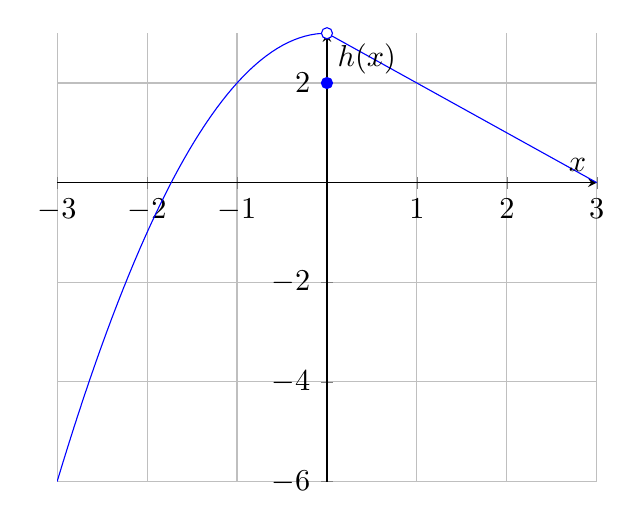
\begin{tikzpicture}
    \begin{axis}
        [grid, axis lines = center, xlabel = \(x\), ylabel=\(h(x)\)]
    \addplot[
    domain=-3:0,
    samples=50,
    color=blue,
    ]
    {-x^2+3};
    \addplot[mark=*,fill=white,draw=blue] coordinates{(0,3)};
    \addplot[mark=*,fill=blue,draw=blue] coordinates{(0,2)};
    \addplot[
    domain=0:3,
    samples=50,
    color=blue,
    ]
    {-x+3};
    \end{axis}
\end{tikzpicture}

From examining the graph, we see that $$\lim_{x\to0_-}h(x) = \lim_{x\to0_+}h(x) = 3$$
However, $h(0) = 2 \neq 3$. So, does this limit exist? It does! The limit of a function describes the \textit{behavior} of the function around a particular value, not the value of the function itself. In order for a limit to exist, the limits from the left and right must be equal to each other, but not necessarily the actual value of the function. 

\begin{Exercise}[title = Limits Practice 4, label=limits4]
Determine the limit from the left and the right for each function at the given value(s). State the limit at that value, if it exists.
    \begin{enumerate}
    \item $h(x), x=-1, 0, 1$
    \item $f(x), x=-1, 0, 2$
    \item $g(x), x=-2, 0, 1, 2$
\end{enumerate}
\end{Exercise}
\begin{Answer}[ref=limits4]
    \begin{enumerate}
    \item $\lim_{x\to-1_-}h(x) = 2$ and $\lim_{x\to-1_+}h(x)=2$, therefore the limit exists and $\lim_{x\to-1}h(x)=2$

    $\lim_{x\to0_-}h(x) = 3$ and $\lim_{x\to0_+}h(x)=3$, therefore the limit exists and $\lim_{x\to0}h(x)=3$

    $\lim_{x\to1_-}h(x) = 2$ and $\lim_{x\to1_+}h(x)=2$, therefore the limit exists and $\lim_{x\to1}h(x)=2$
    \item $\lim_{x\to-1_-}f(x)=2$ and $\lim_{x\to-1_+}f(x)=2$, therefore the limit exists and $\lim_{x\to-1}f(x) = 2$.

    $\lim_{x\to0_-}f(x) = 3$ and $\lim_{x\to0_+}f(x) = 0$, and because $\lim_{x\to0_-}f(x) \neq \lim_{x\to0_+}f(x)$, the limit does not exist.

    $\lim_{x\to2_-}f(x) = -2$ and $\lim_{x\to2_+}f(x) = -2$, therefore the limit exists and $\lim_{x\to2}f(x) = -2$.

    \item $\lim_{x\to-2_-}g(x) = -1$ and $\lim_{x\to-2_+}g(x) = -1$, therefore the limit exists and $\lim_{x\to-2}g(x) = -1$.

    $\lim_{x\to0_-}g(x)=1$ and $\lim_{x\to0_+}g(x) = 1$, therefore the limit exists and $\lim_{x\to0}g(x) = 1$

    $\lim_{x\to1_-}g(x) = 2$ and $\lim_{x\to0_+}g(x) = 1$, and because $\lim_{x\to1_-}g(x) = 2 \neq \lim_{x\to0_+}g(x)$, the limit does not exist.

    $\lim_{x\to2_-}g(x) = 0$ and $\lim_{x\to2_+}g(x) = 0$, therefore the limit exists and $\lim_{x\to2}g(x) = 0$
\end{enumerate}
\end{Answer}

A note about continuity:

In order to be able to talk more about limits and know when we can apply certain rules and theorems, we first must discuss continuity. A function is continuous if there are no "jumps" or "gaps" in the graph of the function. For example, the function $f(x) = x^2$ is continuous for all real values of x. On the other hand, the function $g(x) = tan(x)$ has many discontinuities, including at $x=\frac{\pi}{2}$. Let's examine the graph of each of these functions:

\begin{tikzpicture}
    \begin{axis}[
        grid,
        axis lines = center,
        xlabel = \(x\),
        ylabel = {\(f(x)\)},
        ]
    \addplot [
    domain=-3:3,
    samples=100,
    color=blue,
    ]
    {x^2};
    \end{axis}
\end{tikzpicture}

If you wanted, you could trace your finger along the graph of f(x) from $x=-3$ to $x=3$ without ever picking up your finger. This means the function is continuous in the domain from $-3 \leq x \leq 3$. In this case, the domain of continuity \textit{includes} the end points ($x=3$ and $x=-3$). This is called a closed interval. In other cases, the function will be continuous right up to, but not including, the endpoints, as with the domains of continuity for our other example, $g(x) = tanx$. This is called an open interval. Let's learn more about intervals of continuity by examining $g(x) = tanx$.

\begin{tikzpicture}
	\begin{axis}[
			axis lines=middle,
			axis line style={thick,<->},
			xmin=-2*pi-0.5,xmax=2*pi+0.5,ymin=-4.5,ymax=4.5,
			ytick={-4,-3,-2,-1,1,2,3,4},
			xtick={-2*pi,-1.5*pi,-pi,-0.5*pi,0,0.5*pi,pi,1.5*pi,2*pi},
			xticklabels={$-2\pi$,$-\frac{3}{2}\pi$,$-\pi$,$-\frac{1}{2}\pi$,$0$,$+\frac{1}{2}\pi$,$+\pi$,$+\frac{3}{2}\pi$,$+2\pi$},
			tick label style={font=\tiny},
			grid=major,
			major grid style={very thin,black},
			every axis plot post/.append style={thick},
			label style={font=\tiny},
			xlabel=$x$,
			ylabel=$g(x)$,
			smooth,
			%clip=false,restrict y to domain=-4:4,
			%legend style={
				%	font=\tiny,
					%legend cell align=left,
					%legend pos=outer north east,
					%draw=none,
					%empty legend},
			%legend entries={[blue]$y=\sin x$,[green]$y=\cos x$,[brown]$y=\tan x$}
			]
	%\addplot[domain=-2*pi:2*pi,samples=200,blue]{sin(deg(x))};
	%\addplot[domain=-2*pi:2*pi,samples=200,green]{cos(deg(x))};
	%\addplot[domain=-2*pi:2*pi,samples=200,brown]{tan(deg(x))};
	\addplot[domain=-2  *pi:-1.5*pi,samples=200,blue]{tan(deg(x))};
	\addplot[domain=-1.5*pi:-0.5*pi,samples=200,blue]{tan(deg(x))};
	\addplot[domain=-0.5*pi: 0.5*pi,samples=200,blue]{tan(deg(x))};
	\addplot[domain= 0.5*pi: 1.5*pi,samples=200,blue]{tan(deg(x))};
	\addplot[domain= 1.5*pi: 2  *pi,samples=200,blue]{tan(deg(x))};
        \draw[dashed, very thick, blue]  (axis cs: -3*pi/2,-5) -- (axis cs: -3*pi/2,5);
        \draw[dashed, very thick, blue]  (axis cs: -pi/2,-5) -- (axis cs: -pi/2,5);
        \draw[dashed, very thick, blue]  (axis cs: pi/2,-5) -- (axis cs: pi/2,5);
        \draw[dashed, very thick, blue]  (axis cs: 3*pi/2,-5) -- (axis cs: 3*pi/2,5);
	\end{axis}
\end{tikzpicture}

As you can see, if you trace your finger along the graph of the function starting at $x=0$, you can continue without lifting your finger to $x=\frac{\pi}{2}$. As you approach $x=\frac{\pi}{2}$ from the left, the value of $g(x)$ approaches $\infty$. In order to continue tracing the function PAST $x=\frac{\pi}{2}$, you have to lift your finger and bring it down to $-\infty$. The function then continues continuously again until $x=\frac{3\pi}{2}$. 

In the case of $g(x) = tan(x)$, the function is continuous on \textit{open intervals}, including the open interval $\frac{\pi}{2} < x < \frac{3\pi}{2}$.

There is a shorter way to represent open and closed domain intervals. We can represent that $f(x) = x^2$ is continuous on the closed interval $-3 \leq x \leq 3$ in the following way: $$x \in \left[3, -3 \right]$$

Which reads as "x contained in the domain -3 to 3, inclusive". That is, all the values from -3 to 3, including the endpoints. The inclusion of the endpoints is implied by the use of \textit{brackets}. For open intervals, we use parentheses to communicate that the interval goes up to, but does not include, the endpoints. For $g(x) = tanx$, we can use parentheses: $$x \in \left(\frac{-3\pi}{2}, \frac{-\pi}{2}\right)$$

because the $g(x) = tanx)$ is not continuous at $x=\frac{-3\pi}{2}$ or at $x=\frac{-\pi}{2}$.



Formally, a function $f(x)$ is continuous at $x=a$ if $\lim_{x\to a}f(x)$ exists \textit{and} $\lim_{x\to a}f(x) = f(a)$. That is, the limit is equal to the actual value of the function. Re-examine the graph of $h(x)$. We have already seen that $\lim_{x\to 0}h(x)$ exists and is equal to 3. However, $h(0) = 2 \neq \lim_{x\to0}h(x)$. So h(x) is not continuous at x = 0. Because $-x^2+3$ is evaluable all the way to $-\infty$ and $-x+3$ is evaluable all the way to $\infty$, the function h(x) is continuous everywhere \textit{except} $x=0$. We can represent this mathematically by saying $h(x)$ is continuous on the domain $x \in \left(-\infty, 0\right)\cup \left(0, \infty\right)$. We use parentheses for $\pm\infty$ because we can never actually reach $\infty$. Additionally, the function is continuous up to, but not including $0$, and the use of parentheses excludes $x=0$ from the domain of continuity.

\begin{Exercise}[title=Limits Practice 5, label=limits5]
State the location of discontinuities (if any) and explain why the fucntion is discontinuous at that location:
    \begin{enumerate}
    \item $f(x) = \frac{3x^2-8x-3}{x-3}$
    \item $f(x) = \begin{cases}
    \frac{2}{x^4}, \text{ if } x <\neq 0\\
    2, \text{ if } x=0
    \end{cases}$
    \item $f(x) = \begin{cases}
        \frac{3x^2-8x-3}{x-3}, \text{ if } x \neq 3\\
        1, \text{ if }, x=3
    \end{cases}$
\end{enumerate}
\end{Exercise}
\begin{Answer}[ref=limits5]
    \begin{enumerate}
    \item $f(x)$ is not defined at $x = 3$, therefore it is also discontinuous at $x = 3$. As we learn about the continuity of polynomials, we'll see why $f(x)$ is continuous everywhere else. 
    \item Here, $f(0)$ is defined, so we need to check if $\lim_{x \to 0}f(x) = f(0)$. The left and right limits as $x$ approaches $0$ are the same ($\infty$), so the limit exists. However, $f(0) = 1 \neq \lim_{x\to 0}f(x)$. Therefore, the function is discontinuous at $x=0$.
    \item In this function, $f(3)$ is defined, so we need to check if the limit equals the function value. The limit of $f(x)$ as $x$ approaches $3$ is: $$\lim_{x \to 3}\frac{3x^2-8x-3}{x-3} = \lim_{x \to 3}\frac{(3x+1)(x-3)}{x-3} = \lim_{x \to 3}3x+1 = 10$$ So the limit exists, but $$\lim{x \to 3}f(x) \neq f(3)$$ and we see that the function is discontinuous at $x=3$.
\end{enumerate}
\end{Answer}

There are some mathematical properties of limits which allow us to determine the limit of complex functions without seeing a graph or using a calculator to generate a table. 

The following laws are true given that \textit{c} is a constant, $\lim_{x\to a} f(x) $ exists, and $\lim_{x\to a} g(x) $ exists.

\begin{enumerate}
    \item Sum Law $\lim_{x\to a} \left[f(x) + g(x) \right] = lim_{x\to a} f(x) + lim_{x\to a} g(x)$
    \item Difference Law $\lim_{x\to a} \left[f(x) - g(x) \right] = lim_{x\to a} f(x) - \lim_{x\to a} g(x)$
    \item Constant Multiple Law $\lim_{x\to a} \left[\textit{c}f(x) \right] = \textit{c} \cdot \lim_{x\to a}    f(x) $
    \item Product Law $\lim_{x\to a} \left[f(x)g(x) \right] = lim_{x\to a}f(x) \cdot \lim_{x\to a} g(x)$
    \item Quotient Law $\lim_{x\to a} \frac{f(x)}{g(x)} = \frac{\lim_{x\to a} f(x)}{\lim_{x\to a} g(x)}$ given that $\lim_{x\to a} g(x) \neq 0$
\end{enumerate}
These laws are fairly obvious - the limit of the sum of two functions is equal to the sum of the limits of each function individually. The only tricky on is the last: the limit of the quotient of two functions is equal to the quotient of the limits if and only if the limit of the function in the denominator does not equal zero. This makes sense, since we know dividing by zero yields an undefined result. 

Let's practice applying these laws to evaluate the limits of the functions f(x), shown in blue below, and g(x), shown in red below:

$f(x) = \begin{cases}
    -x^2+3, \text{ if } x \leq 0\\
    -x, \text{ if } x > 0
\end{cases}$

$g(x) = \begin{cases}
   x^2+1, \text{ if } x < 1 \\
    (x-2)^2, \text{ if } x \geq 1
\end{cases}$

\begin{tikzpicture}
    \begin{axis}[
        grid,
        axis lines = center,
        xlabel = \(x\),
        ylabel = {\(y\)},
        ]
    \addplot [
    domain=-3:1,
    samples=50,
    color=red,
    ]
    {x^2+1};
    \addlegendentry{g(x)};
    \addplot[
    domain=-3:0,
    samples=50,
    color=blue,
    ]
    {-x^2+3};
    \addlegendentry{f(x)};
    \addplot[
    domain=1:3,
    samples=50,
    color=red,
    ]
    {(x-2)^2};
    \addplot[mark=*,fill=red,draw=red] coordinates{(1,1)};
    \addplot[mark=*,fill=white,draw=red] coordinates{(1,2)};
    
    \addplot[mark=*,fill=blue,draw=blue] coordinates{(0,3)};
    \addplot[mark=*, fill=white,draw=blue] coordinates{(0,0)};
    \addplot[
    domain=0:3,
    samples=50,
    color=blue,
    ]
    {-x};
    \end{axis}
\end{tikzpicture}

We can use these laws to evaluate limits involving $f(x)$ and $g(x)$ (shown on the graph above). Here are some examples:
Use the graphs of f(x) and g(x) given above to evaluate each limit, if it exists. If the limit does not exist, explain why. Two examples are given first:

Example 1: evaluate $\lim_{x\to0} f(x) \cdot g(x)$
From the Product Law, we know that:
$$\lim_{x\to0} f(x) \cdot g(x) = \lim_{x\to0}f(x) \cdot \lim_{x\to0} g(x)$$
Looking at the graph, we can see that $$\lim_{x\to0}g(x) = 1$$ and there is a discontinuity in $f(x)$ at $x=0$. Therefore, $$\lim_{x\to0}f(x) = \text{undef}$$. Substituting this, we get: $$\lim_{x\to0}f(x) \cdot \lim_{x\to0} g(x) = \text{undef} \cdot 1 = \text{undef}$$. Therefore, \textbf{the limit does not exist}. 

Example 2: evaluate $\lim_{x\to2}f(x) - g(x)$

Applying the Difference Law, we see that:

$$\lim_{x\to2}f(x) - g(x) = \lim_{x\to2}f(x) - \lim_{x\to2}g(x)$$

Examining the graph, we see that $$\lim_{x\to2}f(x) = -2$$ and $$\lim_{x\to2}g(x) = 0$$. Substituting these values, we get:

$$\lim_{x\to2}f(x) - g(x) = -2 - 0 = -2$$

\begin{Exercise}
    [title = Limits Practice 6, label=limits6]
\begin{enumerate}
    \item $\lim_{x\to-3} \frac{f(x)}{g(x)}$
    \item $\lim_{x\to2}\left[f(x) + 5g(x)\right]$
    \item $\lim_{x\to-1} \frac{3g(x)}{f(x)}$
    \item $\lim_{x\to0}f(x) \cdot 5g(x)$
    \item $\lim_{x\to-1} f(x) - 3g(x) $
\end{enumerate}
\end{Exercise}
\begin{Answer}
    [ref=limits6]
    \begin{enumerate}
        \item From the quotient law, we know that:$$\lim_{x\to3}\frac{f(x)}{g(x)}=\frac{\lim_{x\to3}f(x)}{\lim_{x\to3}g(x)}$$ From the graph, we see that: $$\lim_{x\to3}f(x) = -3$$ and that:$$\lim_{x\to3}g(x) = 1$$ Substituting these values, we get: $$\lim_{x\to3}\frac{f(x)}{g(x)}=\frac{-3}{1} = -3$$
        \item From the Sum Law, we know that: $$\lim_{x\to2}\left[f(x) + 5g(x)\right]=\lim_{x\to2}f(x) + \lim_{x\to2}5g(x)$$ and applying the Constant Multiple Law, we see that: $$\lim_{x\to2}\left[f(x) + 5g(x)\right]=\lim_{x\to2}f(x) + 5\lim_{x\to2}g(x)$$ Examining the graph of f(x) and g(x), we can determine that $$\lim_{x\to2}f(x) = -2$$ and $$\lim_{x/to2}g(x) = 0$$ Substituting these values, we get: $$\lim_{x\to2}\left[f(x) + 5g(x)\right]=-2 + 5 \cdot 0 = -2$$
        \item From the quotient law, we see that: $$\lim_{x\to-1} \frac{3g(x)}{f(x)}=\frac{\lim_{x\to-1}3g(x)}{\lim_{x\to-1}f(x)}$$ Applying the Constant Multiple Law, we get: $$\lim_{x\to-1} \left[\frac{3g(x)}{f(x)}\right]=\frac{3\lim_{x\to-1}g(x)}{\lim_{x\to-1}f(x)}$$ From the graph, we see that: $$\lim_{x\to-1}f(x) = 2$$ and $$\lim_{x\to-1}g(x) = 2$$ Substituting, we get: $$\lim_{x\to-1} \left[\frac{3g(x)}{f(x)}\right]=\frac{3 \cdot 2}{2}=3$$
        \item Applying the Product and Constant Multiple Laws, we get: $$\lim_{x\to0}\left[f(x) \cdot 5g(x)\right] = \lim_{x\to0}f(x) \cdot 5 \cdot \lim_{x\to0}g(x)$$ Examining the graphs, we see that $\lim_{x\to0}f(x)$ does not exist and $\lim_{x\to0}g(x) = 1$. Because $\lim_{x\to0}f(x)$ does not exist, $\lim_{x\to0}f(x) \cdot 5 \cdot \lim_{x\to0}g(x)$ also does not exist. 
        \item Applying the Difference and Constant Multiple Laws, we see that: $$\lim_{x\to-1} \left[f(x) - 3g(x)\right] =\lim_{x\to-1}f(x) - 3 \cdot \lim_{x\to-1}g(x)$$ Examining the graphs, we see that: $$\lim_{x\to-1}f(x) = 2$$ and $$\lim_{x\to-1}g(x) = 2$$ Substituting, we get that: $$\lim_{x\to-1} \left[f(x) - 3g(x)\right] =2 - 3 \cdot 2 = 2-6 = -4$$
    \end{enumerate}
\end{Answer}


Recall that exponents represent repeated multiplication. Therefore, if we apply the Product Law multiple times, we obtain the Power Law for limits:
\begin{enumerate}
    \setcounter{enumi}{5}
    \item Power Law $\lim_{x\to\infty} \left[f(x)\right]^n = \left[\lim_{x\to\infty}f(x)\right]^n$ where n is a positive integer
\end{enumerate}
There are two special limits that will be useful to us which are intuitively obvious, but we won't formally prove here.  
\begin{enumerate}
    \setcounter{enumi}{6}
    \item $\lim_{x\to a} \textit{c} = \textit{c}$
    \item $\lim_{x\to a} x = a$
\end{enumerate}
Combining Law 8 with the Power Law, we find that:
\begin{enumerate}
\setcounter{enumi}{8}
    \item $\lim_{x\to a} x^n = a^n$
\end{enumerate}
And similarly, for square roots:
\begin{enumerate}
    \setcounter{enumi}{9}
    \item $\lim_{x\to a} \sqrt[n]{x} = \sqrt[n]{a}$ (if n is even, we assume $a > 0$)
\end{enumerate}

Direct substitution property: If $f$ is a polynomial or rational function and $a$ is in the domain for $f$, then $$\lim_{x \to a}f(x) = f(a)$$

Often, rational functions can be simplified. In example BLANK FIXME, we computed the limit by simplifying $f(x) = \frac{3x^2-8x-3}{x-3}$ to the simpler $g(x) = 3x+1$. This is a valid strategy because $\frac{3x^2-8x-3}{x-3} = 3x+1$ when $x \neq 3$. Remember: a limit describes how a function behaves \textit{as it approaches} $a$, not its value/behavior when $x$ \textit{actually equals} $a$. This reveals the following useful rule: $$\text{If } f(x)=g(x) \text{ when } x \neq a \text{, then } \lim_{x \to a}f(x) = \lim_{x \to a}g(x) \text{, provided the limit exists.}$$

%Here is a function:
%
%$$f(x) = \frac{x^2}{x} + 1$$
%
%This $f$ is defined for any real number \emph{except 0}. (You can't
%divide anything, including zero, by zero.)
%
%Let's plot $f$:
%
%\begin{tikzpicture}[
%tl/.style = {% tick labels
%    fill=white, inner sep=1pt, font=\scriptsize,
%            },                        ]
%% grid
%\draw[sdkblue, very thin] (-3,-3) grid (3,3);
%
%
%    \draw[<->,thick,dashed] (-3.2,0) -- (3.2,0) node[right] {$x$};
%    \draw[<->,thick,dashed] (0,-3.2) -- (0, 3.2) node[above] {$y$};
%% curve
%\draw[<-,draw=black,thick,domain=-3:-0.1,samples=300,variable=\x] plot (\x,{\x + 1});
%\draw[thick] (0,1) circle (0.1);
%\draw[->,draw=black,thick,domain=0.1:2,samples=300,variable=\x] plot (\x,{\x + 1});
%\end{tikzpicture}
%
%You can see that the function is the same as $x + 1$ everywhere except
%$x = 0$.  You can see that as the function approaches $x=0$ from the
%left, the value of the function approaches 1.  You can see that as the
%function approaches $x=1$ from the right, the value of the function
%approaches 1.
%
%Mathematicians say ``The \newterm{limit} of $f$ as $x$ approaches 0, is 1.''  We have a notation for this:
%
%$$\lim_{x \rightarrow 0} f(x) = 1$$
%
%We generally use limit whenever we mean ``We are getting arbitrarily
%close, but we can never really get there.''  For example, you might
%say ``The limit of $1/t$ as $t$ goes to infinity is 0.''
%
%\begin{tikzpicture}[
%tl/.style = {% tick labels
%    fill=white, inner sep=1pt, font=\scriptsize,
%            },                        ]
%% grid
%\draw[sdkblue, very thin] (-5,-5) grid (5,5);
%    \draw[<->,thick,dashed] (-5.2,0) -- (5.2,0) node[below] {$t$};
%    \draw[<->,thick,dashed] (0,-5.2) -- (0, 5.2);
%% curve
%\draw[<->,draw=black,thick,domain=0.2:5,samples=300,variable=\x] plot (\x,{1/\x});
%\draw[<->,draw=black,thick,domain=-5:-0.2,samples=300,variable=\x] plot (\x,{1/\x});
%\draw (5.0, 0.2) node[above] {$t \rightarrow \infty$, $1/t \rightarrow 0$};
%\draw (0.0, 5.2) node[above] {$t \rightarrow 0$ from the right, $1/t \rightarrow \infty$};
%\draw (0.0, -5.2) node[below] {$t \rightarrow 0$ from the left, $1/t \rightarrow -\infty$};
%\draw (-5.0, -0.2) node[below] {$t \rightarrow -\infty$, $1/t \rightarrow 0$};
%
%\end{tikzpicture}
%
%What is the limit of $1/t$ as $t$ approaches zero? The limit isn't
%defined because if you approach from the right, $1/t$ goes to
%infinity, but if you approach from the left, $1/t$ goes to negative
%infinity.

\graphicspath{{../../Chapters/differentiation/en_US}}
\chapter{Differentiation}

We have done some differentiation, but you haven't been given the real
definition because it is based on limits.

The idea is that we can find the slope between two points on the graph
$a$ and $b$ like this:

$$m = \frac{f(b) - f(a)}{b - a}$$

\begin{tikzpicture} [scale=2]
\draw[->,thick,sdkblue] (0,0) -- (4,0) node[right] {$x$};
\draw[->,thick,sdkblue] (0,0) -- (0, 3.45) node[above] {$y$};
% curve
\draw[<->,thick,draw=black, domain=0:3.7,samples=300,variable=\x]  plot (\x,{\x * \x * 0.25});
\draw [sdkblue] (1, 0.25) -- (3, 2.251);
\draw [dashed] (1,0.25) -- (1, 0) node[below]{$a$};
\draw [dashed] (3, 2.251) -- (3, 0) node[below]{$b$};
\draw [dashed] (1,0.25) -- (3, 0.25) node[right] {$f(a)$};
\draw (3,2.251) node[right] {$f(b)$};
\draw (1,0.25) circle (0.05);
\draw (3, 2.251) circle (0.05);
\draw (2, 0.25) node[above]{$b - a$};
\draw (3, 1.25) node[right] {$f(b) - f(a)$};
\end{tikzpicture}

If we want to find the slope at $a$ we take the limit of this as the $b$ goes to $a$:

$$f'(a) = \lim_{b \rightarrow b}\frac{f(b) - f(a)}{b - a}$$

This idea is usually expressed using $\Delta x$ as the difference between $b$ and $a$:

\begin{tikzpicture} [scale=2]
\draw[->,thick,sdkblue] (0,0) -- (4,0) node[right] {$x$};
\draw[->,thick,sdkblue] (0,0) -- (0, 3.45) node[above] {$y$};
% curve
\draw[<->,thick,draw=black, domain=0:3.7,samples=300,variable=\x]  plot (\x,{\x * \x * 0.25});
\draw [sdkblue] (1, 0.25) -- (3, 2.251);
\draw [dashed] (1,0.25) -- (1, 0) node[below]{$a$};
\draw [dashed] (3, 2.251) -- (3, 0) node[below]{$a + \Delta x$};
\draw [dashed] (1,0.25) -- (3, 0.25) node[right] {$f(a)$};
\draw (3,2.251) node[right] {$f(a + \Delta x)$};
\draw (1,0.25) circle (0.05);
\draw (3, 2.251) circle (0.05);
\draw (2, 0.25) node[above]{$\Delta x$};
\draw (3, 1.25) node[right] {$f(a + \Delta x) - f(a)$};
\end{tikzpicture}

Then the formula becomes:

$$f'(a) = \lim_{\Delta x \rightarrow 0}\frac{f(a + \Delta x) - f(a)}{\Delta x}$$

Now, at any point $a$ we can compute the slope of the line tangent to the function at $a$:

\begin{tikzpicture} [scale=2]
\draw[->,thick,sdkblue] (0,0) -- (4,0) node[right] {$x$};
\draw[->,thick,sdkblue] (0,0) -- (0, 3.45) node[above] {$y$};
% curve
\draw[<->,thick,draw=black, domain=0:3.7,samples=300,variable=\x]  plot (\x,{\x * \x * 0.25});
\draw [sdkblue] (0, -0.25) -- (3, 1.25) node[midway, right]{slope = $f'(a)$};;
\draw [dashed] (1,0.25) -- (1, 0) node[below]{$a$};
\draw (1,0.25) circle (0.05);
\end{tikzpicture}

\section{Differentiability}

Warning: Not every function is differentiable everywhere.  For
example, if $f(x) = |x|$, you get a corner at zero.

\begin{tikzpicture} [scale=1]
\draw[->,thick,sdkblue] (-4,0) -- (4,0) node[right] {$x$};
\draw[->,thick,sdkblue] (0,0) -- (0, 3.45) node[above] {$y$};
% curve
\draw[->,thick,draw=black, domain=0:3.7,samples=300,variable=\x]  plot (\x,\x);
\draw[<-,thick,draw=black, domain=-3.7:0,samples=300,variable=\x]  plot (\x,{-1 * \x});
\end{tikzpicture}

To the left of zero, the slope is -1. To the right of zero, the slope
is 1.  At zero?  The derivative is not defined.

If a function has a derivative everywhere, it is said to be
\newterm{differentiable}. Generally, you can think of differentiable
functions as smooth -- their graphs have no corners.

\section{Using the definition of derivative}

Let's say that you want to know the slope of $f(x) = -3x^2$ at $x = 2$.
Using the definition of the derivative, that would be:

$$f'(2) = \lim_{\Delta x \rightarrow 0}\frac{f(2 + \Delta x) - f(2)}{\Delta x} = \lim_{\Delta x \rightarrow 0}\frac{-3(2 + \Delta x)^2- \left(-3(2)^2\right)}{\Delta x} = \lim_{\Delta x \rightarrow 0}\frac{-12 - 12\Delta x + -3(\Delta x)^2 + 12}{\Delta x} = -12$$ 



\graphicspath{{../../Chapters/discrete_probability/en_US}}
\chapter{Introduction to Discrete Probability}

First, let's take care of the word \emph{discrete} vs \emph{discreet}.
They sound exactly the same, but ``discrete'' means ``individually
separate and distinct'' and ``discreet'' means ``careful about what
other people know''.  So you might say, ``You can think of light as a
continuous wave or as a blast of discrete particles.'' And you might
say, ``Please go get the box of doughnuts from the kitchen. Oh, and
there are a lot of hungry people in the house, so be
discreet.''\index{discrete vs. discreet}

When we are talking about probabilities, some problems deal
with discrete quantities like ``What is the probability that I will
throw these three dice and the numbers that roll face up sum to 9?''. There
are also problems that deal with continuous properties like ``What is
the probability that the next bird to fly over my house will weigh
between 97.2 and 98.1 grams ?'' In this module, we are going to focus
on the probability problems that deal with discrete quantities.

Watch Khan Academy's Introduction to Probability at \url{https://youtu.be/uzkc-qNVoOk}.

Let's say that I have a cloth sack filled with 100 marbles; 99 are red
and 1 is white. If I ask you to reach in without looking and pull out
one marble, you will probably pull out a red one. We say that ``There
is a 1 in 100 chance that you would pull out a white marble.'' Or we
can use percentages and say ``There is a 1\% chance that you will pull
out a white marble.'' Or we can use decimals and say ``There is a 0.01
probability that you will pull out a white marble.''
% Bag Diagram
In probability, we often talk about the probability of certain
events. ``Pulling out a white marble'' is an event, and we can give it
a symbol like $W$. Then, in equations we use $p$ to mean ``the
probability of''.  Thus, we can say ``There is a 0.01 probability that
you will pull out a white marble'' which becomes the equation
\begin{equation*}
  p(W) = 0.01
\end{equation*}\index{probability}
% ADD: Make sure functions come before this chapter, connect to functions

\section{The Probability of All Possibilities is 1.0}

We know that you are either going to pull out a red marble or a white marble,
so the probability of a white marble being pulled and the probability
of a red marble being pulled must add up to 100\%. Therefore, the odds of
pulling out a red marble must be 99\% or 0.99. If we let the event ``Pull out a red marble'' be given by the symbol $R$, we can say:
\begin{equation*}
  p(R) = 1.0 - P(W) = 1.0 - 0.01 = 0.99
\end{equation*}

Now, let's say that I make you take a marble from the bag and then
toss a coin. What is the probability that you will pull a white marble
and then get heads on the coin? It is the product of the two
probabilities: $0.01 \times 0.5 = 0.005$, so one-half of a one percent
chance. Do the probabilities still sum to 1?
\begin{itemize}
\item White and Heads = $0.01 \times 0.5 = 0.005$
\item White and Tails = $0.01 \times 0.5 = 0.005$
\item Red and Heads = $0.99 \times 0.5 = 0.495$
\item Red and Tails = $0.99 \times 0.5 = 0.495$
% ADD: add up the values at the end for clarity
\end{itemize}
Yes, the probabilitites of all the possibilities still add to 1.

\section{Independence}

In the last section, I told you that the probability of two events
(``Pulling a red marble from the bag'' and ``Getting tails in a coin
toss'') is the product of the probability of each event: $0.99 \times 0.5 = 0.495$.

This is true if the two events are \textit{independent}, that is the
outcome of one doesn't change the probability of the other.  The
example I gave is independent: It doesn't matter what ball you pull
from the bag, the outcome of the coin toss will always be 50-50.\index{independent}

What are two events that are not independent? The probability that a
person is a professional basketball player and the probability that
someone wears a shoe that is size 13 or larger is \textit{not}
independent. After all, height is an advantage in basketball and most
tall people also have large feet. So if you know someone is a
basketball player, they likely wear large shoes.
% ADD: Correlation for Causeation 
% Weird Correlations Website: https://www.tylervigen.com/spurious-correlations
% KA: https://youtu.be/R-NeYKSEqns

\begin{Exercise}[title={Rolling Dice}, label=rolling-dice]
  If I give you three dice to roll, what is the
  probability that you will roll a 5 on all three dice?
\end{Exercise}
\begin{Answer}[ref=rolling-dice]
  probability of all 5's $ = \frac{1}{6}\times\frac{1}{6}\times\frac{1}{6} = \left(\frac{1}{6}\right)^3 = \frac{1}{216} \approx 0.0046$
  \end{Answer}
    
\begin{Exercise}[title={Flipping Coins}, label=flipping-coins]
  If I give you five coins to flip, what is the
  probability that at least one coin will come up heads?
\end{Exercise}
\begin{Answer}[ref=rolling-dice]
  probability of at least one heads = 1.0 - probability of all tails $ = 1.0 - \left(\frac{1}{2}\right)^5 =1.0 - \frac{1}{32} = \frac{31}{32} = \approx 0.97$ 
  \includegraphics[width=0.5\textwidth]{coin_prob.png}
\end{Answer}
    
\section{Why 7 is the most likely sum of two dice}

If you roll two dice, the sum will be 2 or 12 or any number in
between. It is very tempting to assume that the likelihood of any of
those numbers is the same. In fact, the probability of a 2 is
$\frac{1}{36} \approx 3\%$ and the probability of a 7 is $\frac{1}{6}
\approx 17\%$. A 7 is six times more likely than a 12! Why?

When you roll the first die, there are six possibilities with equal
probability. When you roll the second die, there are six possibilities
with equal probability. so there are a total of 36 possible events
with equal probabilities: 1 then 1, 1 then 2, 2 then 1, 1 then 3, 3
then 1, etc. Only one of these (1 then 1) adds to 2.  But six of these
sum to 7: 1 then 6, 6 then 1, 2 then 5, 5 then 2, 3 then 4, 4 then
3. So a 7 is six times more likely than a 2.

Here is the complete table:
%Dice Diagram
\begin{tabular}{c| c c c c c c | c | c}
  Sum &     &     &     &     &     &     & Count & Probability \\
  \hline
  2   & 1,1 &     &     &     &     &     &   1    & 1/36 \\
  3   & 1,2 & 2,1 &     &     &     &     &   2    & 1/18 \\
  4   & 1,3 & 2,2 & 3,1 &     &     &     &   3    & 1/12 \\
  5   & 1,4 & 2,3 & 3,2 & 4,1 &     &     &   4    & 1/9 \\
  6   & 1,5 & 2,4 & 3,3 & 4,2 & 5,1 &     &   5    & 5/36 \\
  7   & 1,6 & 2,5 & 3,4 & 4,3 & 5,2 & 6,1 &   6    & 1/6 \\
  8   &     & 2,6 & 3,5 & 4,4 & 5,3 & 6,2 &   5    & 5/36 \\
  9   &     &     & 3,6 & 4,5 & 5,4 & 6,3 &   4    & 1/9 \\
  10  &     &     &     & 4,6 & 5,5 & 6,4 &   3    & 1/22 \\
  11  &     &     &     &     & 5,6 & 6,5 &   2    & 1/18 \\
  12  &     &     &     &     &     & 6,6 &   1    & 1/36
\end{tabular}

When I bumped into this, I was skeptical. I decided to test it, so I
rolled a pair of dice hundreds of times and made a histogram. It was a
tedious and time-consuming task -- just the sort of thing that we make
computers do for us.
% ADD: Define Histogram
\includegraphics[width=0.5\textwidth]{dice_histogram.png}
\section{Random Numbers and Python}

You are going to write a simulation of rolling dice in Python. To do
this, you will need to generate a random sequence of numbers. The
numbers will need to be in the range 1 to 6, and they will need to
appear in the sequence with the same frequency.  We say the sequence
will follow \textit{the uniform distribution}.  That is, the
probability is uniformly distributed among the 6 possibilities.\index{random number generation}

Start python and try a few of the different ways to generate random numbers:
\begin{Verbatim}[commandchars=\\\{\}]
> \textbf{python3}
>>> \textbf{import random}
>>> \textbf{random.random()}  # Generates a random floating point number between 0 and 1
0.6840892758539989
>>> \textbf{randrange(5)}      # Generates an integer in the range 0 - 4
2
>>> \textbf{x = ['Rock', 'Paper', 'Scissors']}
>>> \textbf{random.choice(x)}   # Pick a random entry from the sequence
'Paper'
>>> \textbf{x}
['Rock', 'Paper', 'Scissors'] 
>>> \textbf{random.shuffle(x)}   # Shuffle the order of the sequence
>>> \textbf{x}
['Scissors', 'Paper', 'Rock']
>>> \textbf{a = list(range(30))}
>>> \textbf{a}
[0, 1, 2, 3, 4, 5, 6, 7, 8, 9, 10, 11, 12, 13, 14, 15,
  16, 17, 18, 19, 20, 21, 22, 23, 24, 25, 26, 27, 28, 29, 29]
>>> \textbf{random.sample(a, 10)} # Return 10 randomly chosen items from the sequence
[8, 7, 20, 9, 25, 13, 23, 11, 14, 16]
\end{Verbatim}
% KA: https://www.youtube.com/watch?v=Jua-KWBdzfU
Clearly, Python has a lot of ways to do things that look random. I
should be honest with you at this point: they aren't really
random. The computer that you are using can't generate random
data. Instead, it uses tricks to create data that looks random; we
call this \textit{pseudorandom} data. Good pseudorandom algorithms are
very important for cryptography and data security.

What if you want real random data? Some companies that are using
the decay of radioactive materials to generate real random data. You
can pay to download it. For our purposes, Python's pseudorandom
numbers are quite sufficient.

If we generate two random numbers in the range 1 through 6 and add them together, we
will have simulated rolling a pair of dice. Like this:

\begin{Verbatim}[commandchars=\\\{\}]
>>> \textbf{a = random.randrange(6) + 1}
>>> \textbf{b = random.randrange(6) + 1}
>>> \textbf{a + b}
8
\end{Verbatim}

First, let's write a program that just rolls the dice 100 times and shows the result. Make a file \url{dice.py}:
\begin{Verbatim}
import random

roll_count = 100

for i in range(roll_count):
    a = random.randrange(6) + 1
    b = random.randrange(6) + 1
    roll = a + b
    print(f"Toss {i}: {a} + {b} = {roll}")
\end{Verbatim}

When you run it, you should see something like:
\begin{Verbatim}[commandchars=\\\{\}]
> \textbf{python3 dice.py}
Toss 0: 6 + 6 = 12
Toss 1: 4 + 4 = 8
Toss 2: 4 + 2 = 6
Toss 3: 4 + 6 = 10
Toss 4: 4 + 4 = 8
...
Toss 98: 5 + 2 = 7
Toss 99: 5 + 2 = 7
\end{Verbatim}

Now we want to count occurrences of each possible outcome. Let's use an
array of integers. We will start with an array of zeros. And, for
example, when we roll a 3, we'll add 1 to item 3 in the array. (We can
never roll a zero or a one, so those two entries will always be zero.)
% ADD: Define Array
\begin{Verbatim}[commandchars=\\\{\}]
import random

roll_count = 100

\textbf{# Make an array containing 13 zeros}
\textbf{counts = [0] * 13}

for i in range(roll_count):
    a = random.randrange(6) + 1
    b = random.randrange(6) + 1
    roll = a + b
    print(f"Toss {i}: {a} + {b} = {roll}")

    \textbf{# Increment the count for roll}
    \textbf{counts[roll] += 1}

\textbf{print(f"Counts: {counts}")}
\end{Verbatim}

When you run this, at the end you will see a count for each possible outcome :

\begin{Verbatim}
...
Toss 98: 3 + 2 = 5
Toss 99: 6 + 1 = 7
Counts: [0, 0, 2, 6, 16, 11, 13, 14, 11, 11, 6, 9, 1]
\end{Verbatim}

What was the count that we expected? For example, we expected to see a
2 about once every 36 rolls, right? It might be nice to compare our
count to what we expected. Add a few more lines, and we are going to
increase the number of rolls. You will probably want to delete the
line that prints each roll separately:

\begin{Verbatim}[commandchars=\\\{\}]
import random

\textbf{# Can't ever be 0 or 1}
\textbf{p = [0.0, 0.0, 1/36, 1/18, 1/12, 1/9, 5/36, 1/6, 5/36, 1/9, 1/12, 1/18, 1/36]}
roll_count = 1000

# Make an array containing 13 zeros
counts = [0] * 13

for i in range(roll_count):
    a = random.randrange(6) + 1
    b = random.randrange(6) + 1
    roll = a + b

    # Increment the count for roll
    counts[roll] += 1

\textbf{for i in range(2,13):}
    \textbf{print(f"{i} appeared {counts[i]} times, expected {p[i] * roll_count:.1f}")}
\end{Verbatim}

Now you should see something like:
\begin{Verbatim}
2 appeared 39 times, expected 27.8
3 appeared 55 times, expected 55.6
4 appeared 84 times, expected 83.3
5 appeared 110 times, expected 111.1
6 appeared 160 times, expected 138.9
7 appeared 176 times, expected 166.7
8 appeared 124 times, expected 138.9
9 appeared 93 times, expected 111.1
10 appeared 87 times, expected 83.3
11 appeared 49 times, expected 55.6
12 appeared 23 times, expected 27.8
\end{Verbatim}

Whenever you are dealing with random numbers, the outcome will seldom
be \textit{exactly} what you expected. In this case, however, you should see that your
predictions are pretty close.

\subsection{Making a bar graph}



A bar graph is a nice way to look at quantities like this.  Let's make a bar graph that shows the actual count and the expected count:\index{bar graph!in python}

\includegraphics[width= 0.85\textwidth]{dice1.png}

We need to describe the set of rectangles, to do this we will loop through each possible roll (2 - 12) and put data in four lists for each:
% ADD: Define lists
\begin{Verbatim}[commandchars=\\\{\}]
import random
\textbf{import matplotlib.pyplot as plt}

# Can't ever be 0 or 1
p = [0.0, 0.0, 1/36, 1/18, 1/12, 1/9, 5/36, 1/6, 5/36, 1/9, 1/12, 1/18, 1/36]
roll_count = 1000

# Make an array containing 13 zeros
counts = [0] * 13

for i in range(roll_count):
    a = random.randrange(6) + 1
    b = random.randrange(6) + 1
    roll = a + b

    # Increment the count for roll
    counts[roll] += 1

\textbf{# Gather data for bar chart}
\textbf{bar_width = 0.35}
\textbf{expected = []}
\textbf{actual_starts = []}
\textbf{expected_starts = []}
\textbf{labels = []}
\textbf{actual = []}
for i in range(2,13):
    \textbf{expected.append(p[i] * roll_count)}
    \textbf{actual.append(counts[i])}      
    \textbf{actual_starts.append(i - bar_width/2)}
    \textbf{expected_starts.append(i + bar_width/2)}
    \textbf{labels.append(i)}
    
\textbf{fig, ax = plt.subplots()}
    
\textbf{# Create the bars}
\textbf{ax.bar(actual_starts, actual, bar_width, label='Actual')}
\textbf{ax.bar(expected_starts, expected, bar_width, label='Expected')}
\textbf{ax.set_xticks(labels)}

\textbf{# Provide labels}
\textbf{ax.set_ylabel('Occurences')}
\textbf{ax.set_title('Dice Rolls')}
\textbf{ax.legend()}
\textbf{plt.show()}
\end{Verbatim}

% ADD: For extra guideance: https://pythoniseasytolearn.blogspot.com/2019/09/rolling-two-dice.html
\graphicspath{{../../Chapters/combinatorics/en_US}}
\chapter{Beginning Combinatorics}

Discrete probability problems often include some counting. For
example, we figured out that there were 36 different ways the two dice, 
but all of them summed to some number 2 through 12. How
many different ways could three 8-sided dice come up? We would need to
count them, right? As the numbers get big we will need some tricks so
we don't need to write them all down and count them one-by-one.

The branch of mathematics that focuses on tricks for counting is
called \textit{combinatorics}.\index{combinatorics}
% KA: https://www.khanacademy.org/computing/pixar/crowds/crowds-1/v/combinatorics1

How can we be sure that there were 36 different configurations for the
two 6-sided dice? The first die could have come up as any one of six
numbers. For each of those, the second could have come up with any one
of six numbers. Thus, the number of possibilities is $ 6 \times 6 =
36.$

How many different configurations for 3 8-sided dice?  $8 \times 8
\times 8 = 8^3 = 512$.

What about seven dice, each with 20 sides? There would be $20^7=1,280,000,000$
configurations. See, aren't you glad we don't need to write them all
down?

Now, let's say that six people (Anne, Brock, Carl, Dev, Edgar, and Fred) are
going to run a race. You have to make a plaque that says who won first
place, who won second place, and who won third. If you want to get all
the possible plaques created beforehand, and just pull the right one
out as soon as the race ends, how many plaques would you need to get
engraved?

% \includegraphics[width=0.8\textwidth]{Race.png}

In this case, once someone has been given first place, they can't win
second or third place. Thus, any of the 6 people can come in first,
but once you have engraved that person's name on the plaque, there are
only 5 people whose names can appear in second place. Once you have
engraved that name, there are only 4 people whose names can appear in
third place. Thus, you would get $6 \times 5 \times 4 = 120$ plaques
engraved.
% ADD: This situation is a little confusing given if they're doing the plaques before hand, they wouldn't know who came in each place

What if the plaque includes all 6 places?  Then you would need $6 \times 5
\times 4 \times 3 \times 2 \times 1 = 720$ plaques engraved.  We use
this process often enough that we gave it a name.  We say ``I need 6
factorial plaques engraved.''  When we write a factorial, we use an
exclamation point:\index{factorial}
% ADD: Same issue here

$$6! = 6 \times 5 \times 4 \times 3 \times 2 \times 1 = 720$$

We use the word ``permutation'' to mean a particular ordering.
This rule says $n$ items can be ordered in $n!$ ways. Thus
mathematicians actually say ``If you have a list of $n$ items then we
can generate $n!$ different permutations of those items''.

In Python, there is a \pyfunction{factorial} function in the math library:
\begin{Verbatim}[commandchars=\\\{\}]
> \textbf{python3} 
>>> \textbf{import math}
>>> \textbf{math.factorial(6)}
720
\end{Verbatim}

Handy, right? Now you don't need to write a loop to calculate factorials.

Remember when we only wanted the first three names on the plaque? We can do that problem using factorials:

$$6 \times 5 \times 4 = \frac{6 \times 5 \times 4 \times 3 \times 2 \times 1}{3 \times 2 \times 1} = \frac{6!}{3!}$$

This formulation makes it easy to figure out on any calculator with a ``!'' button.

The rule on this is to fill $m$ positions from $n$ items, it can be done this many ways:

$$\frac{n!}{(n-m)!}$$
% KA: https://www.khanacademy.org/computing/pixar/crowds/crowds2/v/combinatorics8

\subsection{Choose}

Let's say that there are 12 kids in a classroom, and you need a team
of 4 to wipe down the desks. How many different possible teams are
there? You know that if you were giving out four different positions
(Like the race gave out 1st, 2nd, and 3rd), the answer would be $12
\times 11 \times 10 \time 9$ or $12! / (12 - 4)!$.
% ADD: This is the probability that one person would be chosen

However, once we pick the 4 people, we don't care what order they are
in, right?  In this problem, the team ``Anne, Brad, Carl, and Don'' is
the same as the team ``Carl, Don, Brad, and Anne''.

Thus, the quantity $12! / (12 - 4)!$ is many times too large because
it counts each permutation separately. To get the right number, we
just divide this by the number of possible permuations for a group of
four people: $4!$

That gets us our answer: How many different teams of four can be chosen from 12 people?

$$\frac{12!}{(12-4)! 4!}= 495$$
% ADD: Needs a bit more explanation for claretiy, might just be my understanding
In combinatorics, we use this quantity a lot, so we have given it a name: \textit{choose}\index{choose function}

We have also given it a notation. ``12 choose 4'' is written like this:

$${12 \choose 4}$$
% KA Binomial Therom: https://www.khanacademy.org/math/precalculus/x9e81a4f98389efdf:series/x9e81a4f98389efdf:binomial/v/binomial-theorem

Python has the \pyfunction{math.comb} function:

\begin{Verbatim}[commandchars=\\\{\}]
> \textbf{python3}
>>> \textbf{import math}
>>> \textbf{comb(12, 4)}
495  
\end{Verbatim}


\graphicspath{{../../Chapters/permutations/en_US}}
\chapter{Introduction to the Kontinua Sequence}

This book will start you on the long and difficult trek to becoming a modern
problem solver. Along the path, you will learn how to use the tools of
math, computers, and science.

Why should you bother? There are big problems in this world that will
require expert problem solvers. Those people will make the world a
better place while enjoying interesting and lucrative careers. We are
talking about engineers, scientists, doctors, computer programmers,
architects, actuaries, and mathematicians. Right now, those occupations represent
about 6\% of all the jobs in the United States. Soon,
that number is expected to rise above 10\%.  On average, people in
that 10\% of the population are expected to have salaries twice that
of their non-technical counterparts.\index{career}

Solving problems is difficult. At some point on this journey, you will
see people who are better at solving problems than you are. You, like
every other person who has gone on this journey, will think ``I have
worked so hard on this, but that person is better at it than
I am. I should quit.'' Don't.\index{quitting}

First, solving problems is like a muscle. The more you do, the better
you get at it.  It is OK to say ``I am not good at this yet.'' That
just means you need more practice.

Second, you don't need to be the best in the world. 10 million people
your age can be better at solving problems than you, \textit{and you
  can still be in the top 10\% of the world}. If you complete this
journey, there will be problems for you to solve and a job where your
problem-solving skills will be appreciated.

\emph{Where do we start?}

The famous physicist Richard Feynman once asked this question: ``If,
in some cataclysm, all of scientific knowledge were to be destroyed,
and only one sentence was passed on to the next generation of
creatures, what statement would contain the most information in the
fewest words?''

His answer was ``All things are made of atoms—little particles that move around in
perpetual motion, attracting each other when they are a little
distance apart, but repelling upon being squeezed into one another.''

\emph{That} seems like a good place to start.

\graphicspath{{../../Chapters/conditional_prob/en_US}}
\chapter{Introduction to the Kontinua Sequence}

This book will start you on the long and difficult trek to becoming a modern
problem solver. Along the path, you will learn how to use the tools of
math, computers, and science.

Why should you bother? There are big problems in this world that will
require expert problem solvers. Those people will make the world a
better place while enjoying interesting and lucrative careers. We are
talking about engineers, scientists, doctors, computer programmers,
architects, actuaries, and mathematicians. Right now, those occupations represent
about 6\% of all the jobs in the United States. Soon,
that number is expected to rise above 10\%.  On average, people in
that 10\% of the population are expected to have salaries twice that
of their non-technical counterparts.\index{career}

Solving problems is difficult. At some point on this journey, you will
see people who are better at solving problems than you are. You, like
every other person who has gone on this journey, will think ``I have
worked so hard on this, but that person is better at it than
I am. I should quit.'' Don't.\index{quitting}

First, solving problems is like a muscle. The more you do, the better
you get at it.  It is OK to say ``I am not good at this yet.'' That
just means you need more practice.

Second, you don't need to be the best in the world. 10 million people
your age can be better at solving problems than you, \textit{and you
  can still be in the top 10\% of the world}. If you complete this
journey, there will be problems for you to solve and a job where your
problem-solving skills will be appreciated.

\emph{Where do we start?}

The famous physicist Richard Feynman once asked this question: ``If,
in some cataclysm, all of scientific knowledge were to be destroyed,
and only one sentence was passed on to the next generation of
creatures, what statement would contain the most information in the
fewest words?''

His answer was ``All things are made of atoms—little particles that move around in
perpetual motion, attracting each other when they are a little
distance apart, but repelling upon being squeezed into one another.''

\emph{That} seems like a good place to start.

\graphicspath{{../../Chapters/bayes/en_US}}
\chapter{Introduction to the Kontinua Sequence}

This book will start you on the long and difficult trek to becoming a modern
problem solver. Along the path, you will learn how to use the tools of
math, computers, and science.

Why should you bother? There are big problems in this world that will
require expert problem solvers. Those people will make the world a
better place while enjoying interesting and lucrative careers. We are
talking about engineers, scientists, doctors, computer programmers,
architects, actuaries, and mathematicians. Right now, those occupations represent
about 6\% of all the jobs in the United States. Soon,
that number is expected to rise above 10\%.  On average, people in
that 10\% of the population are expected to have salaries twice that
of their non-technical counterparts.\index{career}

Solving problems is difficult. At some point on this journey, you will
see people who are better at solving problems than you are. You, like
every other person who has gone on this journey, will think ``I have
worked so hard on this, but that person is better at it than
I am. I should quit.'' Don't.\index{quitting}

First, solving problems is like a muscle. The more you do, the better
you get at it.  It is OK to say ``I am not good at this yet.'' That
just means you need more practice.

Second, you don't need to be the best in the world. 10 million people
your age can be better at solving problems than you, \textit{and you
  can still be in the top 10\% of the world}. If you complete this
journey, there will be problems for you to solve and a job where your
problem-solving skills will be appreciated.

\emph{Where do we start?}

The famous physicist Richard Feynman once asked this question: ``If,
in some cataclysm, all of scientific knowledge were to be destroyed,
and only one sentence was passed on to the next generation of
creatures, what statement would contain the most information in the
fewest words?''

His answer was ``All things are made of atoms—little particles that move around in
perpetual motion, attracting each other when they are a little
distance apart, but repelling upon being squeezed into one another.''

\emph{That} seems like a good place to start.

%%%%%%%%%%%%%%%%%%%%%%%%%%%%%%%%%
%% Bookfooter.tex by Aaron Hillegass
%% Nov 8, 2020

\appendix

\chapter{Answers to Exercises}
\shipoutAnswer

\bibliography{references}

\printindex

\end{document}